%!TEX program = lualatex

\documentclass{beamer}
%\documentclass[aspectratio=169]{beamer}

\usepackage{fontspec}
\usepackage{libertine}
\usepackage{microtype}
\usepackage{amssymb}
\usepackage{mathtools}
\usepackage{unicode-math}
\usepackage{lualatex-math}

\setmainfont[Ligatures=TeX]{Linux Biolinum O}
\setmathfont[math-style=ISO,bold-style=ISO,vargreek-shape=TeX,Ligatures=TeX]{TeX Gyre Pagella Math}

\usepackage{polyglossia} % babel replacement for use with fontspec
\setdefaultlanguage[variant=american]{english}
\selectlanguage[variant=american]{english}
\usepackage{csquotes}
\usepackage[load-configurations={abbreviations,binary}]{siunitx}
\sisetup{load-configurations = abbreviations,binary-units}
\usepackage{multirow}
\usepackage{tabu}
\usepackage{booktabs}
\usepackage{algorithmic}
\usepackage{algorithm}


\usetheme{EastLansing}
\usecolortheme{seagull}
\useinnertheme{rectangles}
\usefonttheme{professionalfonts}

\beamertemplatenavigationsymbolsempty
\AtBeginSection{\sectionpage}

\usepackage[defernumbers=true, style=alphabetic, citestyle=alphabetic, firstinits=true, backend=biber, doi=true, url=true, block=ragged, maxnames=6]{biblatex}
\addbibresource{../../bibliography/common.bib}
\addbibresource{../../bibliography/rfc-shorthands.bib}
\addbibresource{../../bibliography/3gpp.bib}
\addbibresource{../../bibliography/mobile.bib}
\addbibresource{../../bibliography/video.bib}
\addbibresource{../../bibliography/network.bib}
\addbibresource{../../bibliography/crosslayer.bib}


\title[]{Evaluating Reliable Streaming in Mobile Networks}
\subtitle{Dissertation Presentation}
\author{Florian Metzger}
\institute[]
{
	University of Vienna // University of Duisburg-Essen
	%\\
	% Faculty of Computer Science\\
	% Future Communication Research Group

}
\date[]{2015/04/28}

%\subject{Informatik}

\def\Put(#1,#2)#3{\leavevmode\makebox(0,0){\put(#1,#2){#3}}}

\begin{document}


\frame{\titlepage}

\begin{frame}
	\frametitle{Outline}
	\tableofcontents
\end{frame}

%%%%%%%%%%%%%%%%%%%%%%%%%%%%%%%%%%%%%%%%%%%%%%%%%%%%%%%%%%%%%%%%%%%%%%%%%%%%%%%%
\section{Introduction}
%%%



\begin{frame}
	\frametitle{Introduction}
	\framesubtitle{Impact of (Reliable) Video Streaming Traffic}

	\begin{figure}
		\centering
		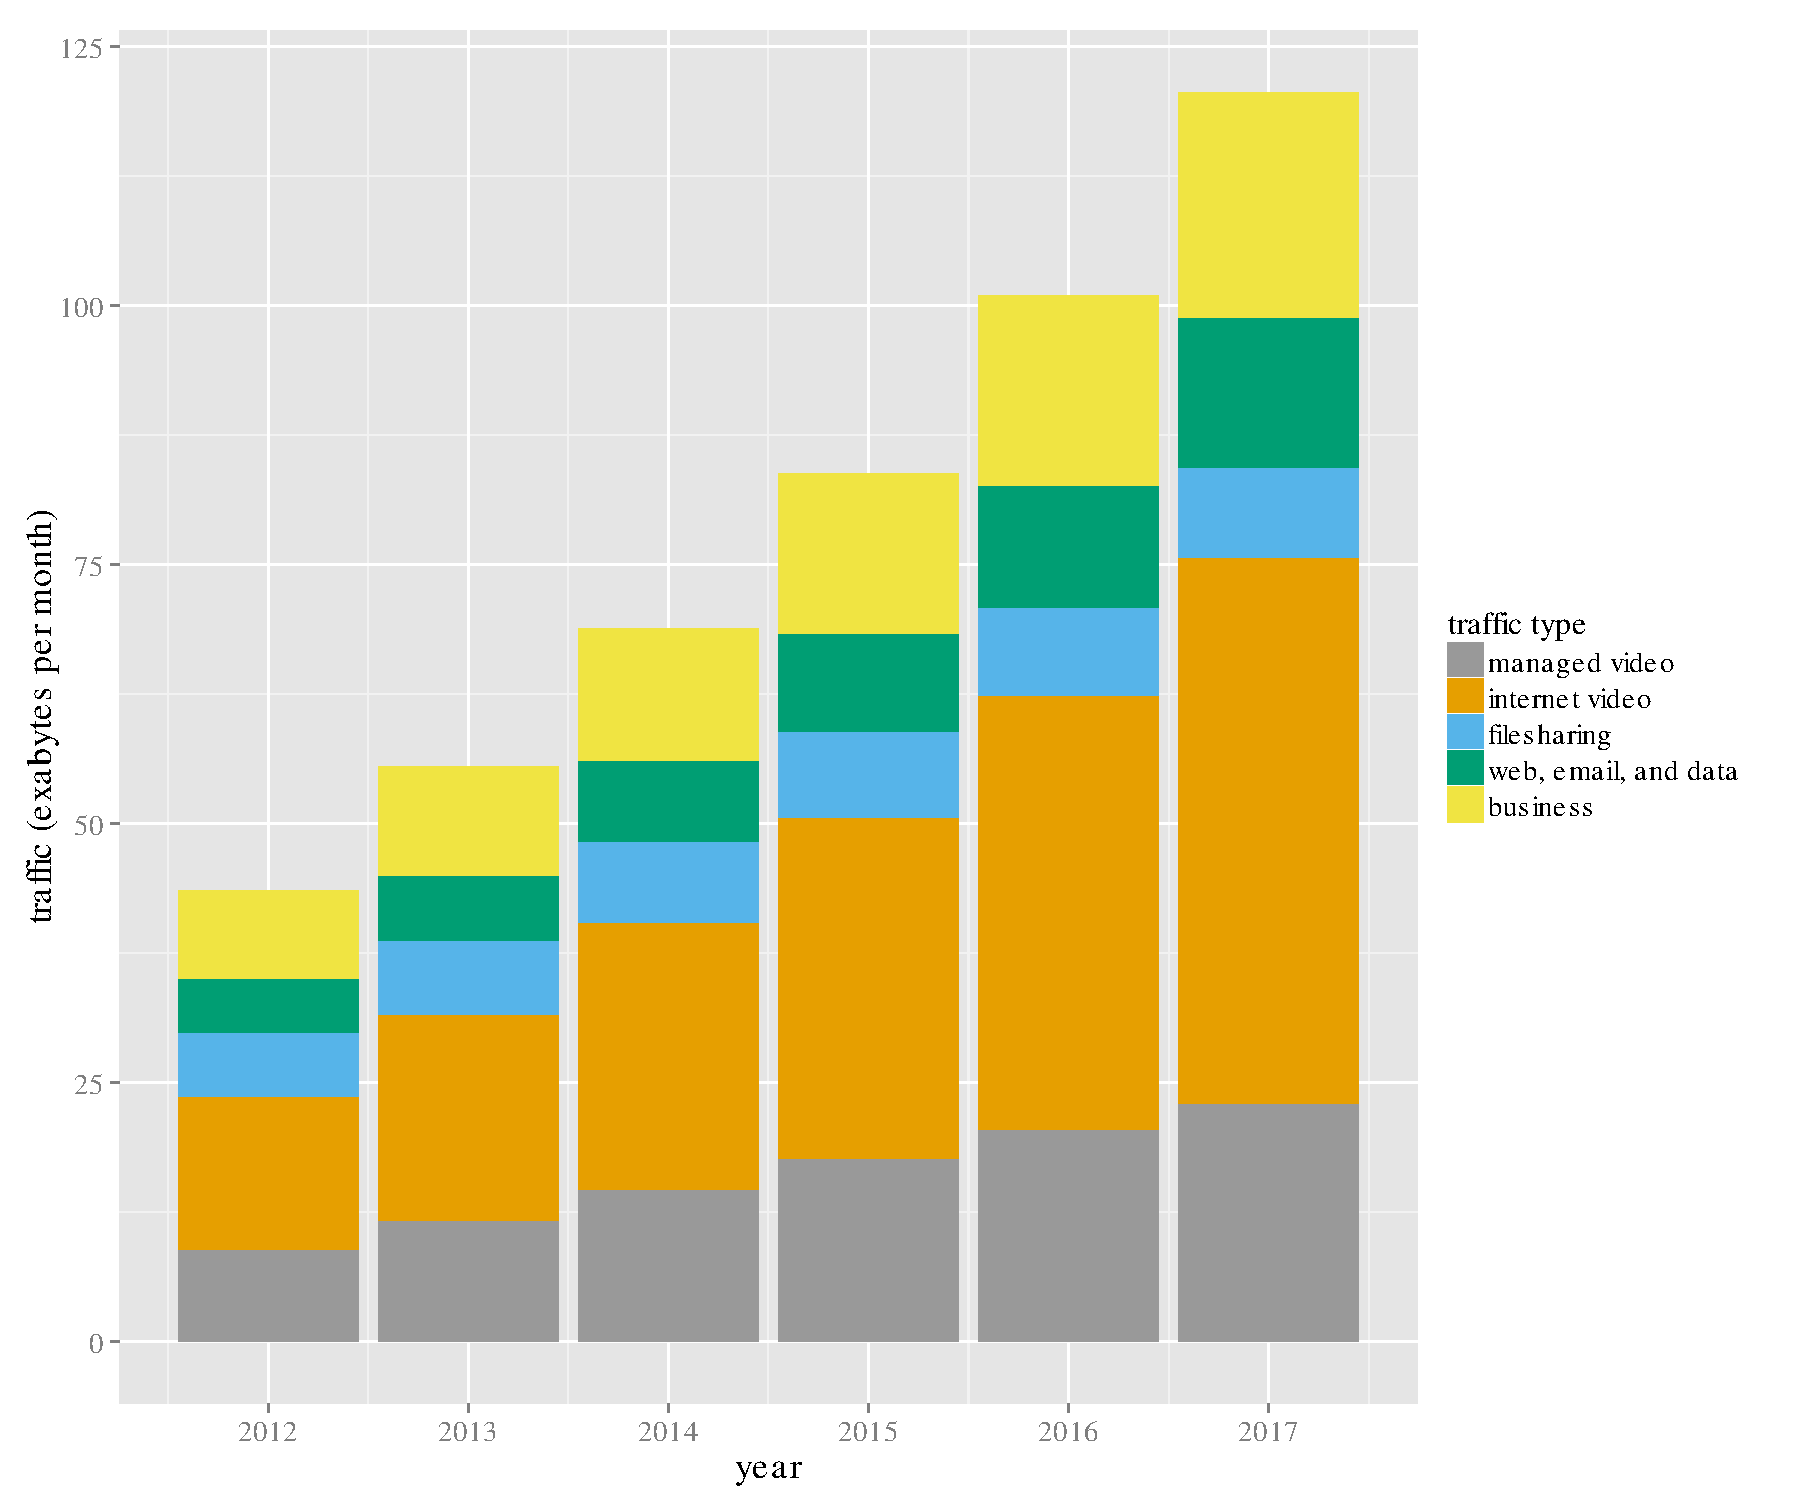
\includegraphics[height=6cm]{../../chapters/01-intro/images/r-cisco-vni-2013.pdf}
		\caption{Cisco's global consumer Internet traffic prediction (data source:~\cite{cisco2013VNI}).}
	\end{figure}
\end{frame}


\begin{frame}
    \frametitle{Introduction}
    \framesubtitle{And Reliable Streaming in Mobile Networks?}

    \begin{columns}[T]
    	\begin{column}[T]{5cm}
			\begin{figure}
				\centering
				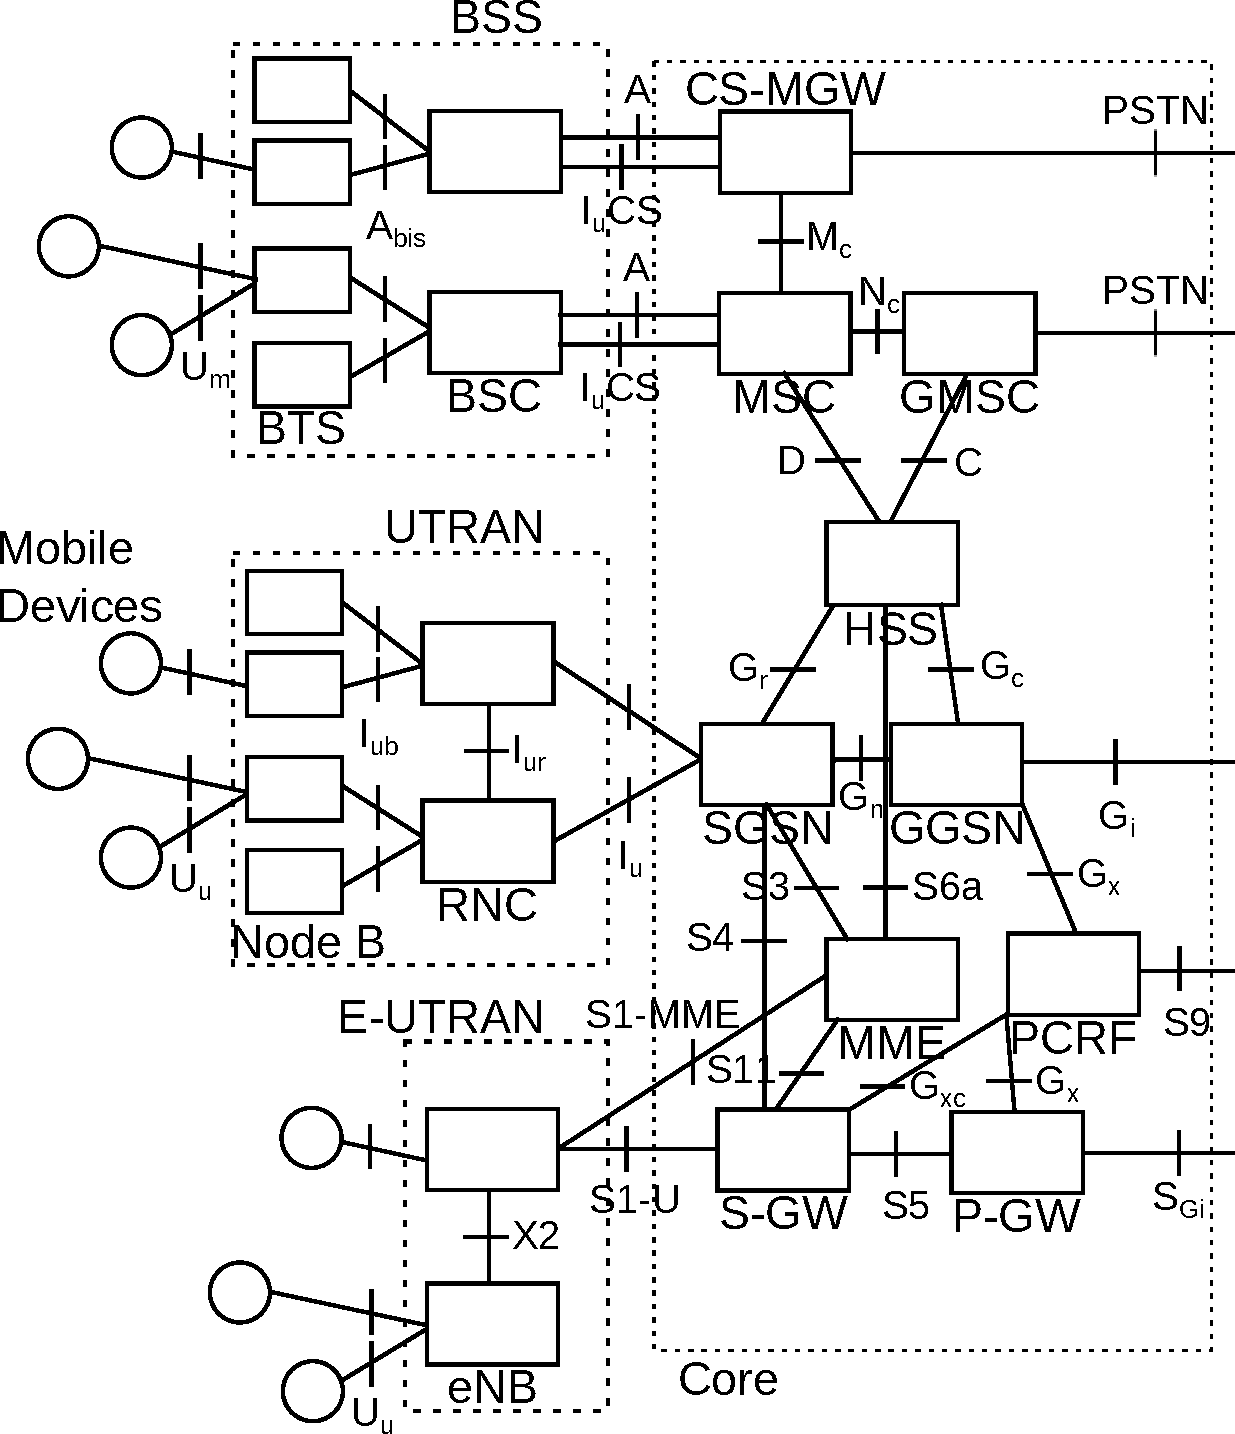
\includegraphics[height=6cm]{../../chapters/04-mobilenets/images/3gpp-physical-arch.pdf}
				%\caption{Overview of a combined CS/PS GSM/UMTS/LTE architecture.}
			\end{figure}
		\end{column}

		\begin{column}[T]{5cm}
			\begin{figure}
				\centering
				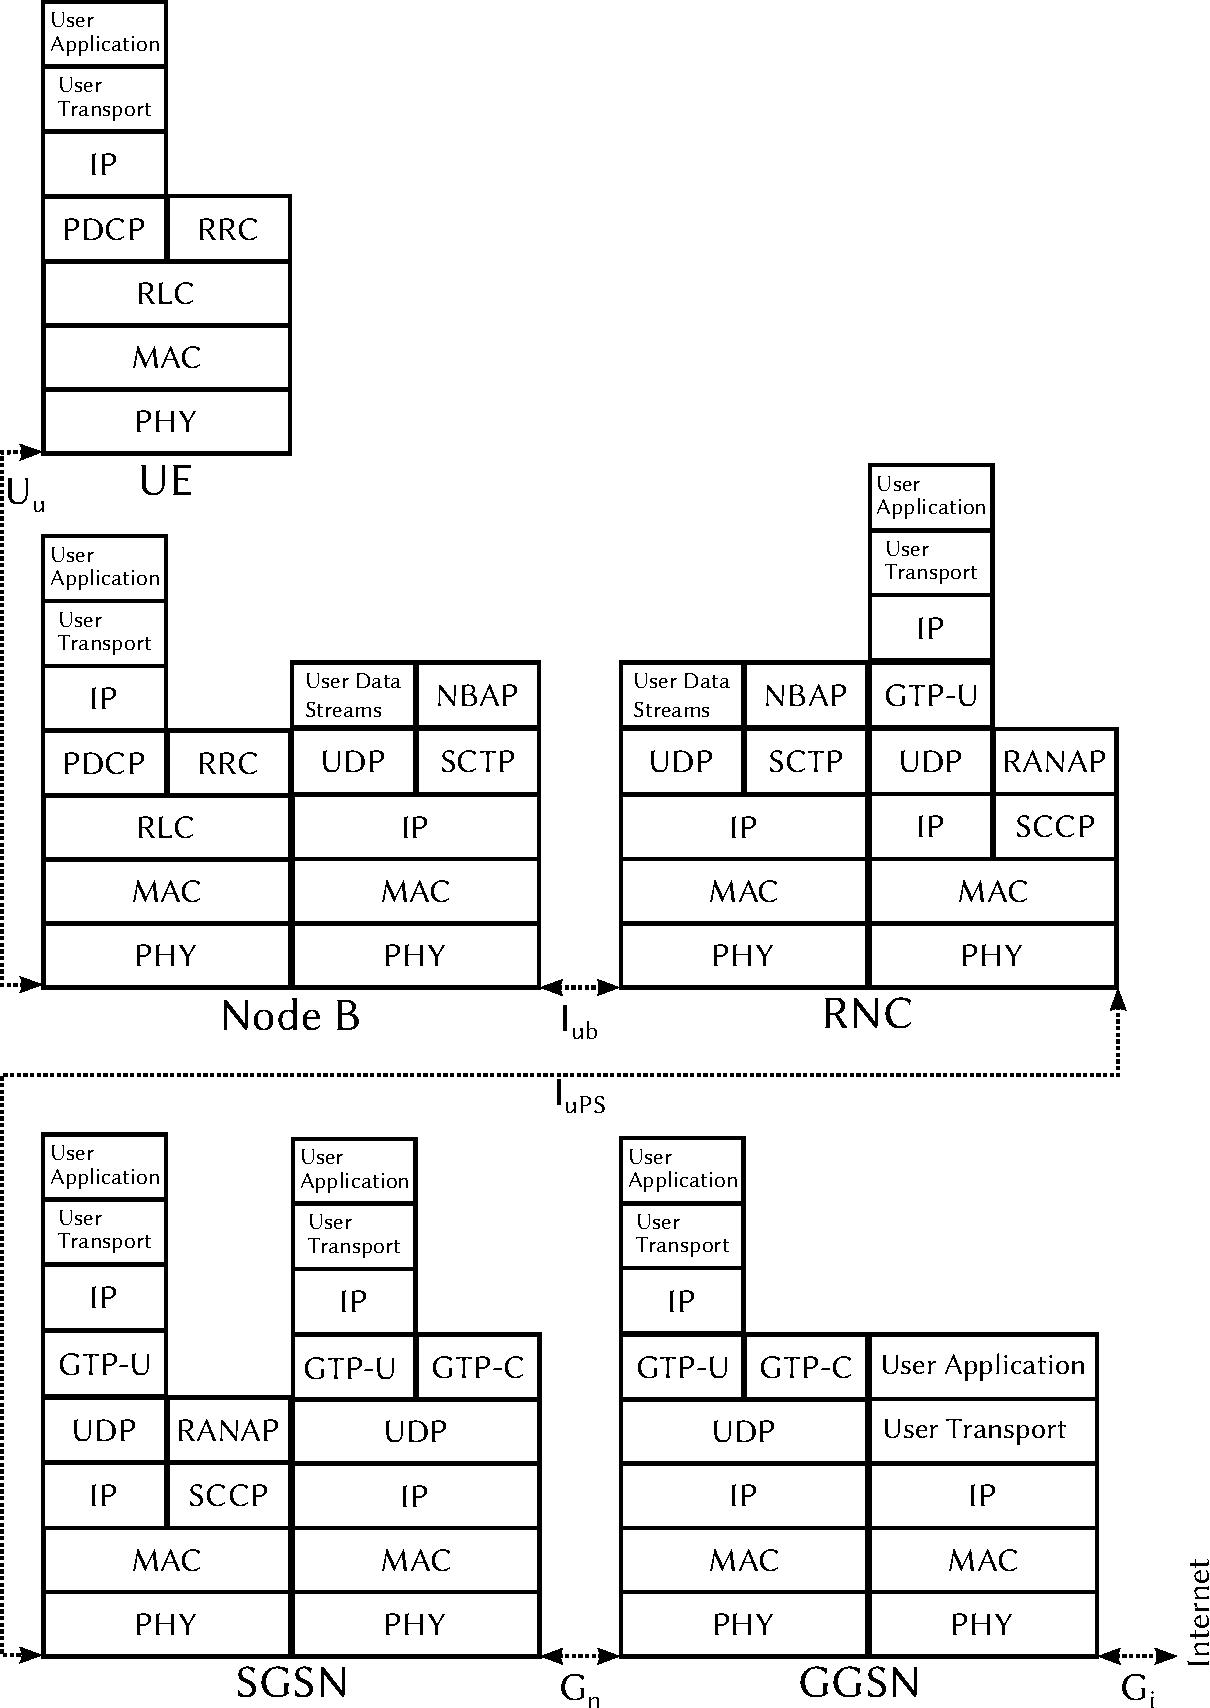
\includegraphics[height=6cm]{../../chapters/04-mobilenets/images/umts-userpath-stack.pdf}
				%\caption{Simplified control plane and user plane IP-based protocol stacks on the user traffic path through the mobile network.}
			\end{figure}
		\end{column}
	\end{columns}
	\pause

	\Put(85,200){\color{blue}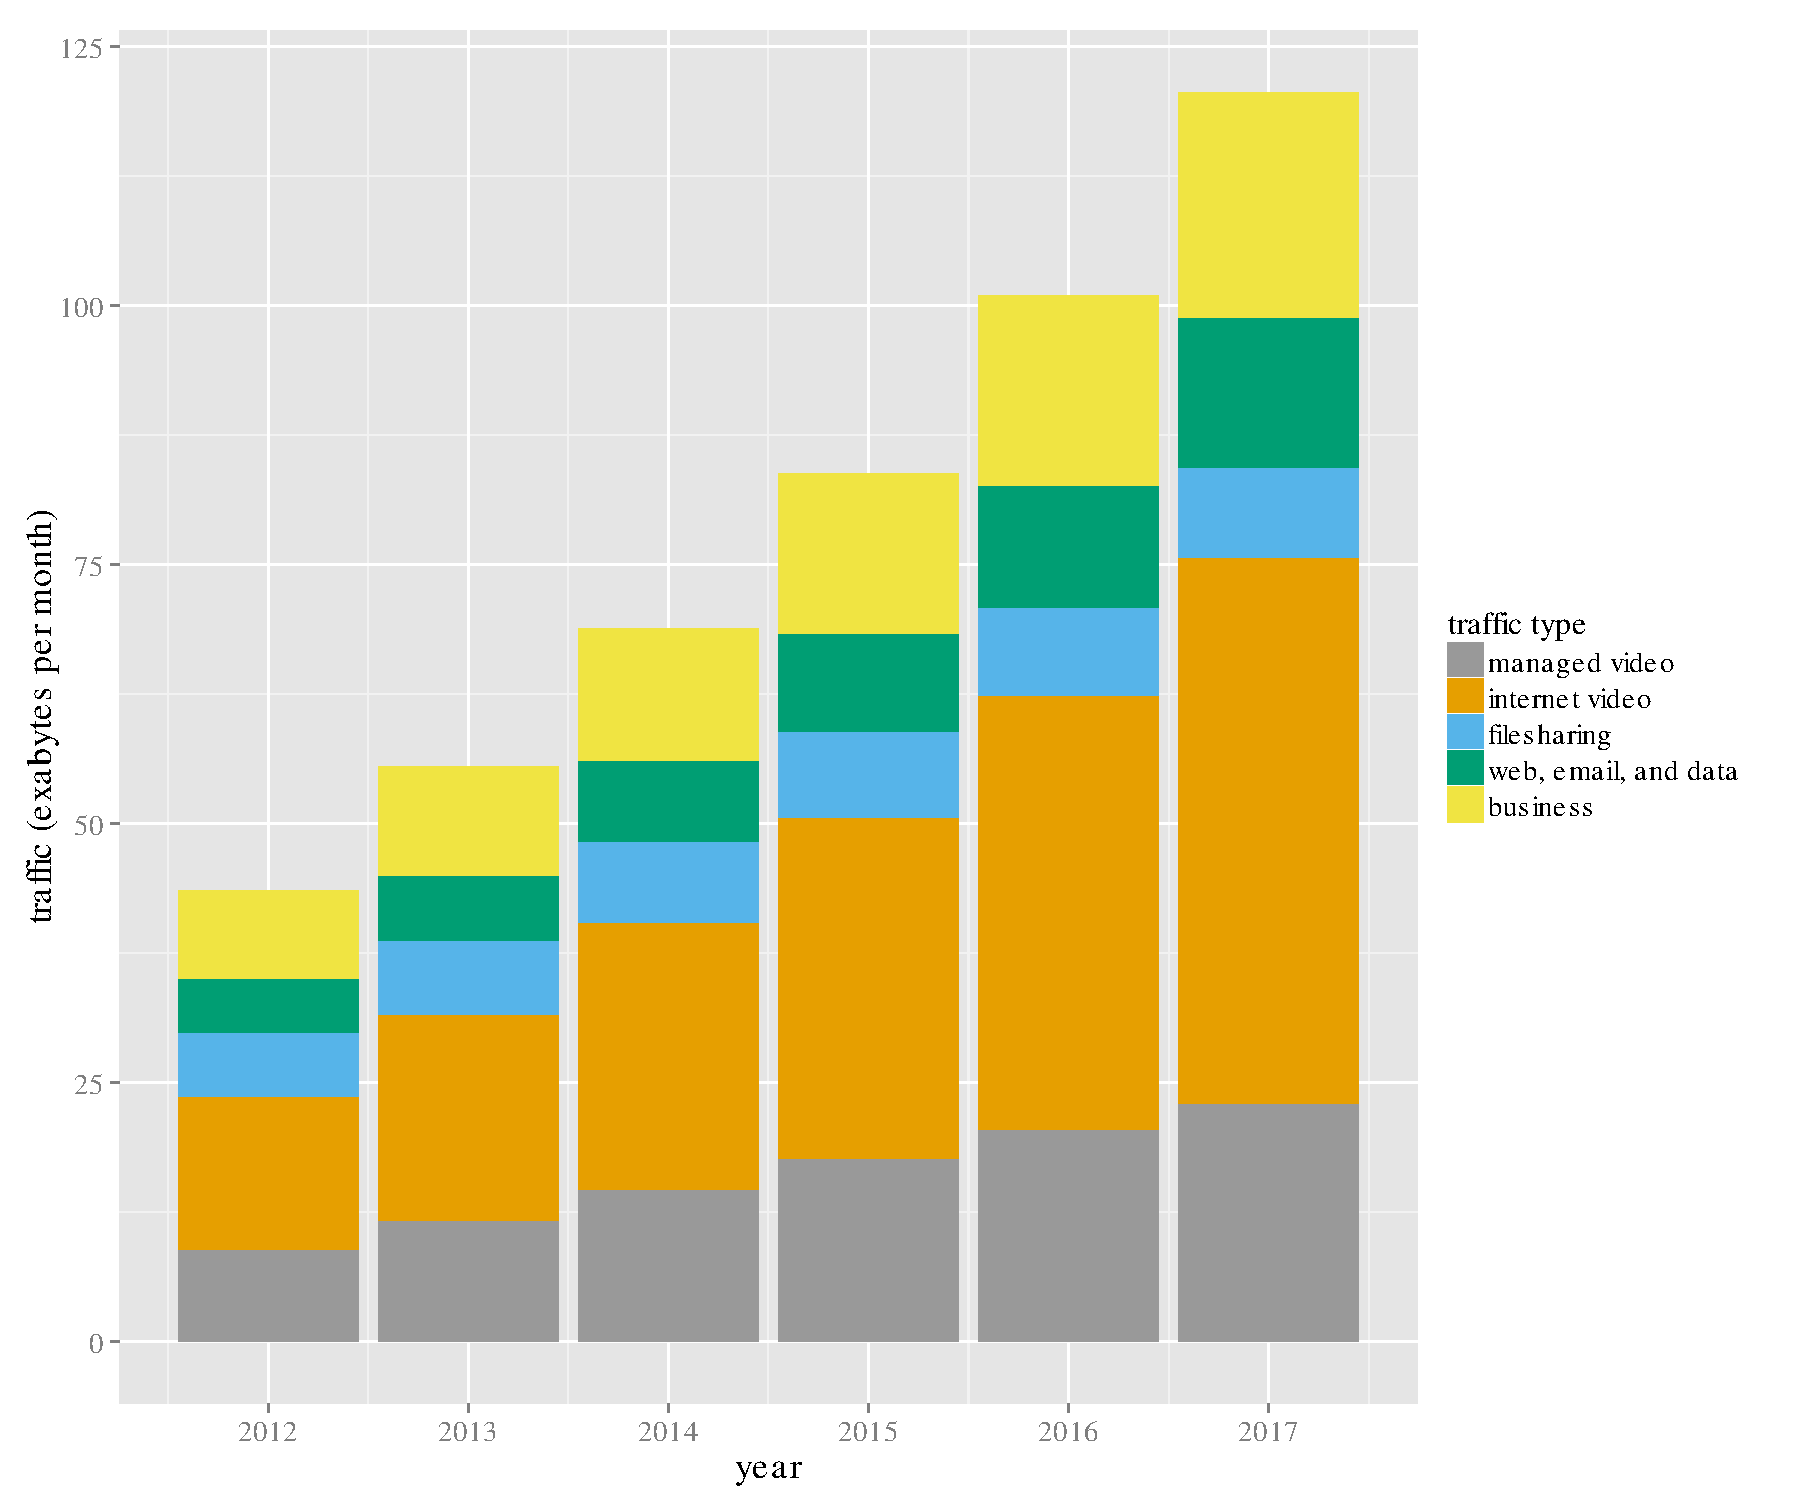
\includegraphics[height=4cm]{../../chapters/01-intro/images/r-cisco-vni-2013.pdf}}
\end{frame}


\begin{frame}
	\frametitle{Introduction}
	\framesubtitle{Current State of Affairs}

	\begin{itemize}
		\item Reliable streaming largely supplants RTP/UDP streaming in the Internet
		\item Mobile network traffic share increasing rapidly
		\item What about the influence of the mobile core network and control plane?
		\item What makes reliable streaming that different from previous approaches?
		\item Interaction between reliable streaming and mobile control plane?
		\item How to properly measure and model these circumstances?
	\end{itemize}

	\begin{itemize}[<2->]
		\item From passive measurements derive a CN control plane load model
		\item Categorize and present a model for reliable streaming measurements
		\item Discuss influence factors on reliable streaming
		\item Present mobile streaming measurement approaches
	\end{itemize}
\end{frame}


\begin{frame}
	\frametitle{Introduction}
	\framesubtitle{Thesis Structure}

	Thesis consists of two intersecting angles
	\begin{enumerate}
		\item Evaluation of a 3G core network
			\begin{itemize}
				\item Investigation and evaluation of the control plane
				\item Modeling and simulating load
			\end{itemize}

		\item Investigation of TCP-based video streaming techniques
			\begin{itemize}
				\item Protocol survey and classification
				\item Deriving a model
				\item Measurements with the model
			\end{itemize}

		\item Measuring video streaming in a 3G network 
			\begin{itemize}
				\item Investigation of influence factors and countermeasures
				\item Comparison of investigation approaches (active measurements and simulation)
			\end{itemize}
	\end{enumerate}


	% \begin{block}{}
	% 	This presentation
	% \end{block}
\end{frame}






%%%%%%%%%%%%%%%%%%%%%%%%%%%%%%%%%%%%%%%%%%%%%%%%%%%%%%%%%%%%%%%%%%%%%%%%%%%%%%%%
\section{Mobile Core Network Architecture}
%%%

\begin{frame}
	\frametitle{Core Network and Control Plane Overview}


    \begin{columns}[T]
    	\begin{column}[T]{5cm}
			\begin{itemize}
				\item Looking at UMTS/3G in particuar, but GSM/GPRS almost the same
				\item LTE with certain updates to architecture
					\begin{itemize}
						\item SGW/PGW instead of SGSN/GGSN
						\item but mostly similar protocols/procedures
						\item not further mentioned
					\end{itemize}

				\item Everything is connected (cross-node, cross-layer)
					\begin{itemize}
						\item Action at mobile device will trigger procedures deep inside the network
					\end{itemize}

				%\item tunnel management signaling: creation, deletion, and update request/response messages
			\end{itemize}
		\end{column}

    	\begin{column}[T]{5cm}
			\begin{figure}
				\centering
				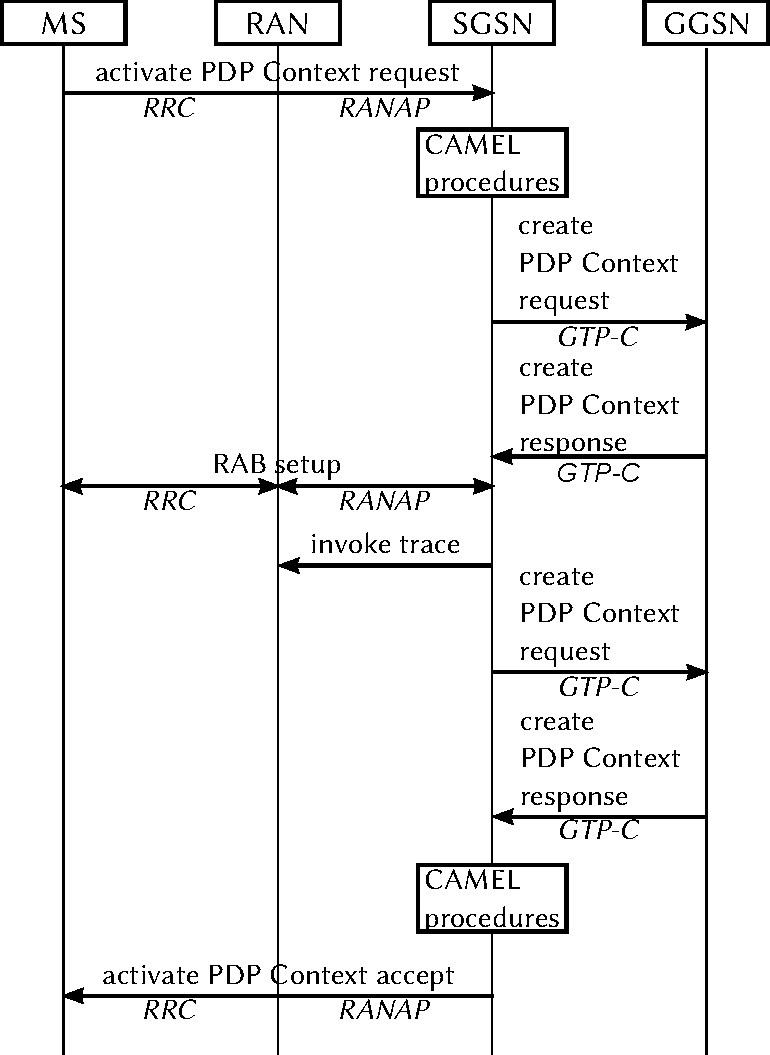
\includegraphics[height=6cm]{../../chapters/04-mobilenets/images/pdp-context-activation-procedure.pdf}
			\end{figure}
			\vspace{-0.5cm}
			{\small PDP Context activation procedure}
		\end{column}
	\end{columns}
\end{frame}


\begin{frame}
    \frametitle{GTP Tunneling Concept}

    \begin{itemize}
		\item Any user traffic in a 3G net is encapsulated into tunnels
		\begin{itemize}
			\item Radio bearer to the device
			\item GPRS Tunneling Protocol (GTP) at L4 used between SGSN and GGSN
		\end{itemize}
		\item Tunnel state (PDP Context) held at and signaled/synchronized between core nodes through create/delete/update request/response pairs
		\item Imposes certain overhead and load onto the network
		\begin{itemize}
			\item Network: through signaling messages and additional headers
			\item Memory: keeping track of state for every tunnel (``PDP Context'')
			\item CPU: tracking state changes and processing tunnel requests
		\end{itemize}
	\end{itemize}

	\begin{columns}
		\column{0.5\textwidth}
			\vspace{-0.6cm}
			\begin{figure}	
				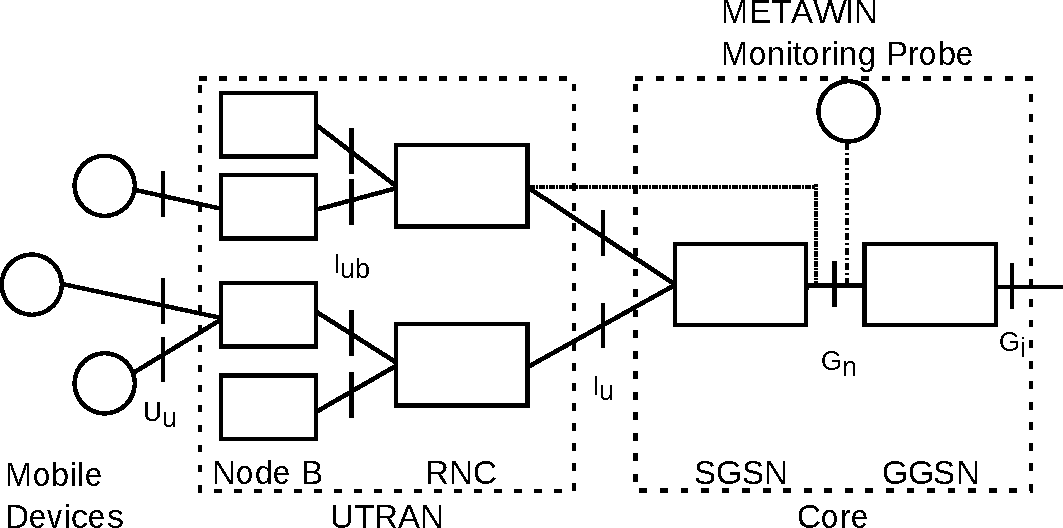
\includegraphics[height=2.5cm]{../../chapters/04-mobilenets/images/umts-network.pdf}
			\end{figure}

		\column{0.5\textwidth}
			\vspace{-0.6cm}
			\begin{figure}
				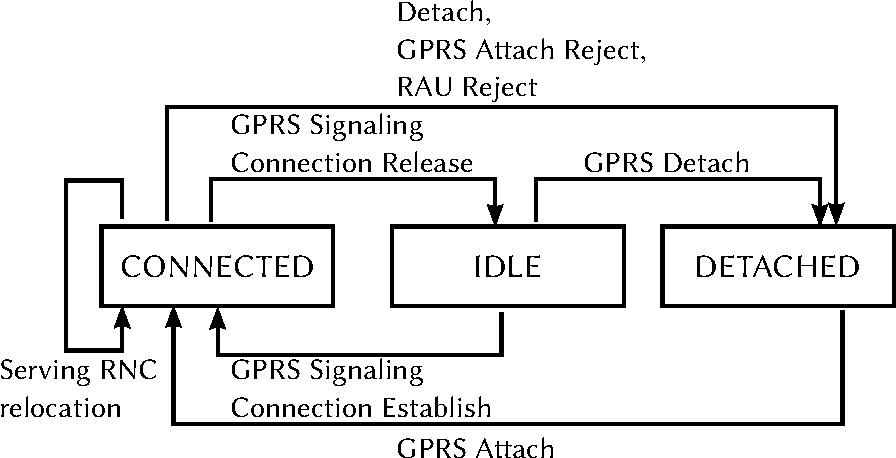
\includegraphics[height=2.5cm]{../../chapters/04-mobilenets/images/mm-3g-state-model.pdf}
			\end{figure}
			%\vspace{-0.5cm}
			%{\centering\small SGSN MM state machines}
	\end{columns}
\end{frame}



\begin{frame}
	\frametitle{Mobile Network Load}
	
	Definitions
	\begin{itemize}
		\item Most commonly defined as direct user traffic load
			\begin{itemize}
				\item control plane signaling often not factored in
			\end{itemize}

		\item Factor in control plane and core network
			\begin{itemize}
				\item For one node $n$: $\rho_{n} = \max(\rho_{l,n}, \rho_{m,n}, \rho_{p,n})$ (link load $\rho_{l}$, memory load $\rho_{m}$, processing load $\rho_{p}$)
				\item total load of the core: $\rho_{CN} = \max_{n \in CN}(\rho_{n})$
				\item one factor at one node will be the bottleneck
			\end{itemize}
	\end{itemize}


	Reasoning for GGSN as load bottleneck
	\begin{itemize}
		\item single instance responsible for whole (or complete region) network
		\item handles PDP Context Management signaling, PDP Context state for each device and tunnel
		\item involved in almost all network-wide signaling procedures
		\item GTP Mobility Management signaling from SGSN
	\end{itemize}

%\item link load: ratio of the used versus the available bandwidth on a link $\rho_{l} = \frac{b_{u}}{b_{a}}$
		%\item network load: average load of all involved links $\rho_{N} = \frac{\sum_{i \in N} \rho_{l,i}}{|N|}$
		%\item mobile core network node load: $\rho_{n} = \max(\rho_{l,n}, \rho_{m,n}, \rho_{p,n})$ 	with the memory load $\rho_{m}$ and processing load $\rho_{p}$

\end{frame}



\begin{frame}
	\frametitle{Load Influencing Factors}
	Many sources of influence, both internal as well as external

	Network-centric factors
	\begin{itemize}
		\item Specific interaction of state machines and protocols
		\item Inactivity timers (e.g. moving device from connected to idle/detached)
	\end{itemize}

	\vspace{0.3cm}
	
	User-centric factors
	\begin{itemize}
		\item Type and OS of device, access technology
		\item Installed and active applications
		\item Specific usage, time-of-day, and traffic patterns
		\item Restrict to features identifiable from a network perspective
	\end{itemize}

	\vspace{0.3cm}

	\only<2->{Load evaluation approach}
	\begin{itemize}[<2->]
		\item Investigate load at \textbf{GGSN}
		\item Do this on the basis of \textbf{GTP tunnel characteristics}
	\end{itemize}

\end{frame}




%%%%%%%%%%%%%%%%%%%%%%%%%%%%%%%%%%%%%%%%%%%%%%%%%%%%%%%%%%%%%%%%%%%%%%%%%%%%%%%%
\section{Evaluating Mobile Signaling Traffic and Load}
%%%


\begin{frame}
	\frametitle{Trace Evaluation}
	Recorded dataset
	\begin{itemize}
		\item One week long passive measurements in an operator's core network (METAWIN, April 2011)
		\item 2.2Bn user traffic records, 410M GTP tunnel management messages
		\item Trace data not raw, but anonymized and reduced to select fields per signaling interactions
		\item Limits evaluation possibilities 
	\end{itemize}

	\only<2->{Device identification}
	\begin{itemize}[<2->]
		\item Individual devices trackable through pseudonymized IMSI/IMEI
		\item Device type distinguishable through type allocation code (TAC)
		\item No free TAC-to-device mappings available, mappings collected manually
		\item Manual mapping covers \SI{80.93}{\percent} of distinct devices and \SI{87.57}{\percent} of tunnels in the dataset
		\item TAC also allows (partial) differentiation of the OS (e.g. Android and iOS)
	\end{itemize}
\end{frame}


\begin{frame}
	\frametitle{Trace evaluation}

	Initial findings
	\begin{itemize}
		\item Link load of control traffic insignificant
			\begin{itemize}
				\item GTP messages contribute estimated upper limit of \SI{0.7}{\percent} to total traffic
			\end{itemize}
		\item Significant portion of devices (\SI{18}{\percent}) that causes signaling traffic without transmitting any user traffic
		\item Causing high amounts of user traffic does not lead to a high amount of signaling messages
			\begin{itemize}
				\item E.g. 3G dongles responsible for \SI{75}{\percent} of traffic, but only \SI{10}{\percent} of GTP signaling messages
			\end{itemize}
	\end{itemize}

	\only<2->{Next steps}
	\begin{itemize}[<2->]
		\item Build a queuing theory model for GTP tunnels at the GGSN
		\item Closely investigate tunnel arrival and service process
		\item Derive distributions for these processes
	\end{itemize}
\end{frame}


\begin{frame}
	\frametitle{Tunnel Arrivals}
	\framesubtitle{By Time of Day}
		%\framesubtitle{Interarrival Time of Successful Tunnel Requests}
	\begin{columns}[T]
		\column{.5\textwidth}
			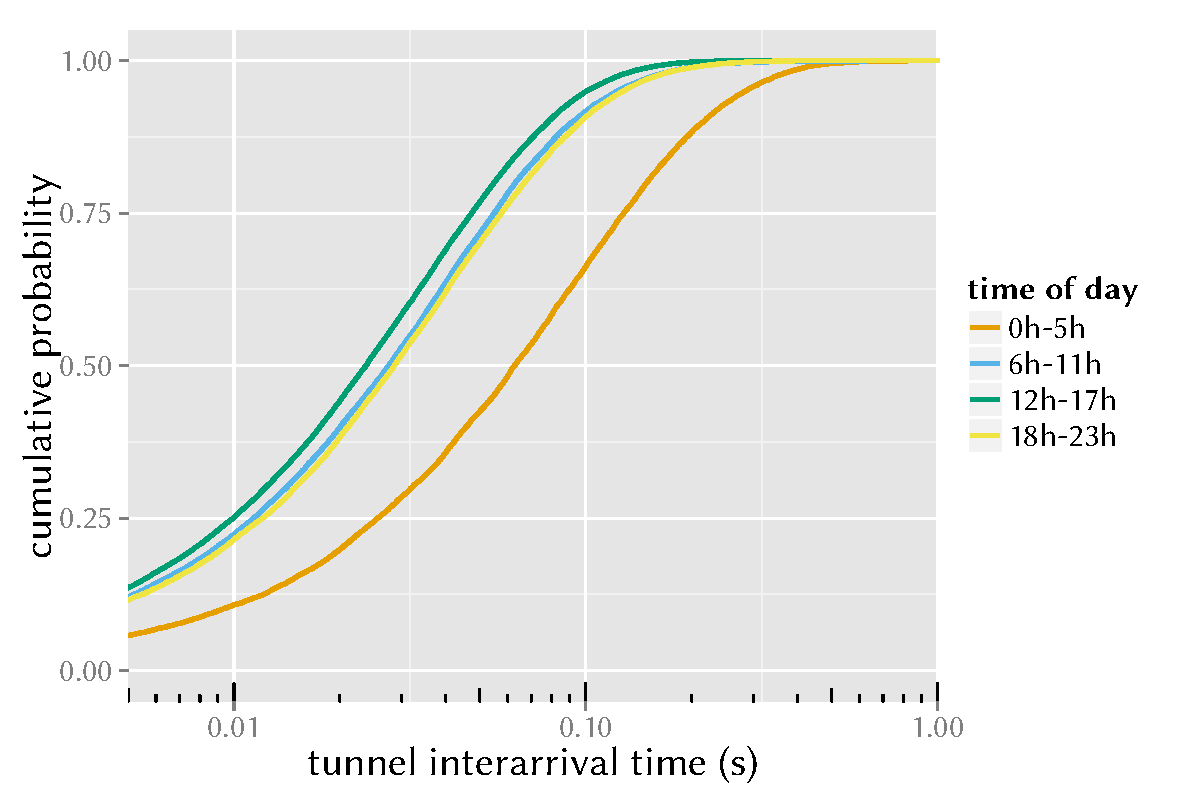
\includegraphics[width=1.0\columnwidth]{../../chapters/041-mobilenetsmeasuring/images/R-IAT-fromflows-ecdfs-2h.pdf}

		\column{.5\textwidth}
			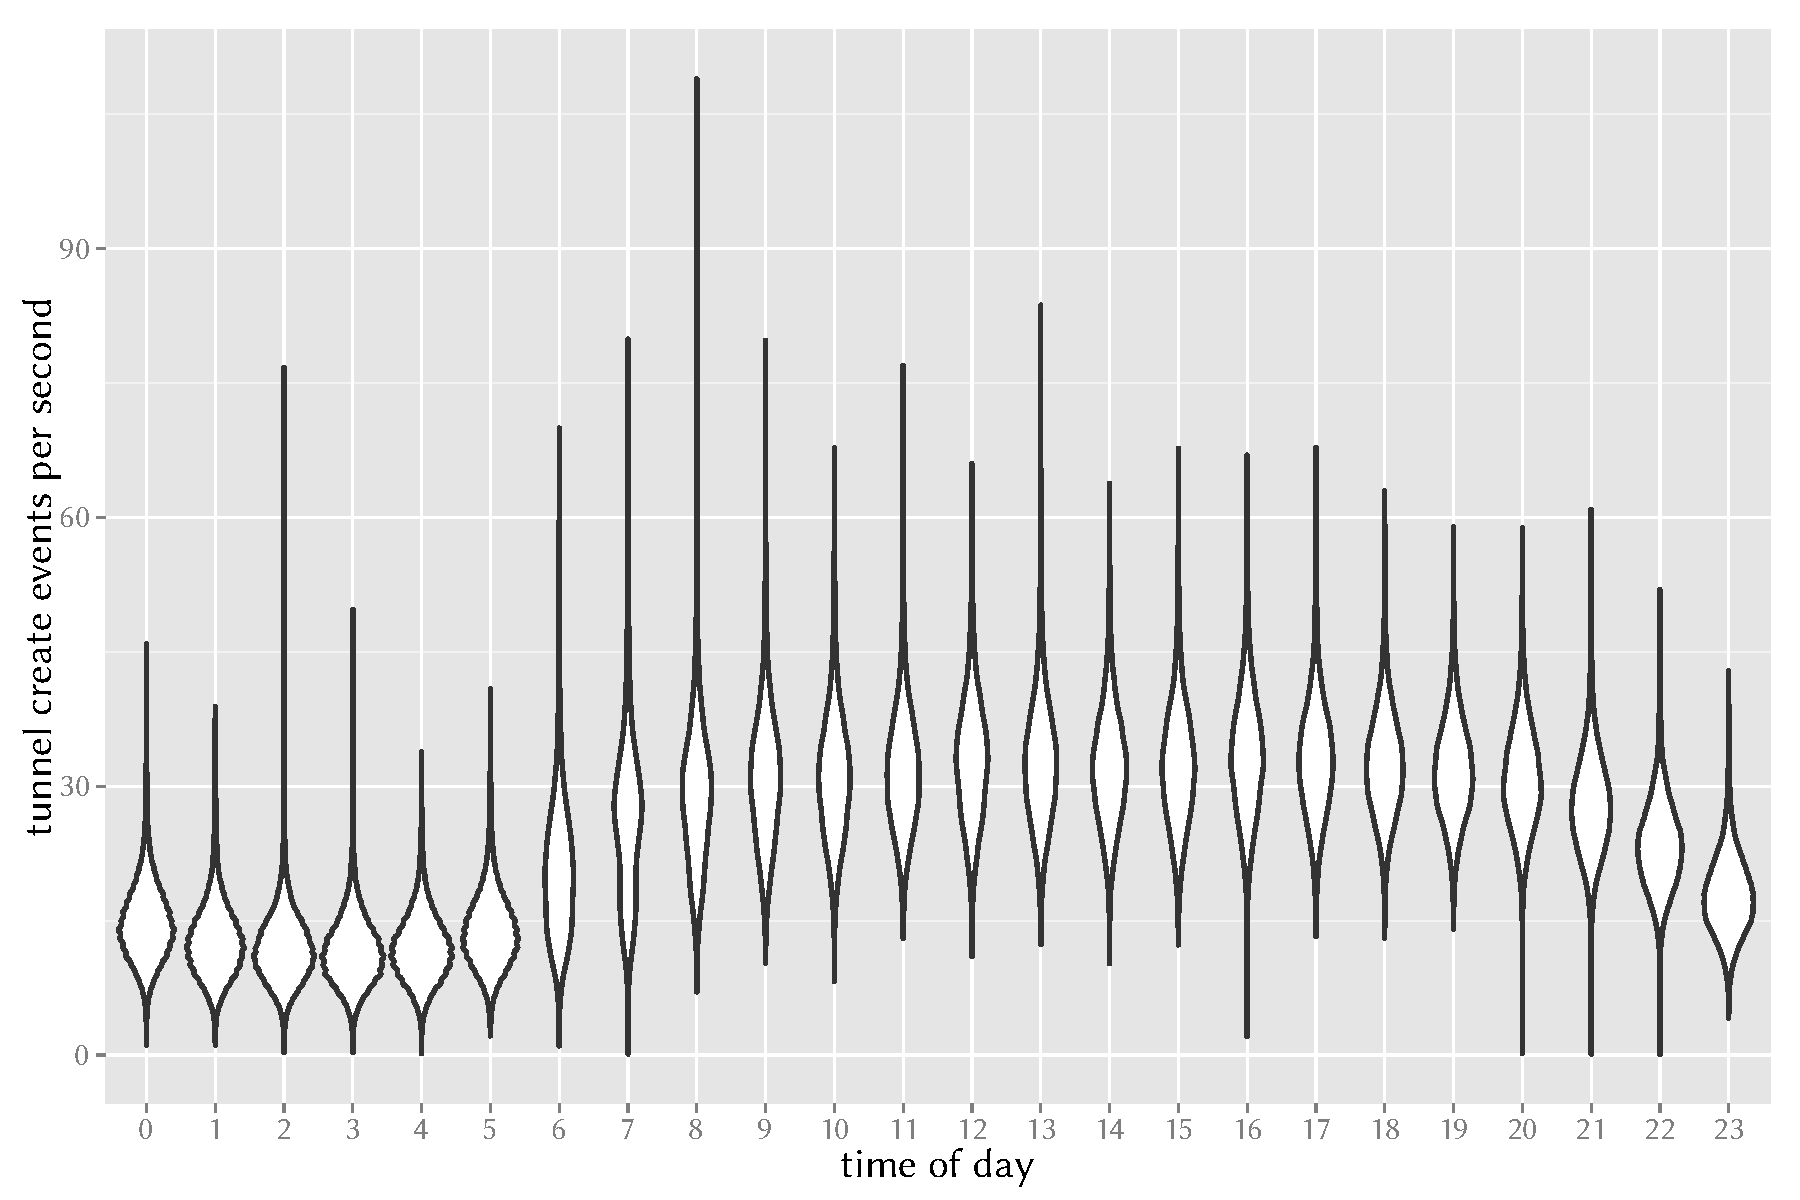
\includegraphics[width=1.0\columnwidth]{../../chapters/041-mobilenetsmeasuring/images/R-createspersecond-1h-violin.pdf}
	\end{columns}

	\begin{itemize}
		\item Strong time of day dependence with busy hour in the early afternoon
		\item Bimodal character of arrival rate over the total time of day
	\end{itemize}
\end{frame}



\begin{frame}
	\frametitle{Tunnel Durations}

	\begin{columns}[T]
		\column{0.5\textwidth}
			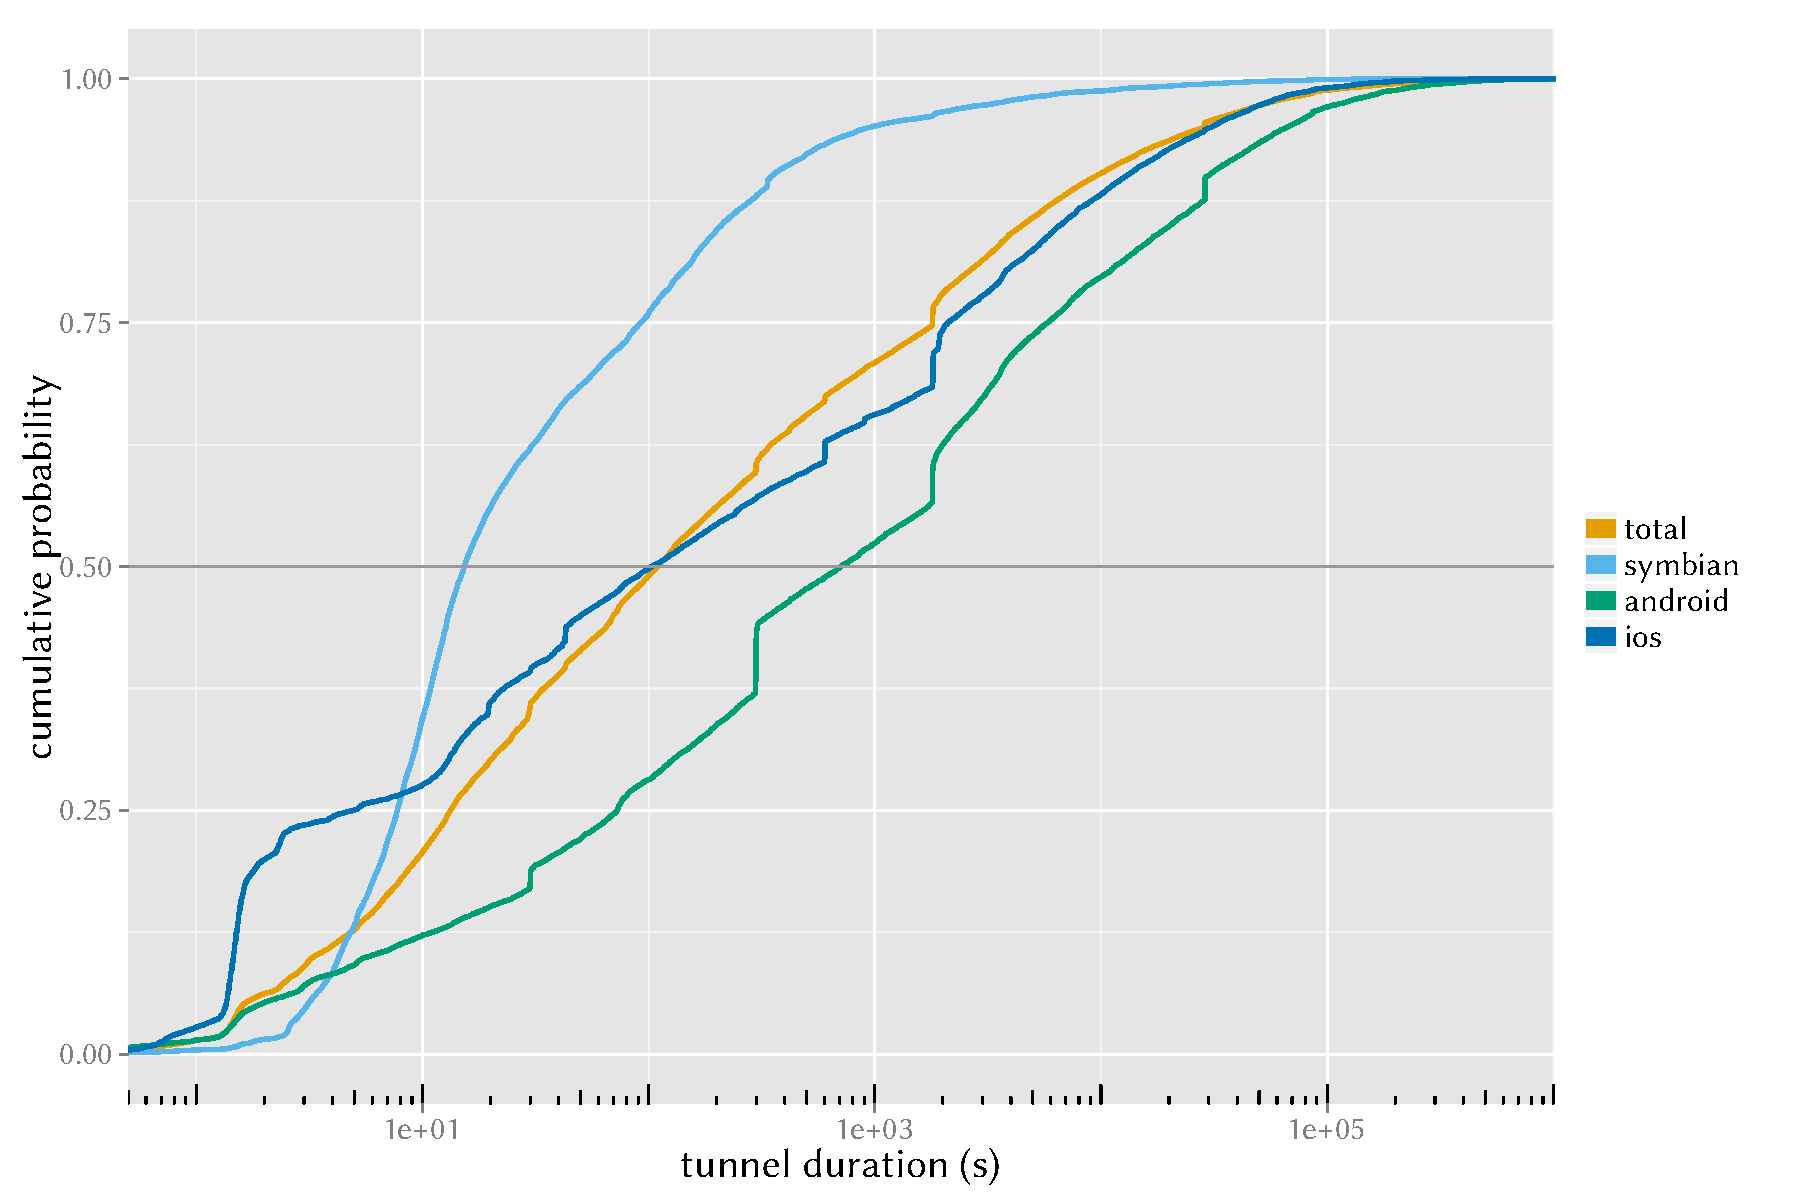
\includegraphics[width=\columnwidth]{../../chapters/041-mobilenetsmeasuring/images/R-tunnel-duration-operating-system.pdf}

		\column{0.5\textwidth}
			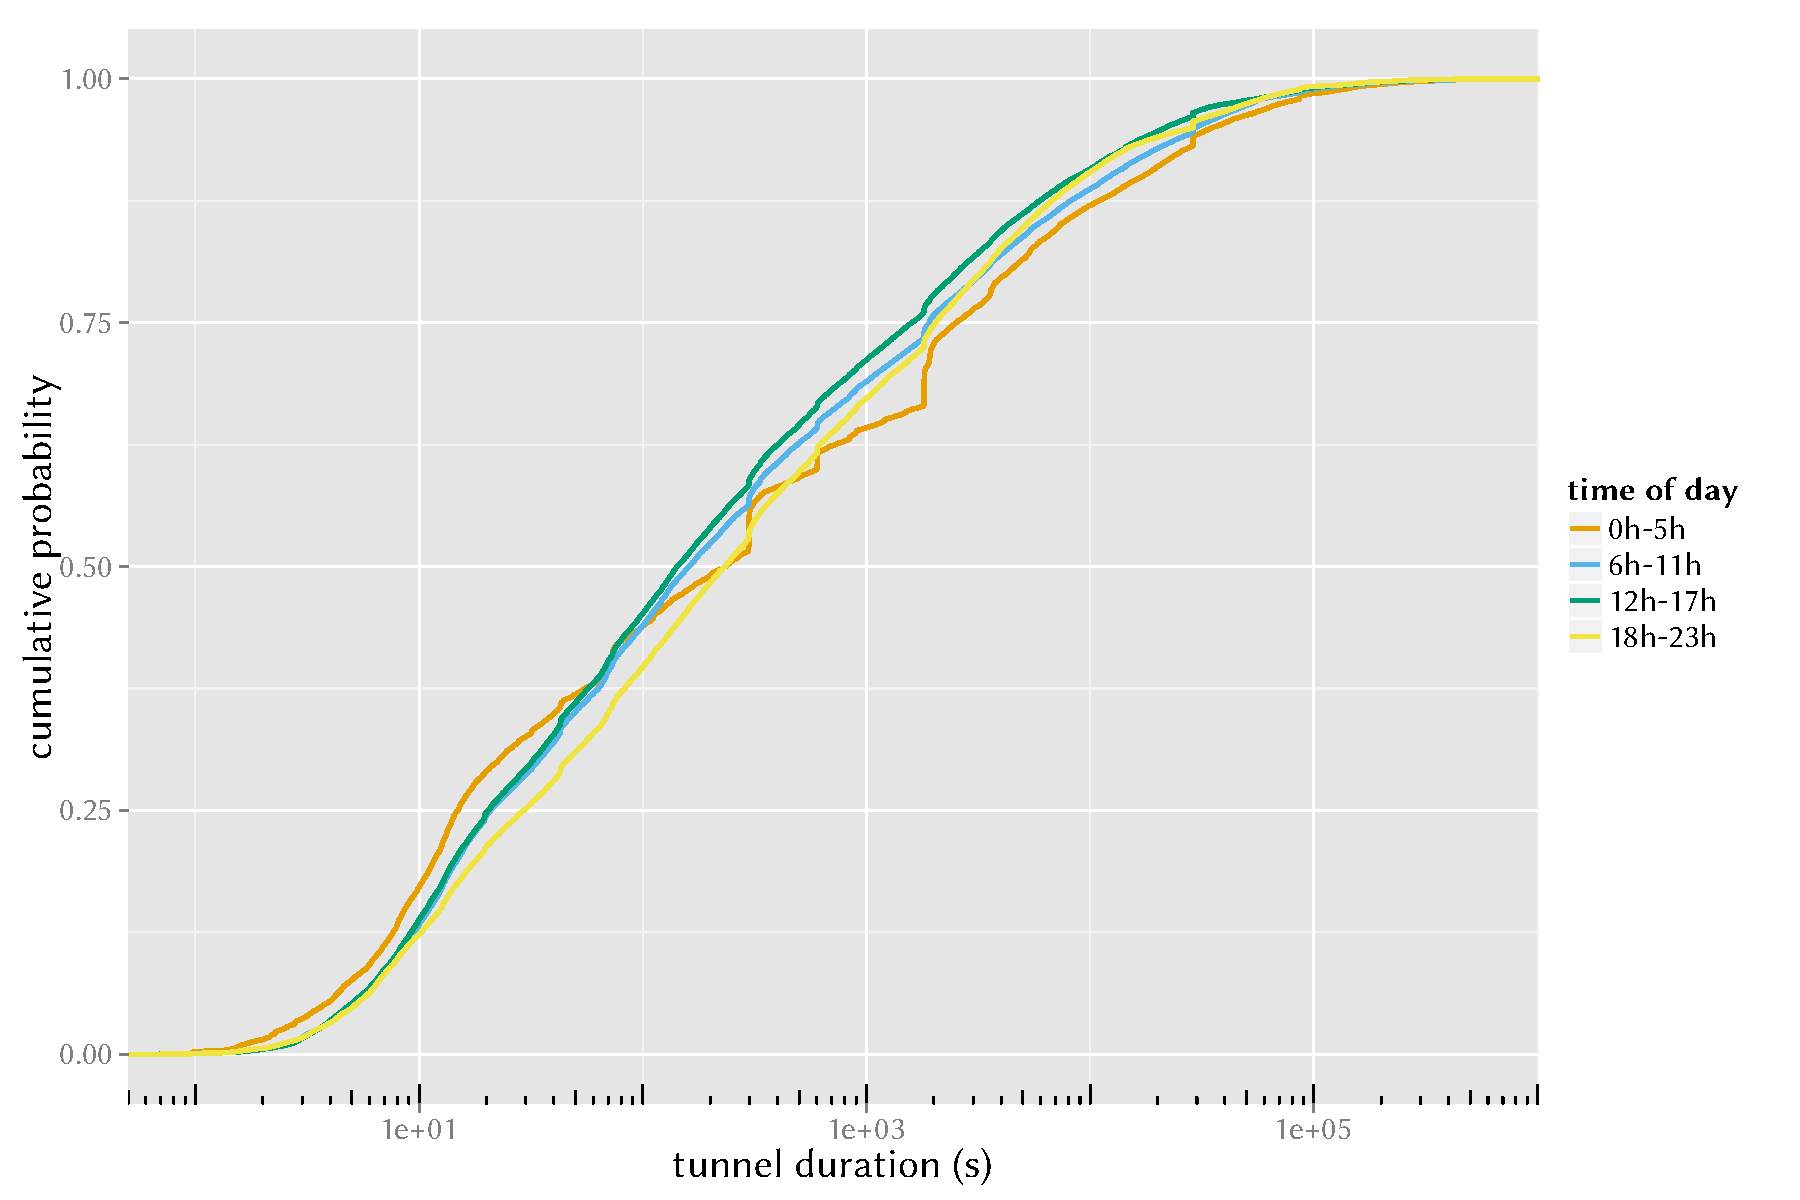
\includegraphics[width=\columnwidth]{../../chapters/041-mobilenetsmeasuring/images/R-duration-timeofday-ecdf.pdf}
	\end{columns}

	\begin{itemize}
		\item Only slight dependence on time of day
		\item Much stronger influence of user device type, OS, or network timers
		\item Phenomenon sometimes discussed as ``signalling storm'' visible here (in the core network, not just radio!)
	\end{itemize}
\end{frame}



%%%
%\subsection{Models}
%%%


\begin{frame}
	\frametitle{Deriving a Model}
	\framesubtitle{Monolithic GGSN Queuing Model}
		\begin{center}
			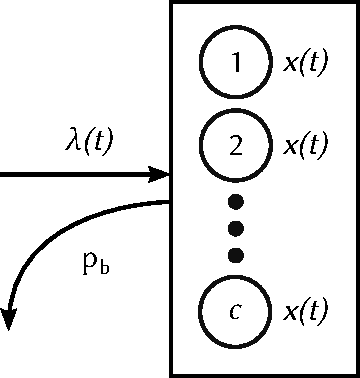
\includegraphics[height=3cm]{../../chapters/041-mobilenetsmeasuring/images/ggsn-monolithic.pdf}
		\end{center}

		\begin{itemize}
			%\item Fit the time-of-day-differentiated arrival and serving processes
			\item Poisson tunnel arrival process with rate $\lambda(t)$ fitted with trace data
			\item GGSN can serve $n$ tunnels in parallel, limited by network/processing load and signaling/state overhead
			\item Tunnel duration $x(t)$ as general distribution, fitted with rational function
			\item If GGSN is full, reject new tunnels, leads to blocking probability $p_b$
			\item[$\rightarrow$] Non-stationary Erlang loss model $M(t)/G(t)/c/0$ 
		\end{itemize}

\end{frame}


\begin{frame}
	\frametitle{Expanding the Model}
	\framesubtitle{Virtualized GGSN Queuing Model}
		\begin{center}
			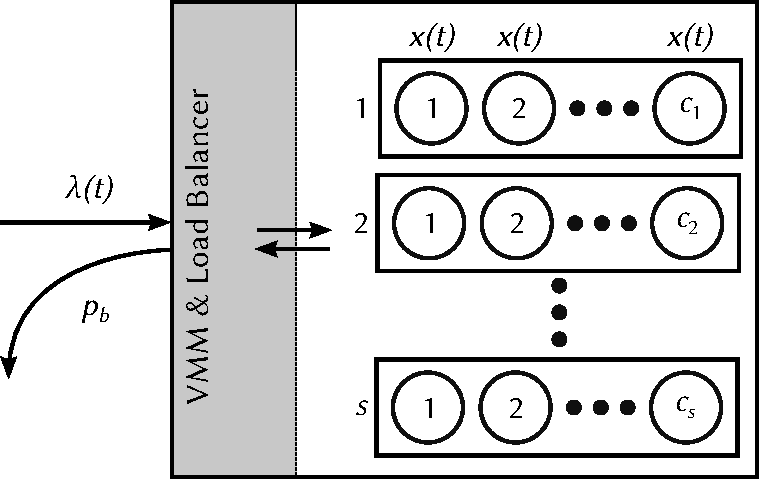
\includegraphics[height=3.5cm]{extras/ggsn-virtualized.pdf}
		\end{center}

		\begin{itemize}
			\item Suggestion for improvement over the current monolithic status quo
			\item Same arrival and serving time process, no queue
			\item Load balancing strategies for VM management and tunnel placement
			%Hypervisor distributes tunnels and starts on demand up to $s_{max}$ virtualized GGSN instances, each with capacity $m$
			%\item Up to $s_{max}$ instances with capacity of $m$ each
			%\item Instance count kept near actual system load (energy efficiency)
			\item Can incur additional blocking (virtualization overhead)
			% when new instances are not switched on fast enough, or instance overhead if not shut down when unused
			\item Additional dimension for scaling compared to monolithic model
			\item[$\rightarrow$] $M(t)/G(t)/\|\overrightarrow{c}\|_1/0$ % 1-norm des Kapazitätsvektors
		\end{itemize}
\end{frame}


%%%
\subsection{Queuing Simulation}
%%%


\begin{frame}
	\frametitle{Model Evaluation/Simulation}

	\begin{itemize}
		\item No tractable analytic solution for $M(t)/G(t)/c/0$ models
		\item Use queuing simulation with the fitted distributions
		\item SimPy3-based DES, one week period, 10 repetitions, naive VMM
		\item Variables: Total tunnel capacity, number and capacity of VMs
		\item Evaluate blocking probability and VM usage
		%\item Arrival process with exponential distributions fitted to dataset, four time of day slots
		%($\lambda=\{10.67,24.53,29.25,23.50\}$ before normalization)
		%\item Tunnel duration CDF fitted with a rational function
		%\item Simple hypervisor instance start logic: always keep at least one active free instance in reserve
		%\item Scenario variable parameters: $n$, $m$, and $s_{max}$
		%\item Evaluate and compare both models based on
		%\begin{itemize}
		%	\item Blocking probability
		%	\item resource and instance usage
		%\end{itemize}
	\end{itemize}

	\onslide<2->{
	\begin{center}
		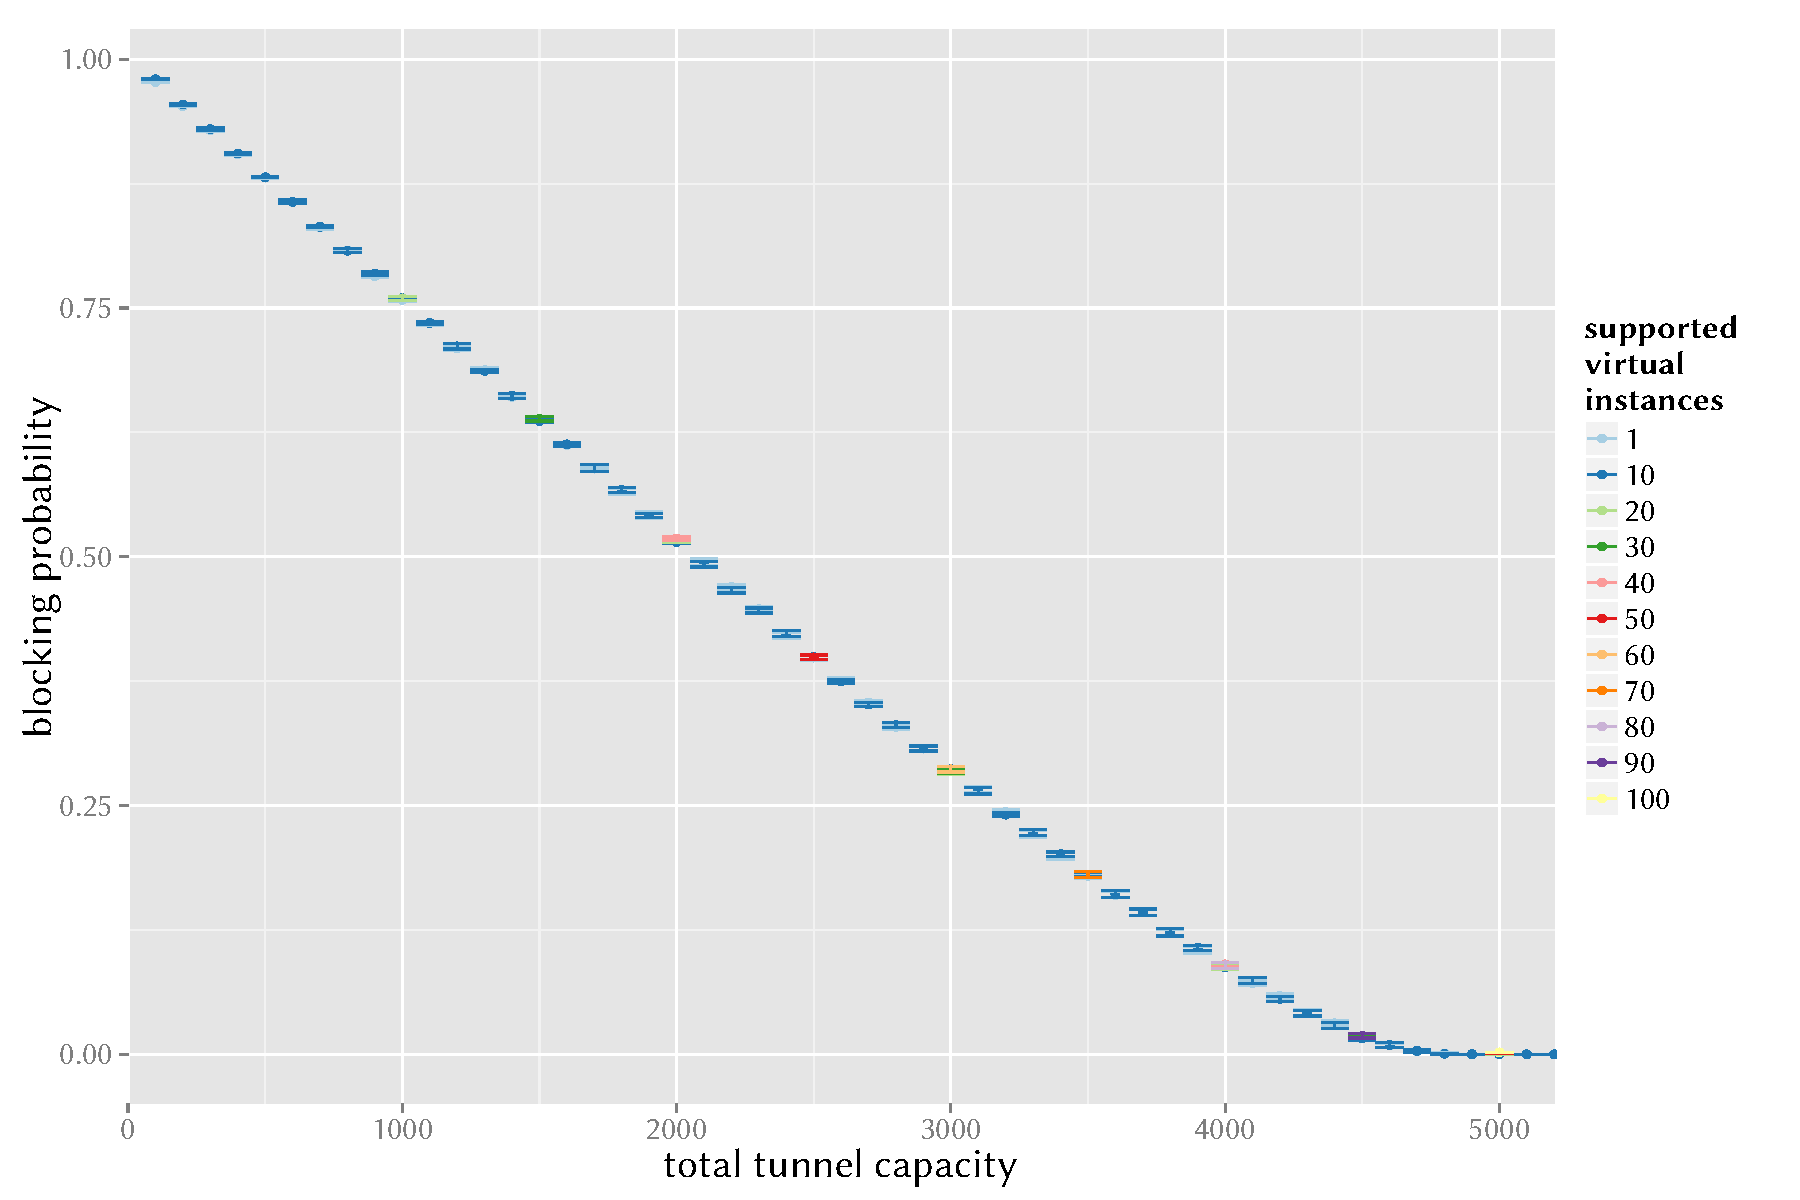
\includegraphics[height=4.5cm]{../../chapters/041-mobilenetsmeasuring/images/R-virtualized-blocking.pdf}
	\end{center}}

\end{frame}

% \begin{frame}
% 	\frametitle{Blocking Probability}

% 	\begin{center}
% 		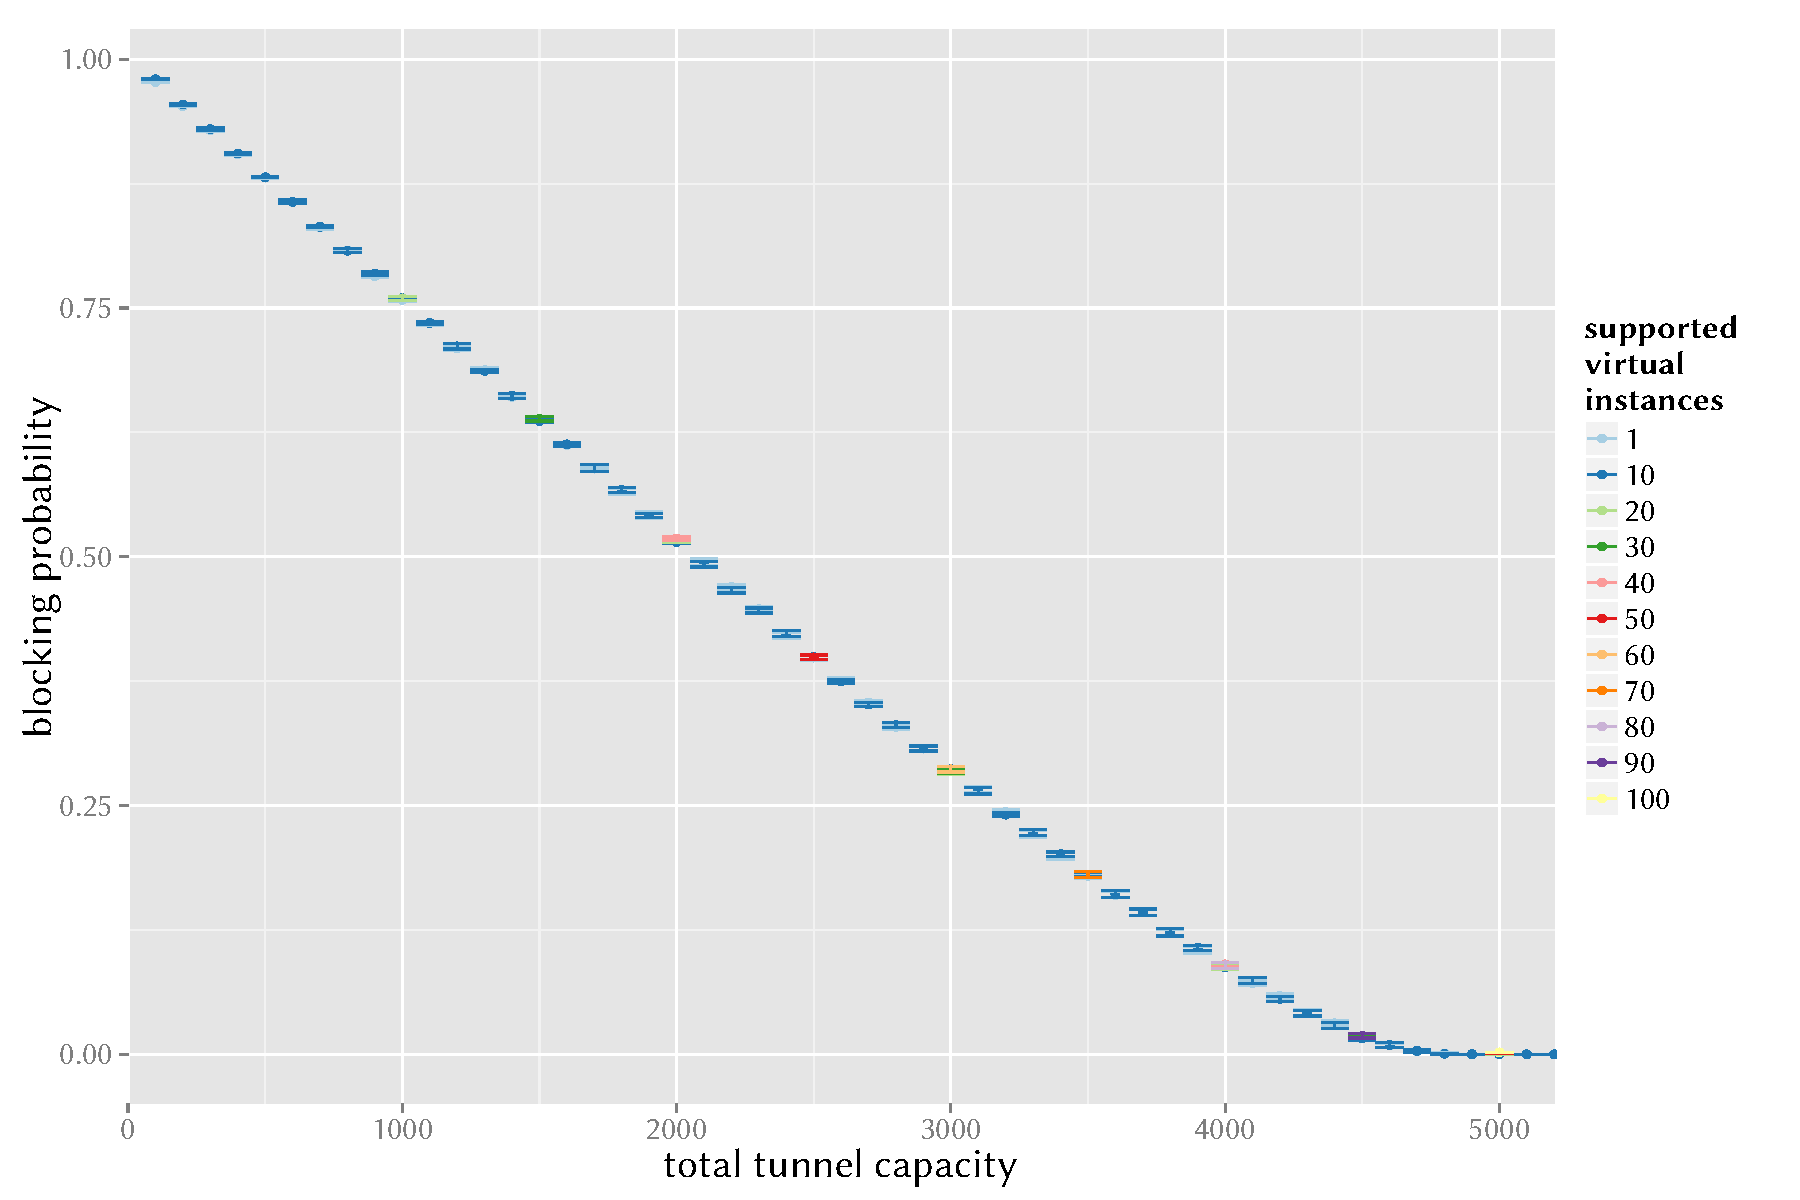
\includegraphics[height=5.5cm]{../../chapters/041-mobilenetsmeasuring/images/R-virtualized-blocking.pdf}
% 	\end{center}

% 	\begin{itemize}
% 		\item Monolithic and virtualized GGSN scale equally with supported tunnels
% 		\item Negligible to no impact on $p_B$ if virtualized model is scaled by tuning $s_{max}$ instead of $m$
% 	\end{itemize}
% \end{frame}




\begin{frame}
	\frametitle{Virtualized GGSN Resource Usage}

	\begin{center}
		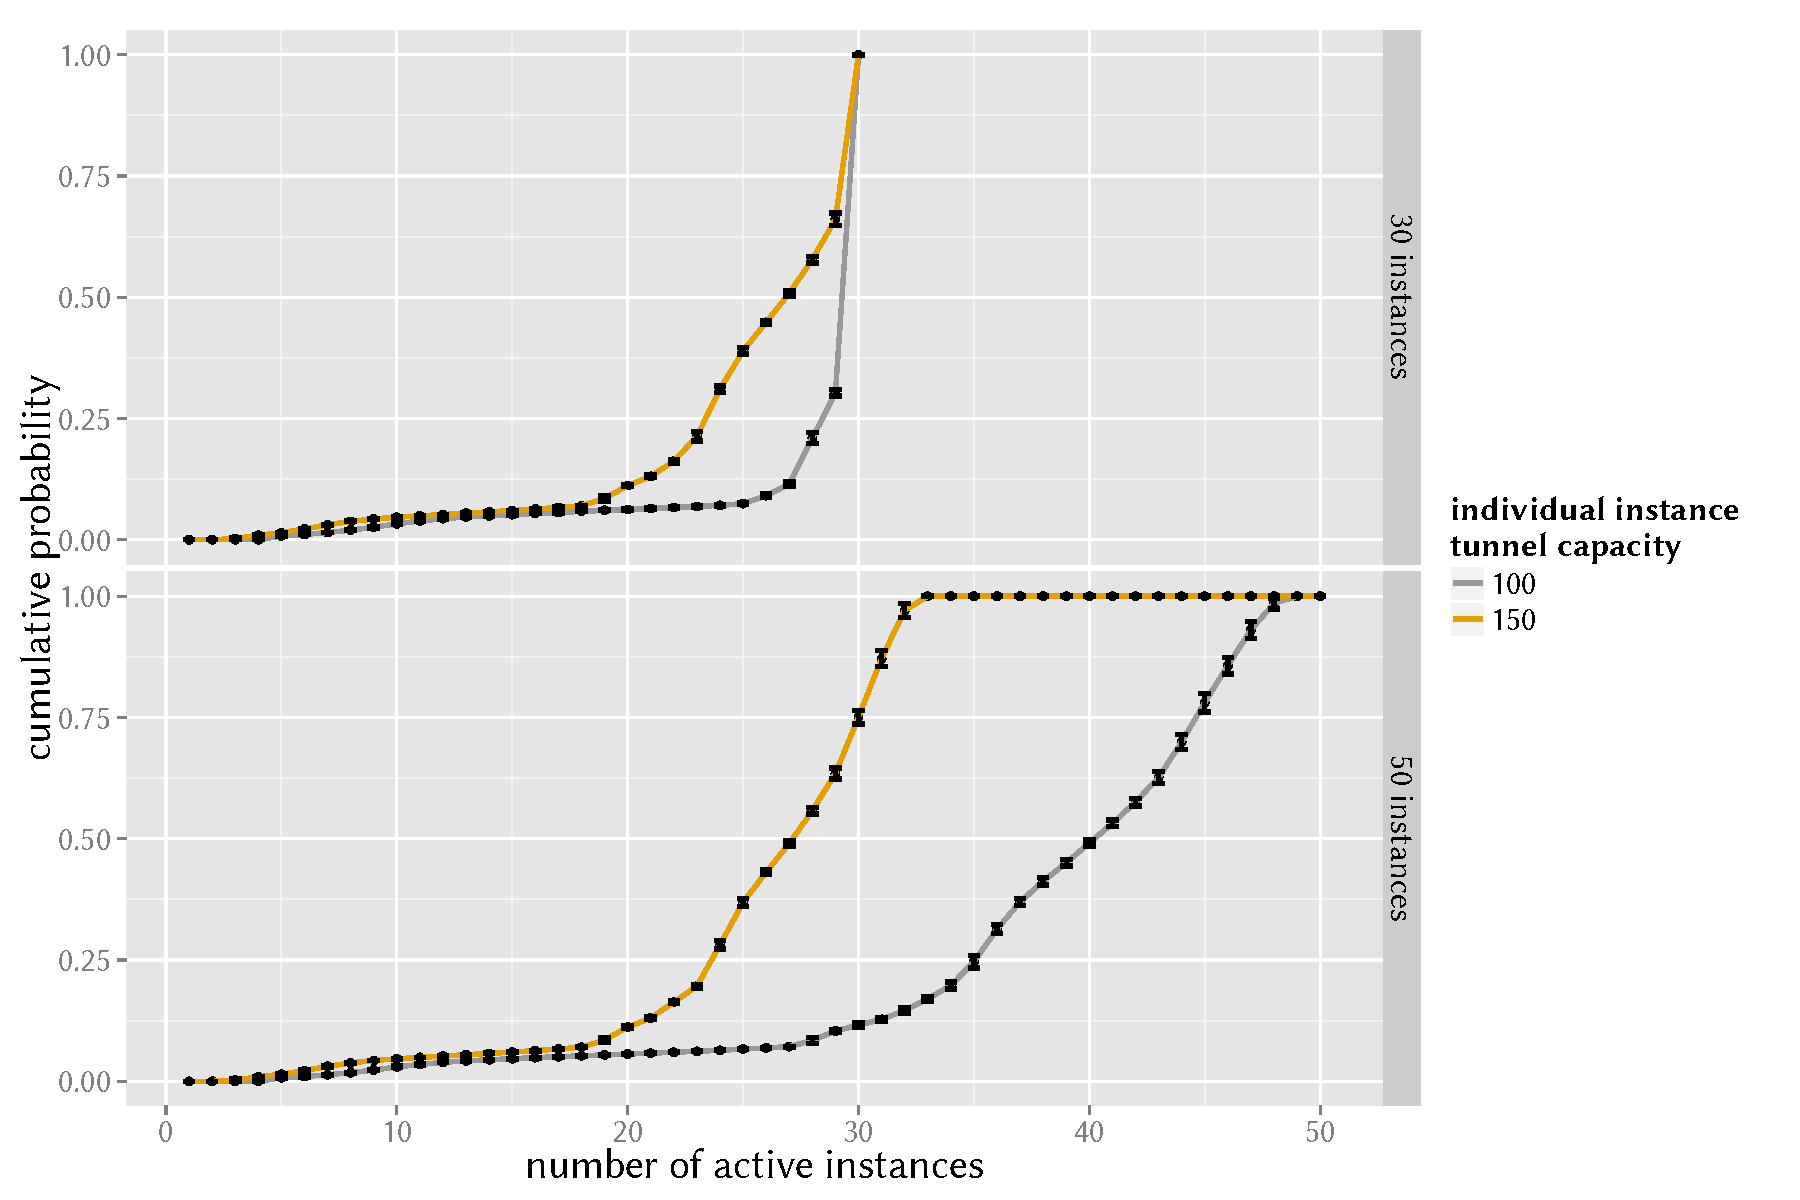
\includegraphics[height=5cm]{../../chapters/041-mobilenetsmeasuring/images/R-virtualized-instanceuse.pdf}
	\end{center}

	\begin{itemize}
		\item Monolithic and virtualized GGSN scale equally with supported tunnels
		\item Scaling VM model by VM count instead of size has minimal impact on $p_B$
		%\item System scales both up (tunnels/instance) and out (instances)
		\item Unused instances can be shut down for increased energy efficiency compared to monolithic model
	\end{itemize}
\end{frame}





%%%%%%%%%%%%%%%%%%%%%%%%%%%%%%%%%%%%%%%%%%%%%%%%%%%%%%%%%%%%%%%%%%%%%%%%%%%%%%%%
\section{Modeling Reliable Streaming}
%%%

\begin{frame}
	\frametitle{Introduction}
\end{frame}


\begin{frame}
	\frametitle{Streaming Categorization}
\end{frame}


\begin{frame}
	\frametitle{Reliable Streaming}

	Pure Progressive
	Segmented
	Adaptive

	Stalling as sole quality metric
\end{frame}



\begin{frame}
	\frametitle{Playback and Retrieval Strategies}

	Pure Progressive
	Segmented
	Adaptive
	\begin{figure}

	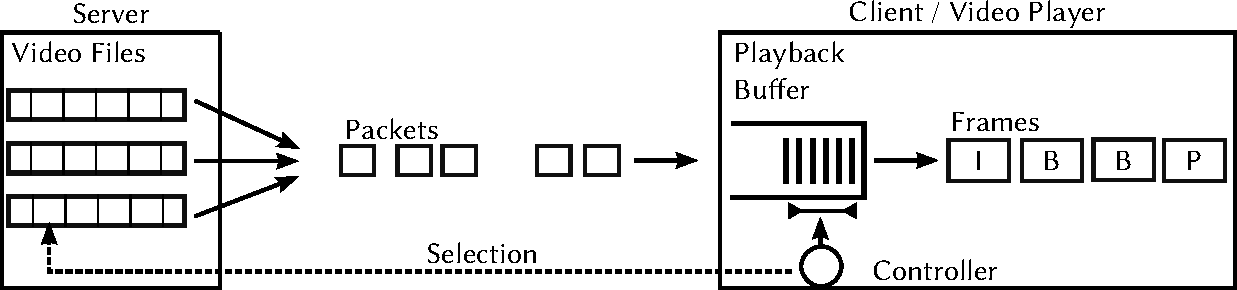
\includegraphics[height=2cm]{../../chapters/03-streaming/images/playback-model.pdf}
	\caption{Reliable streaming playback model based on buffer control.}
	\end{figure}

\end{frame}

\begin{frame}
	\frametitle{Playback Strategies Parameter Space}
	\begin{columns}[T]
		\column{0.5\textwidth}
		\begin{figure}
			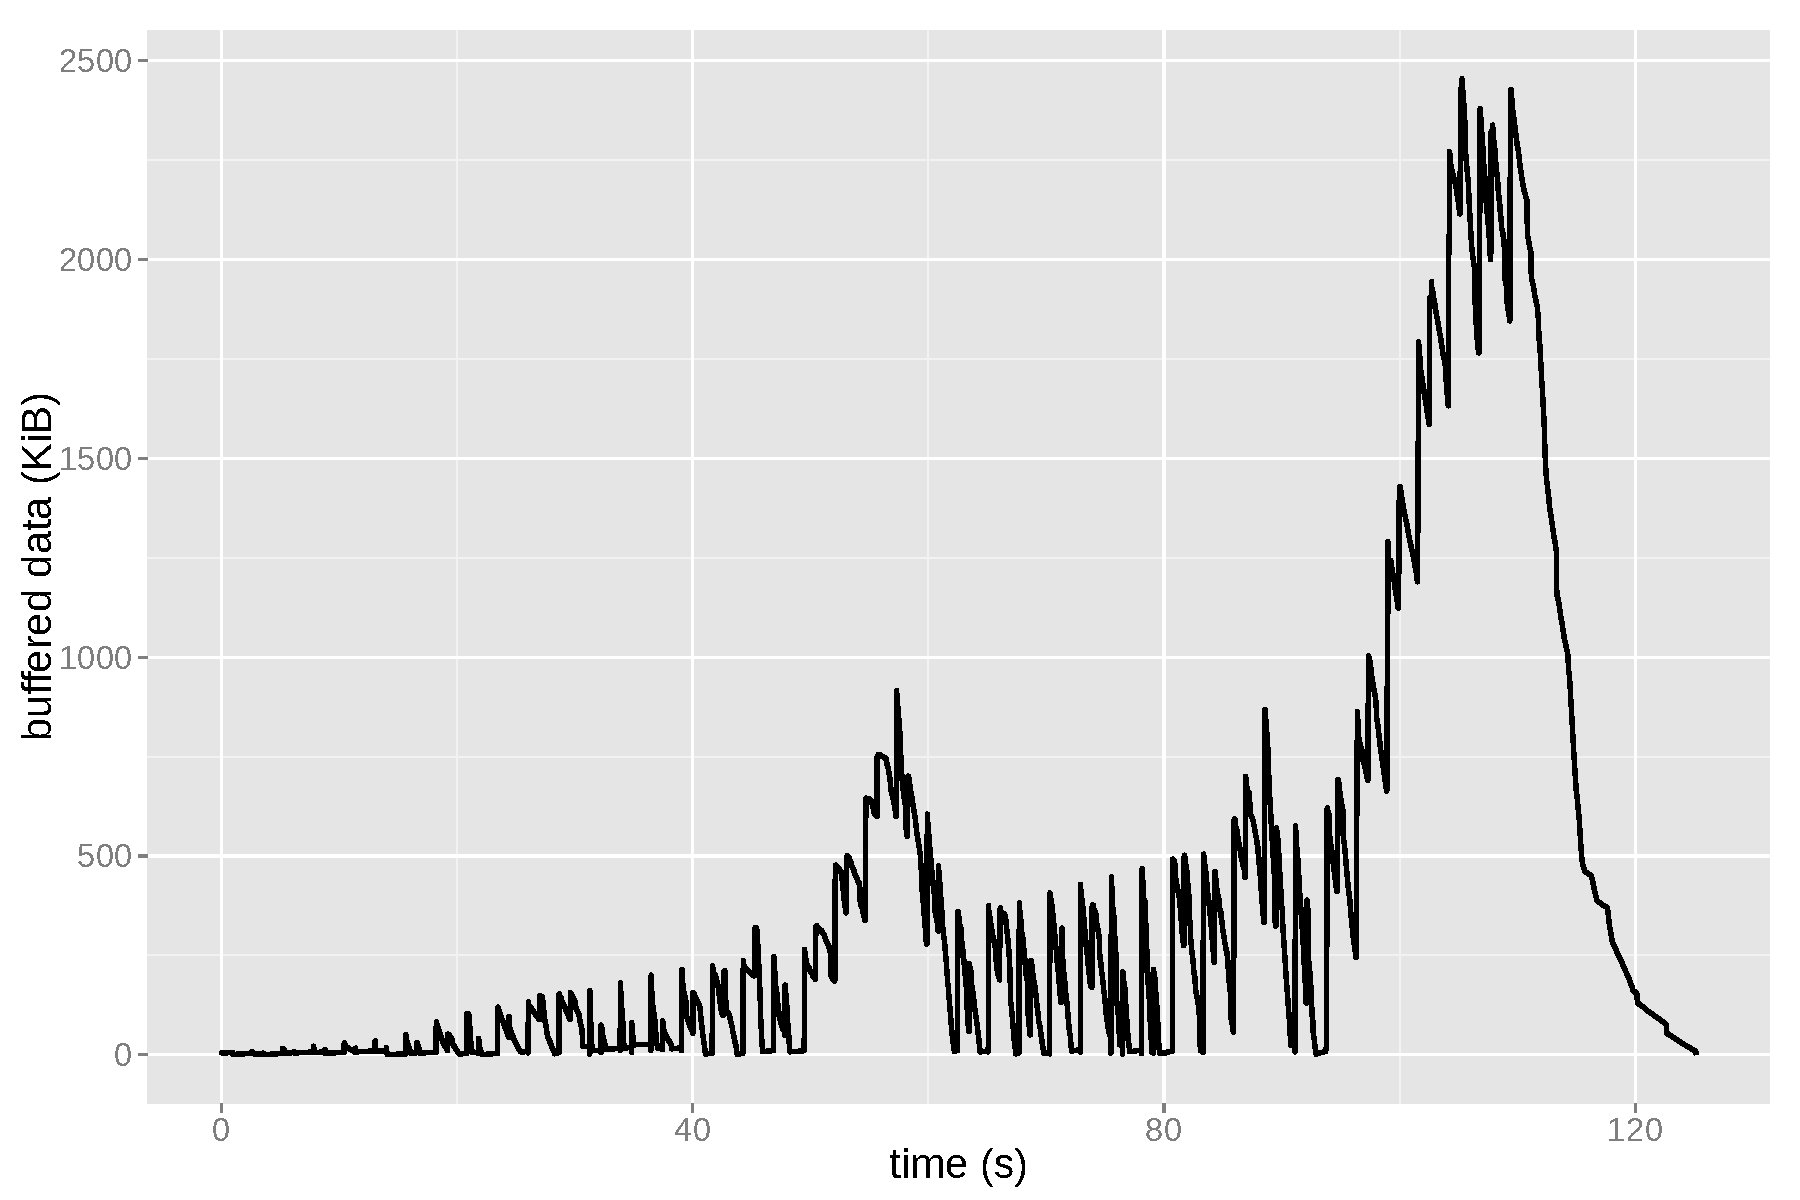
\includegraphics[width=1.0\columnwidth]{../../chapters/03-streaming/images/R-bufferlevel-stall.pdf}
			\caption{Buffer fill level with null strategy; \SI{33}{\second} total stalling.}
		\end{figure}

		\column{0.5\textwidth}
		\begin{figure}
			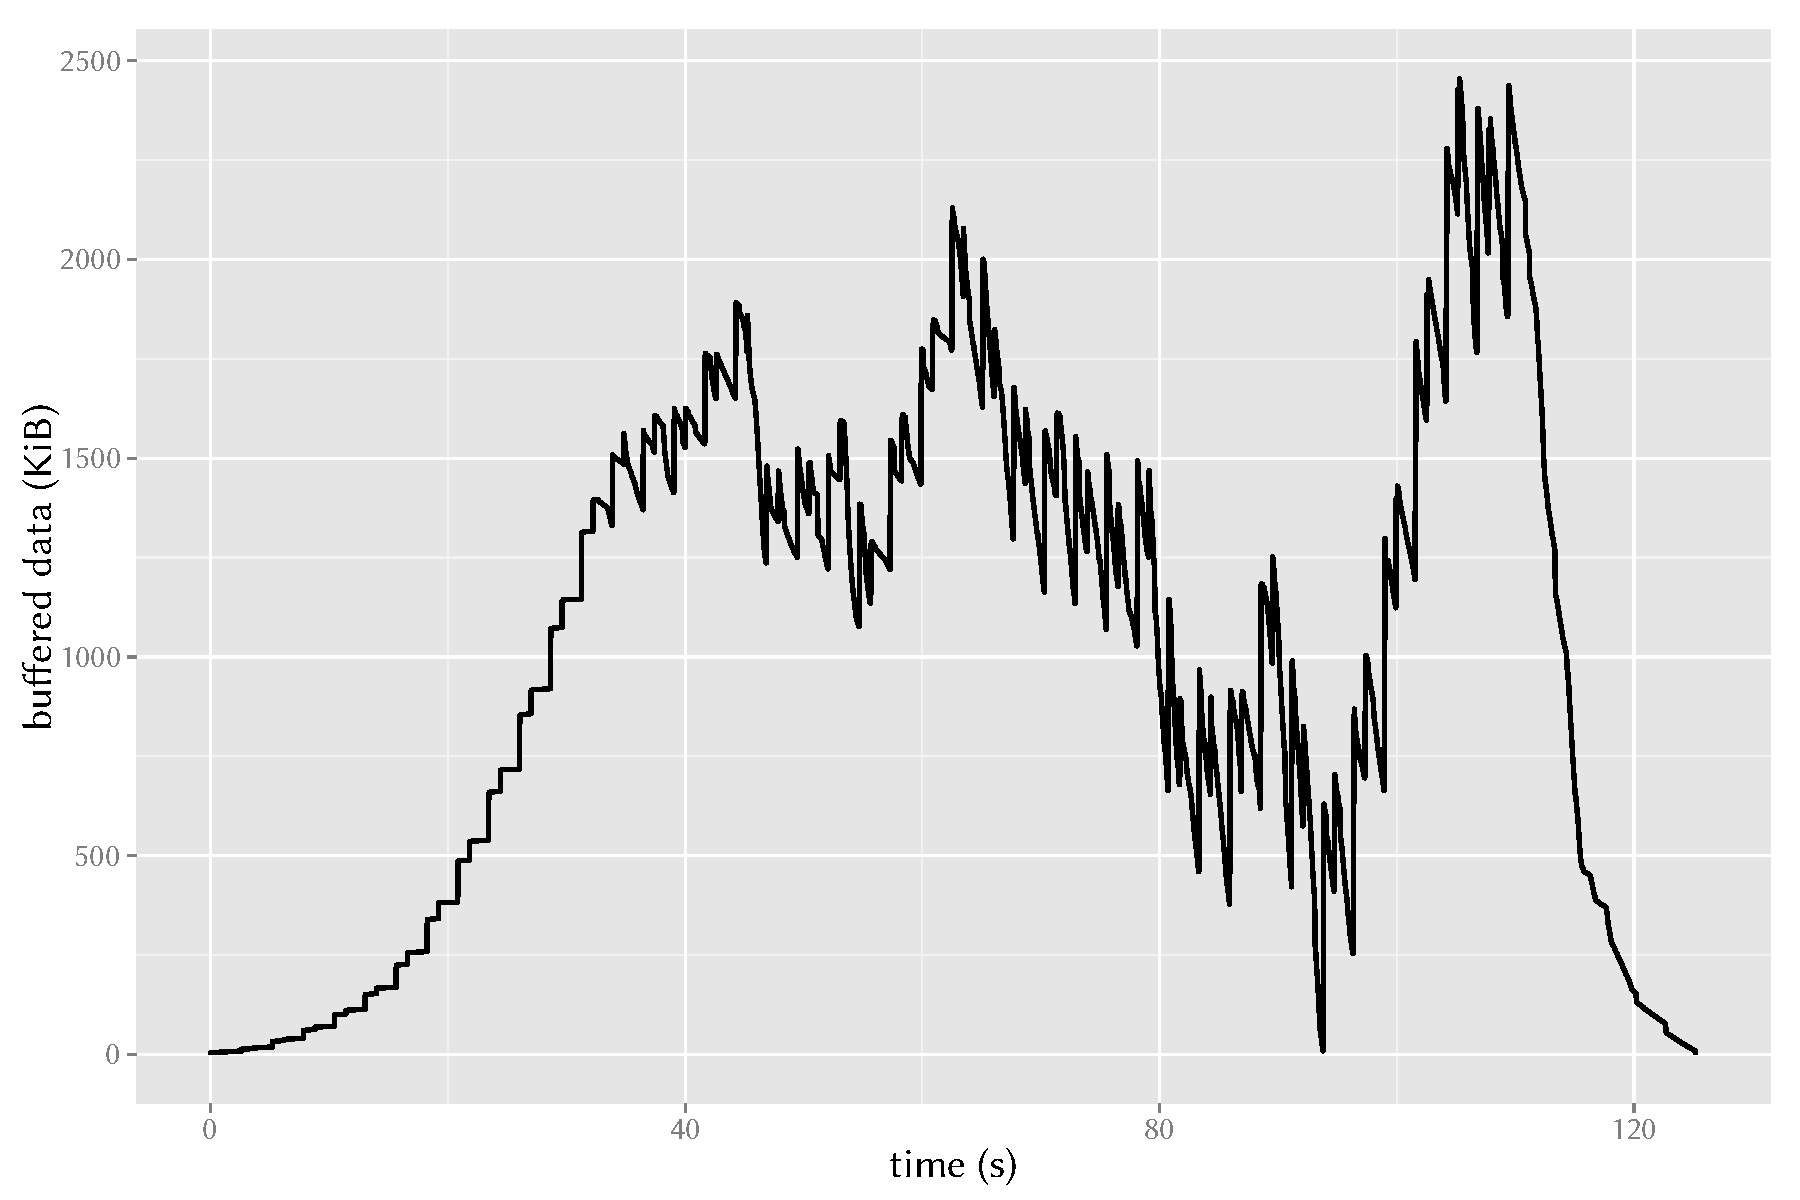
\includegraphics[width=1.0\columnwidth]{../../chapters/03-streaming/images/R-bufferlevel-startdelay.pdf}
			\caption{Sample Buffer fill level for the delayed playback predictive strategy, \SI{33}{\second} total stalling.}
		\end{figure}
	\end{columns}
\end{frame}


\begin{frame}
	\frametitle{Streaming Measurements}

	\begin{figure}
		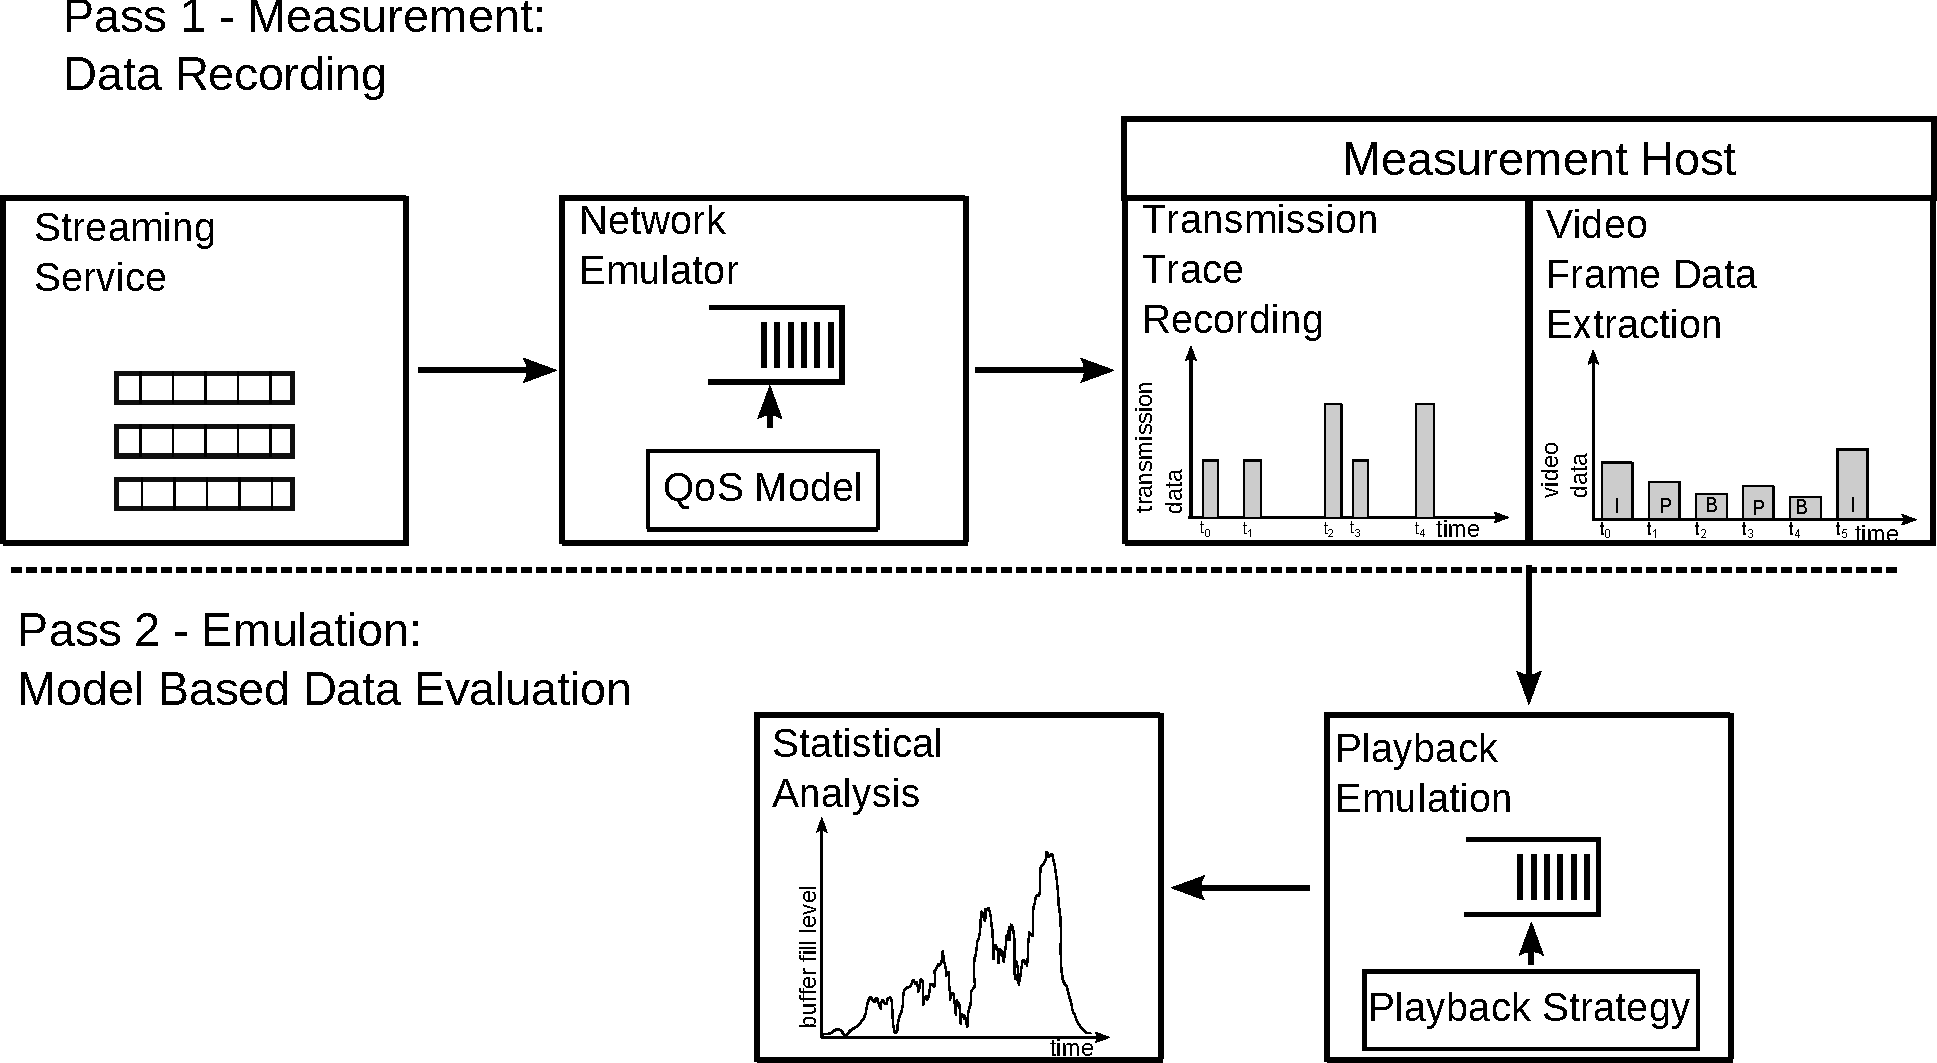
\includegraphics[height=4cm]{../../chapters/03-streaming/images/measurement-model.pdf}
		\caption{Measurement framework for progressive streaming playback strategies.}
	\end{figure}

	Buffer model:
	\begin{equation*}
		\mathit{buffer}(t) = \sum_{0}^{t} \text{data}_\mathrm{received} - \sum_{0}^{t} \text{data}_\mathrm{played}
	\end{equation*}

	Measure stall duration and number of occurrences



\end{frame}



\begin{frame}
	\frametitle{Streaming Measurements: Latency}

	\begin{figure}
		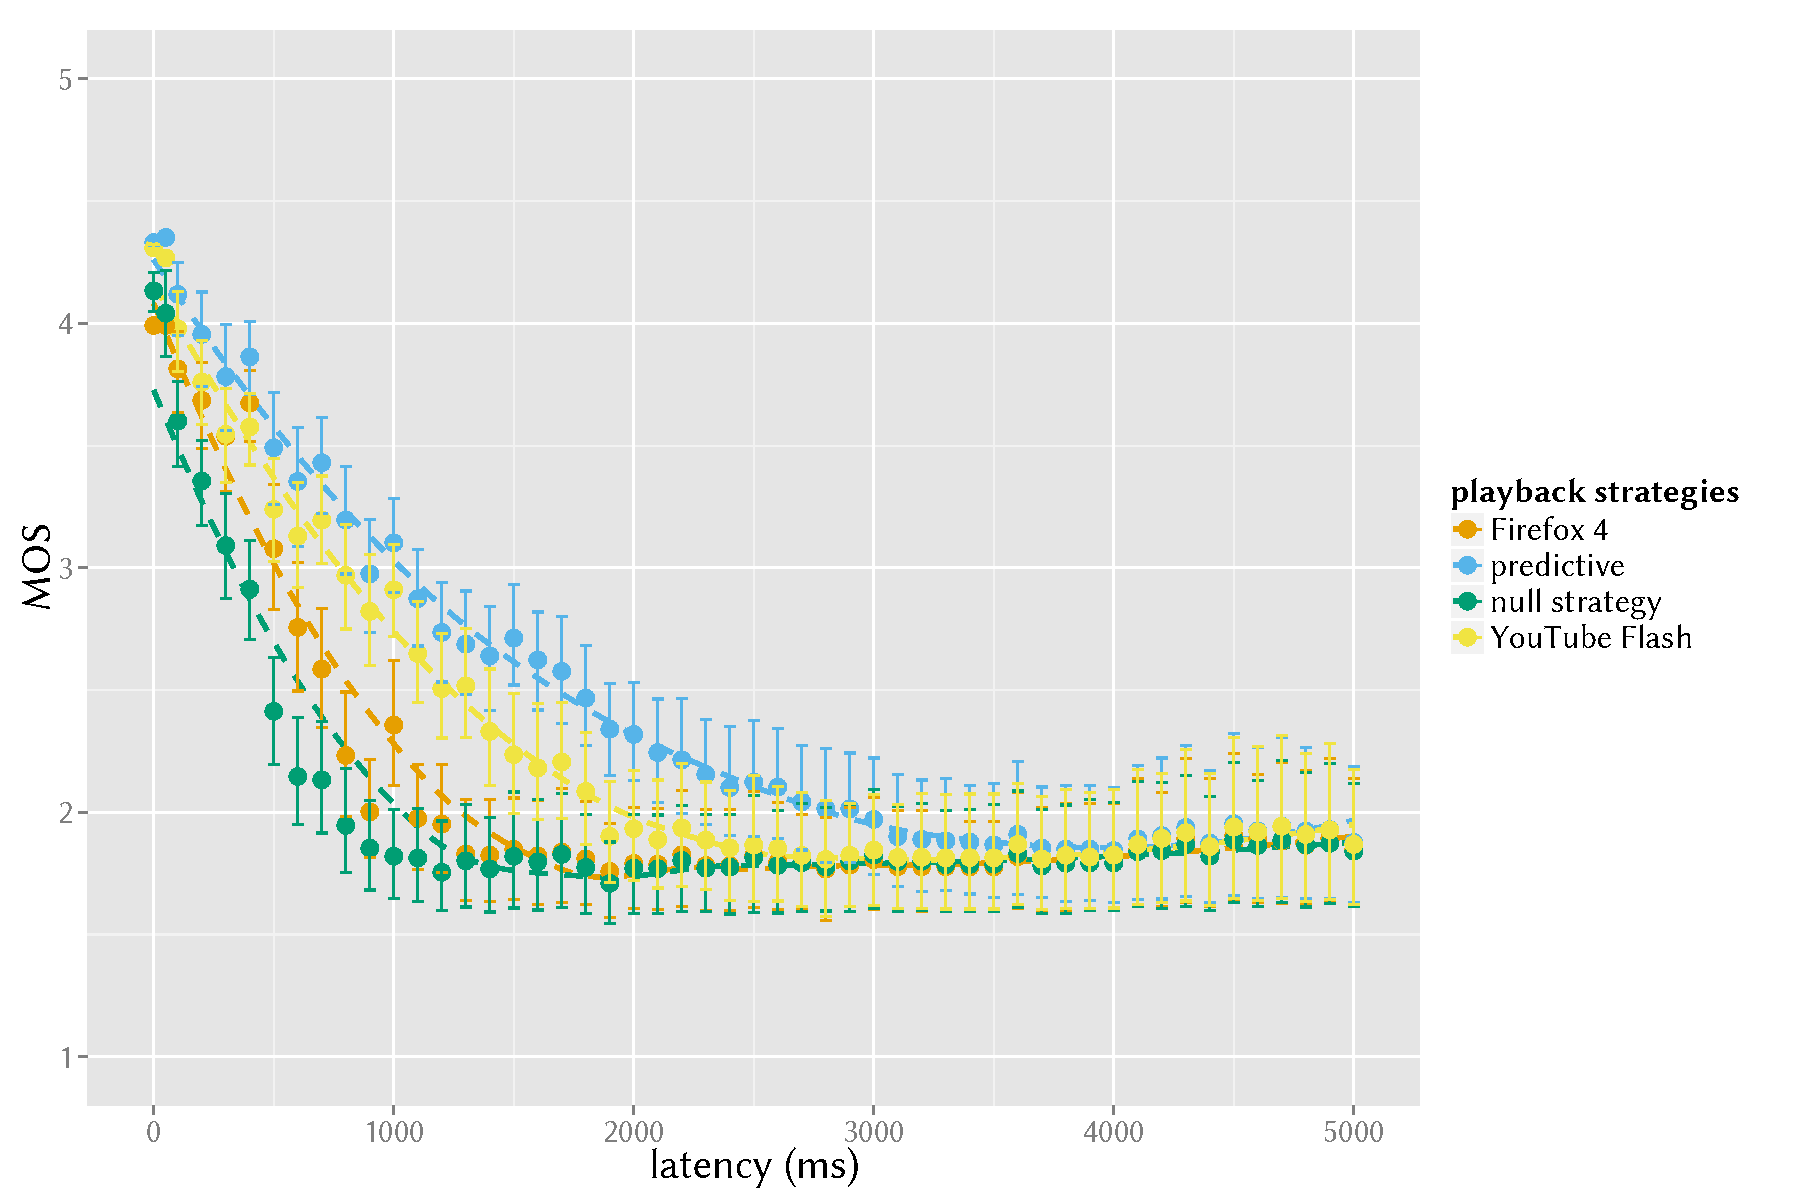
\includegraphics[height=4cm]{../../chapters/03-streaming/images/R-playbackemulation-qoe-latency.pdf}
		\caption{Calculated MOS for the latency measurement series.}
	\end{figure}
	Facilitated QoE equation \cite{hossfeld2013youtubeqoe}
	\begin{equation*}
		\phantom{.} f(L,N) = 3.50e^{-(0.15L +0.19)N} + 1.50 \text{ for } L \in \mathbb{R}^{+}, N \in \mathbb{N}.
	\end{equation*}

\end{frame}


%%%%%%%%%%%%%%%%%%%%%%%%%%%%%%%%%%%%%%%%%%%%%%%%%%%%%%%%%%%%%%%%%%%%%%%%%%%%%%%%
\section{Reliable Streaming in Mobile Networks}
\subsection{Influences on Streaming Approaches}
%%%

\begin{frame}
	\frametitle{Introduction}
\end{frame}

\begin{frame}
	\frametitle{Layer Influences}

	Time scales of layer operation

	constantly changing protocol details/implementations with often unforeseen effects on specific applications (e.g. streaming)
	example with most number of changes: TCP in Linux kernel (show table?)
\end{frame}



%%%%
\subsection{Cross-Layer Improvement Model}
%%%%


\begin{frame}
	\frametitle{Cross-Layer Information Exchange Model}

	\begin{figure}
		\centering
		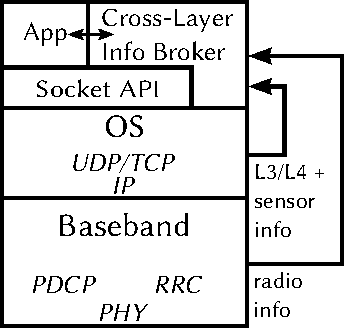
\includegraphics[height=3cm]{../../chapters/05-mobilestreaming/images/cross-layer-model.pdf}
		\caption{Model and architecture of the proposed cross-layer information exchange.}
	\end{figure}
\end{frame}

\begin{frame}
	\frametitle{Cross-Layer Streaming Benefits}

	\begin{columns}[T]
		\column{0.5\textwidth}
		\begin{figure}
			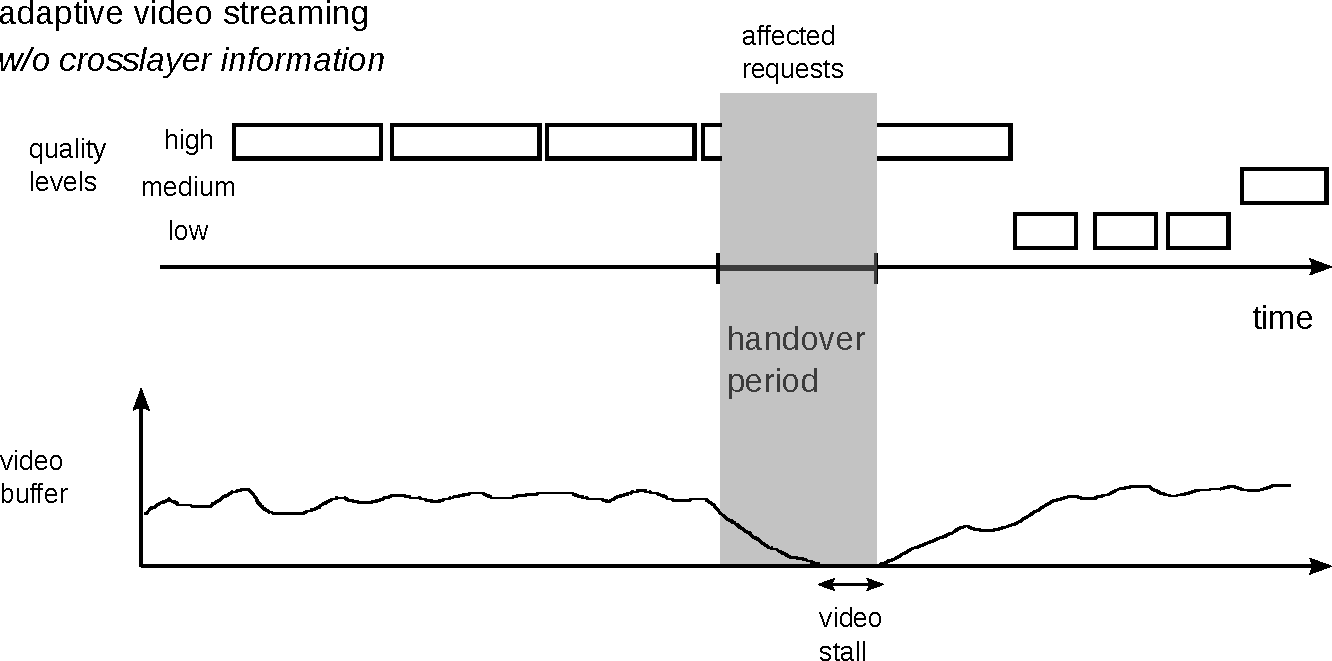
\includegraphics[width=\columnwidth]{../../chapters/05-mobilestreaming/images/adaptive-streaming-no-cl.pdf}
			\caption{Stalling occurs without handover hinting.}
		\end{figure}

		\column{0.5\textwidth}
		\begin{figure}
			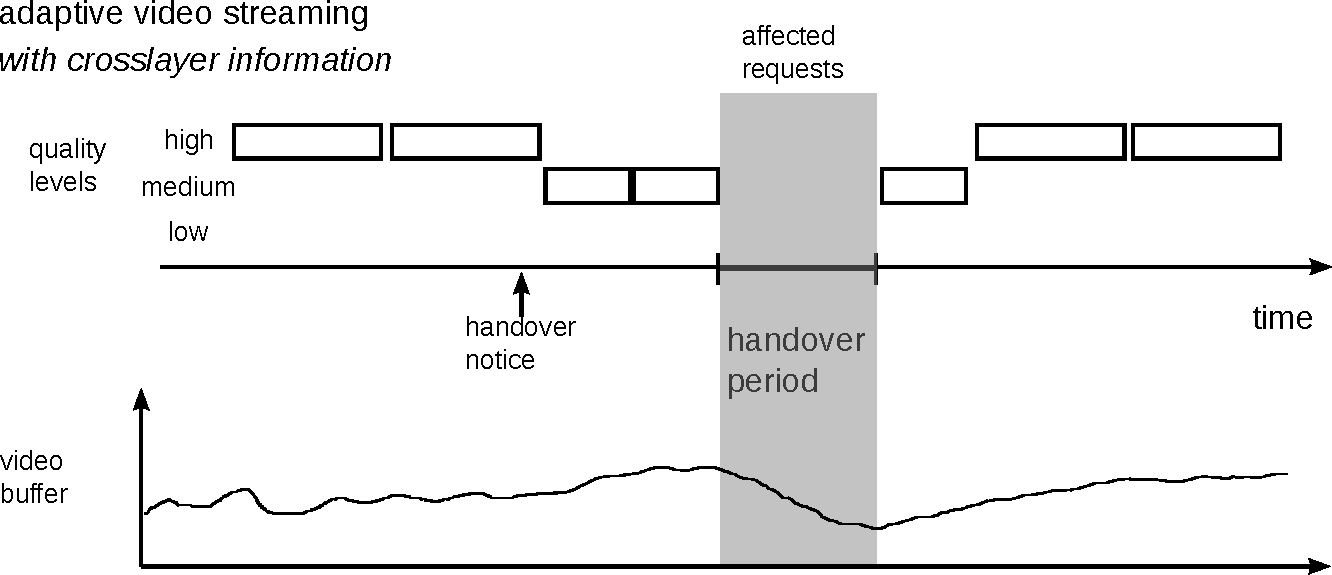
\includegraphics[width=\columnwidth]{../../chapters/05-mobilestreaming/images/adaptive-streaming-cl.pdf}
			\caption{Stalling can be prevented by hinting and proactively filling the playback buffer.}
		\end{figure}
	\end{columns}
\end{frame}



%%%%%%%%%%%%%%%%%%%%%%%%%%%%%%%%%%%%%%%%%%%%%%%%%%%%%%%%%%%%%%%%%%%%%%%%%%%%%%%%
\subsection{Measuring Mobile Reliable Streaming}
%%%

\begin{frame}
	\frametitle{Introduction}
\end{frame}


\begin{frame}
	\frametitle{Active Measurements}

Instead of passive core traces
\end{frame}

\begin{frame}
	\frametitle{Sensorium 1}
	Importance of additional metadata in active mobile measurements
	privacy issues!
	let the user control data granularity
\end{frame}


\begin{frame}
	\frametitle{Sensorium 2}

	\begin{figure}
		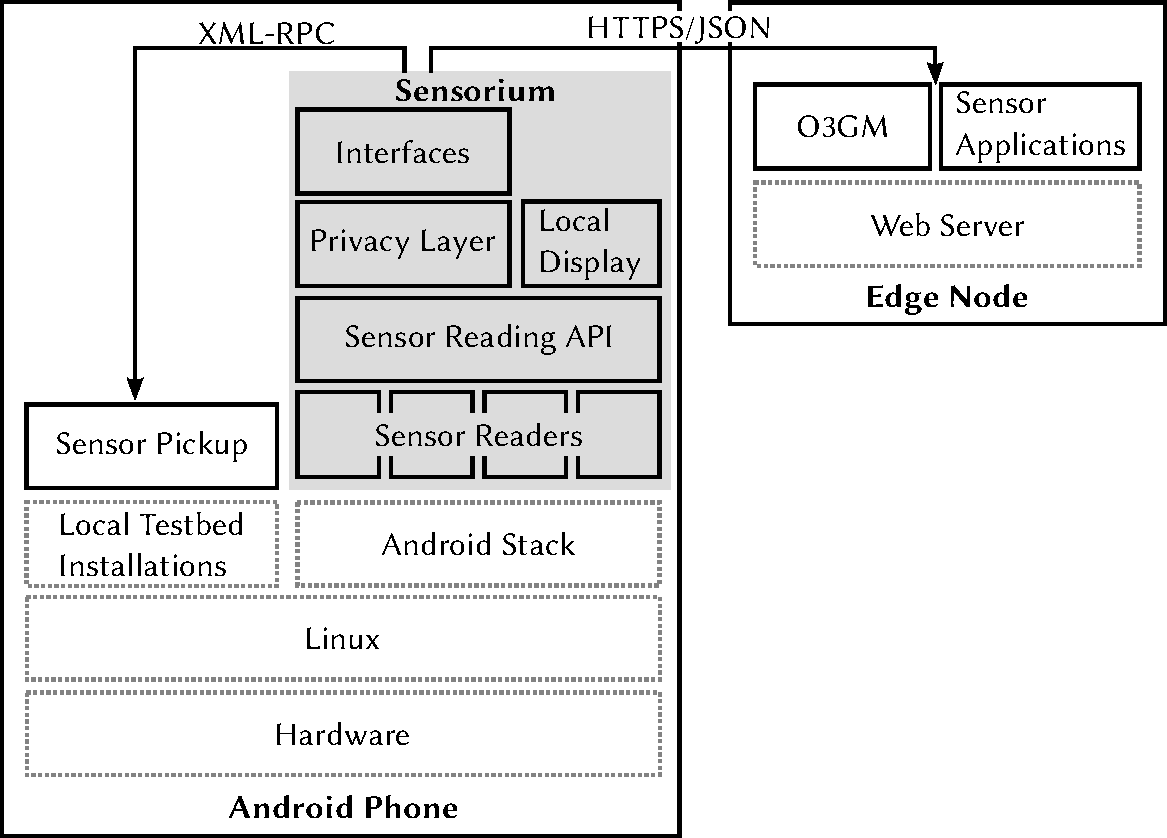
\includegraphics[height=5cm]{../../chapters/06-mobilestreamingmeasurements/images/sensorium-arch.pdf}
		\caption{Sensorium architecture interfacing with other applications. Previously existing components are marked with a dotted line.}
	\end{figure}

\end{frame}


\begin{frame}
	\frametitle{Mobile Streaming Simulation}

	Effort to find a suitable mobile streaming simulator: hard!

	No complete, up-to-date UMTS simulator

	Only radio interface simulated, not enough for a network-wide view

	Even then, only just user-path through the network, no control plane

	Questionable viability of every mobile simulation framework

	Reason: Sheer volume and complexity of control plane (tens of thousands of spec pages)
\end{frame}


\begin{frame}
	\frametitle{Mobile Streaming Simulation}

	Restrict to user plane and choose ns-3 with Lena (LTE Framework)

	Has a usable tcp/ip stack (still completely different to actual implementations)

	Can facilitate NSC (network simulation cradle), but mostly very old actual stacks

	Can act as network emulator and bridge in/out actual traffic (must operate in real-time, performance is an issue)
\end{frame}


\begin{frame}
	\frametitle{Mobile Streaming Simulation}

	\begin{figure}
		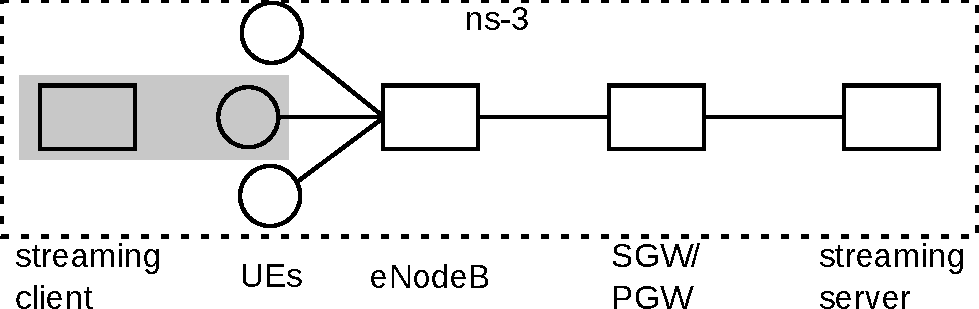
\includegraphics[height=2cm]{../../chapters/06-mobilestreamingmeasurements/images/streaming-simulation.pdf}
		\caption{LTE reliable streaming simulation testbed.}
	\end{figure}
\end{frame}


\begin{frame}
	\frametitle{Streaming Strategies}
	\framesubtitle{Four Threshold Segmented Streaming Strategy}

	\begin{figure}
		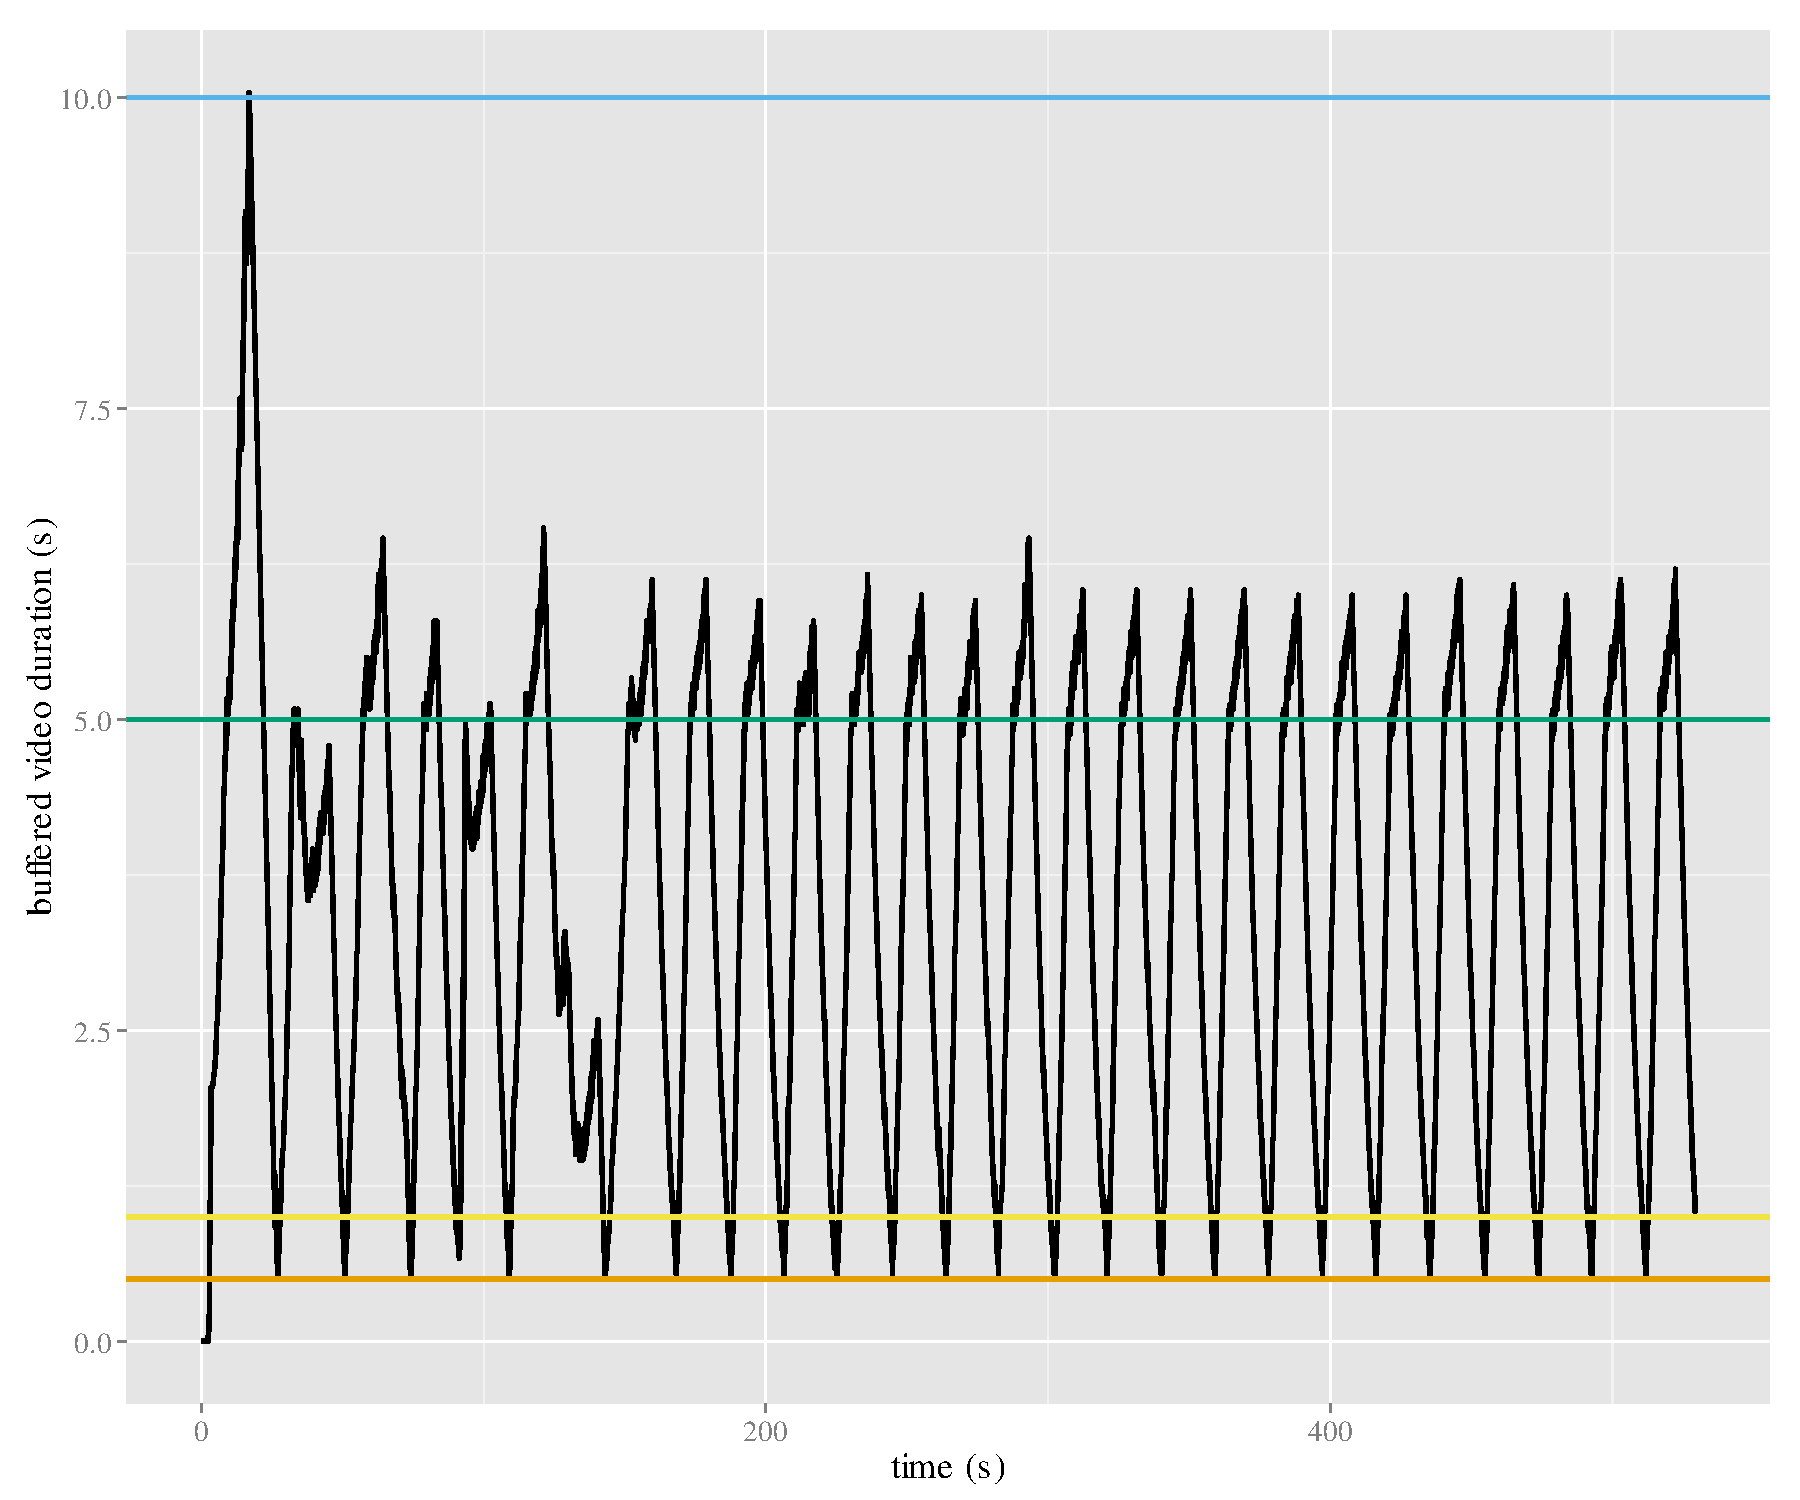
\includegraphics[height=5cm]{../../chapters/06-mobilestreamingmeasurements/images/R-ltesim-plotbuffer-time.pdf}
		\caption{Sample simulation run demonstrating the four threshold strategy.}
	\end{figure}

	Also: Six Threshold Window Scaling Adaptive Streaming Strategy

\end{frame}

\begin{frame}
	\frametitle{Simulation Evaluation}

	Scenario 1: Internet link latency and limited bandwidth

	Measure num/length of stalls, calculate Hoßfeld-QoE

	\begin{figure}
	\centering
	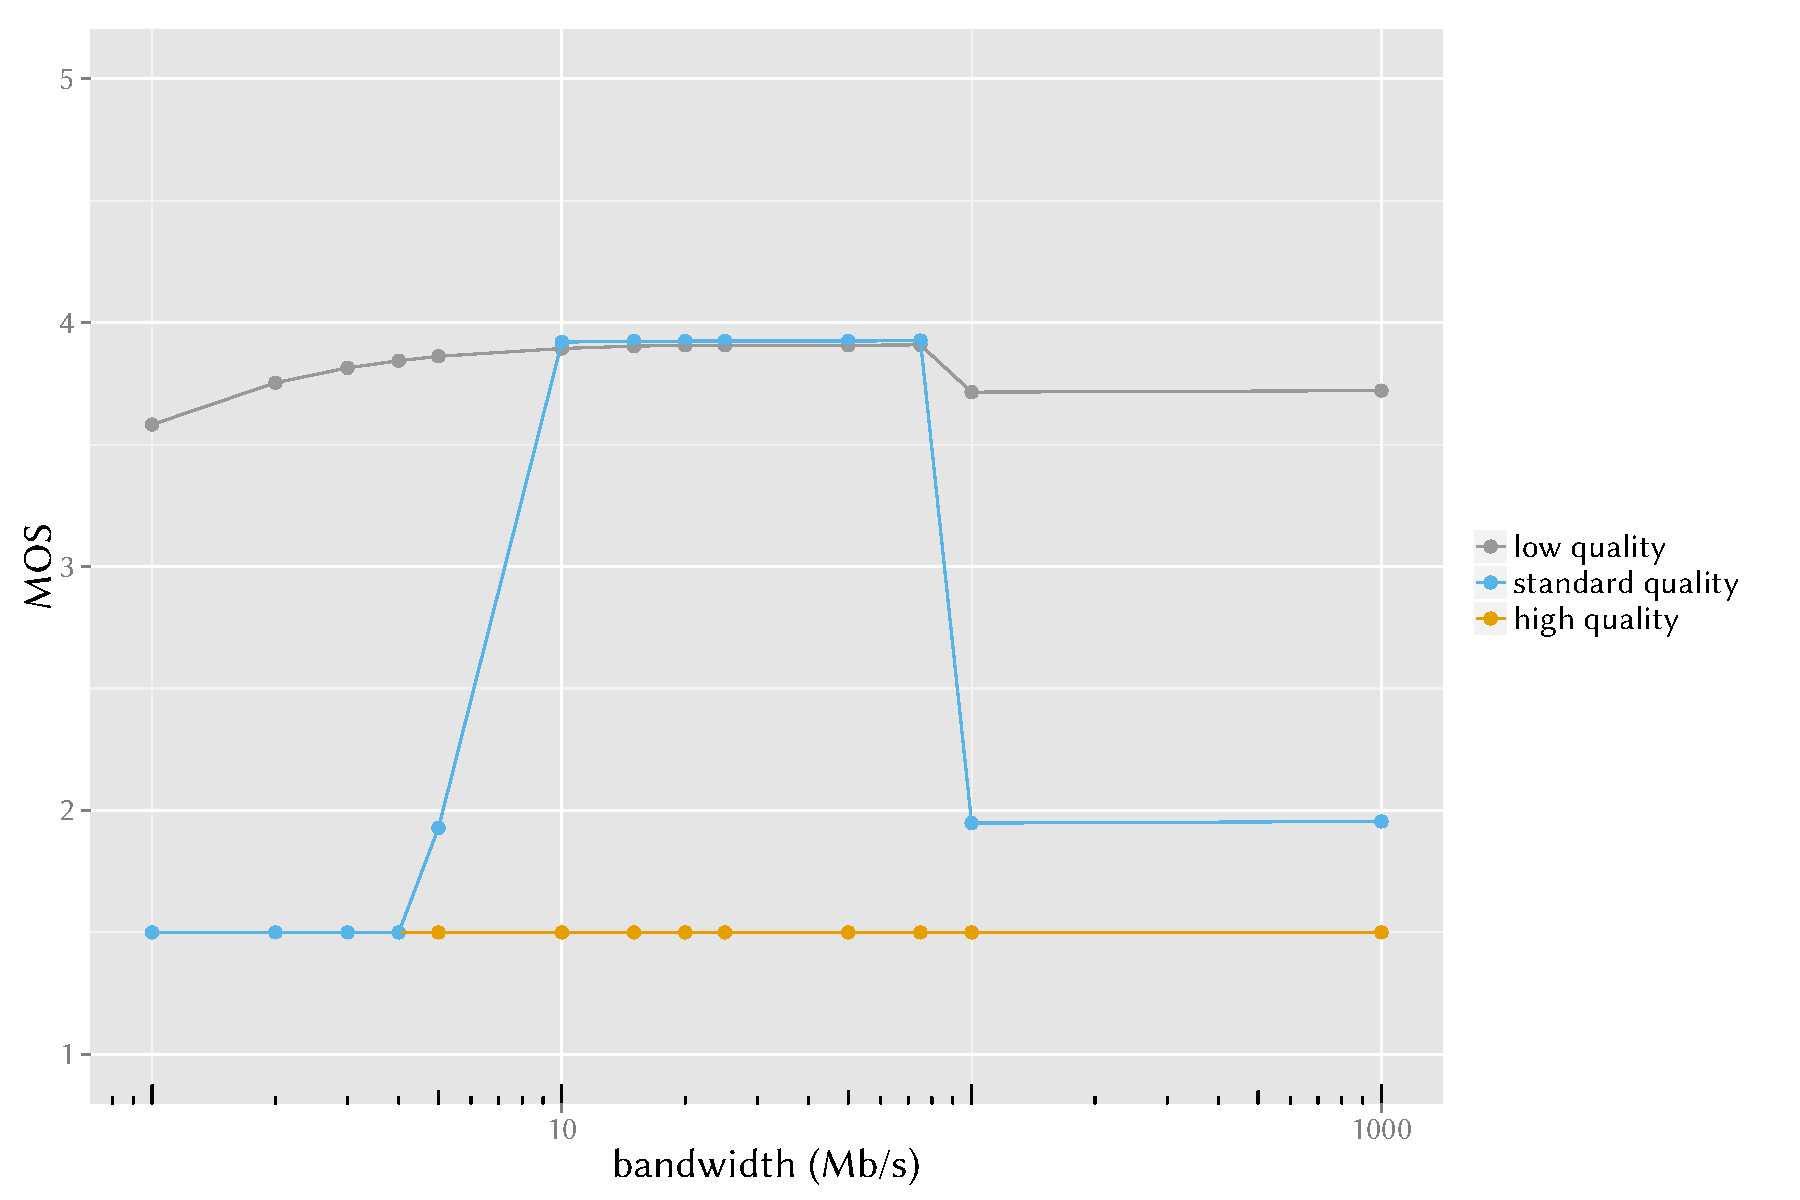
\includegraphics[height=5cm]{../../chapters/06-mobilestreamingmeasurements/images/R-ltesim-bwseries-qoe.pdf}
	\caption{Computed QoE of the reliable streaming strategy with limited bandwidth.}
	\end{figure}

\end{frame}



\begin{frame}
	\frametitle{Simulation Evaluation}
	\framesubtitle{Mobility Scenario}

	\begin{figure}
		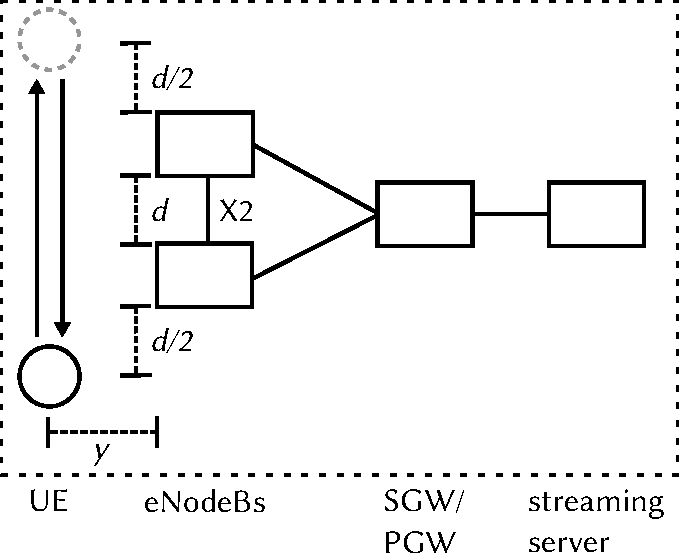
\includegraphics[height=4cm]{../../chapters/06-mobilestreamingmeasurements/images/streaming-simulation-mobility.pdf}
		\caption{Simulated handover mobility scenario using waypoints.}
	\end{figure}

\end{frame}


\begin{frame}
	\frametitle{Simulation Evaluation}
	\framesubtitle{Mobility Scenario}

	\begin{figure}
		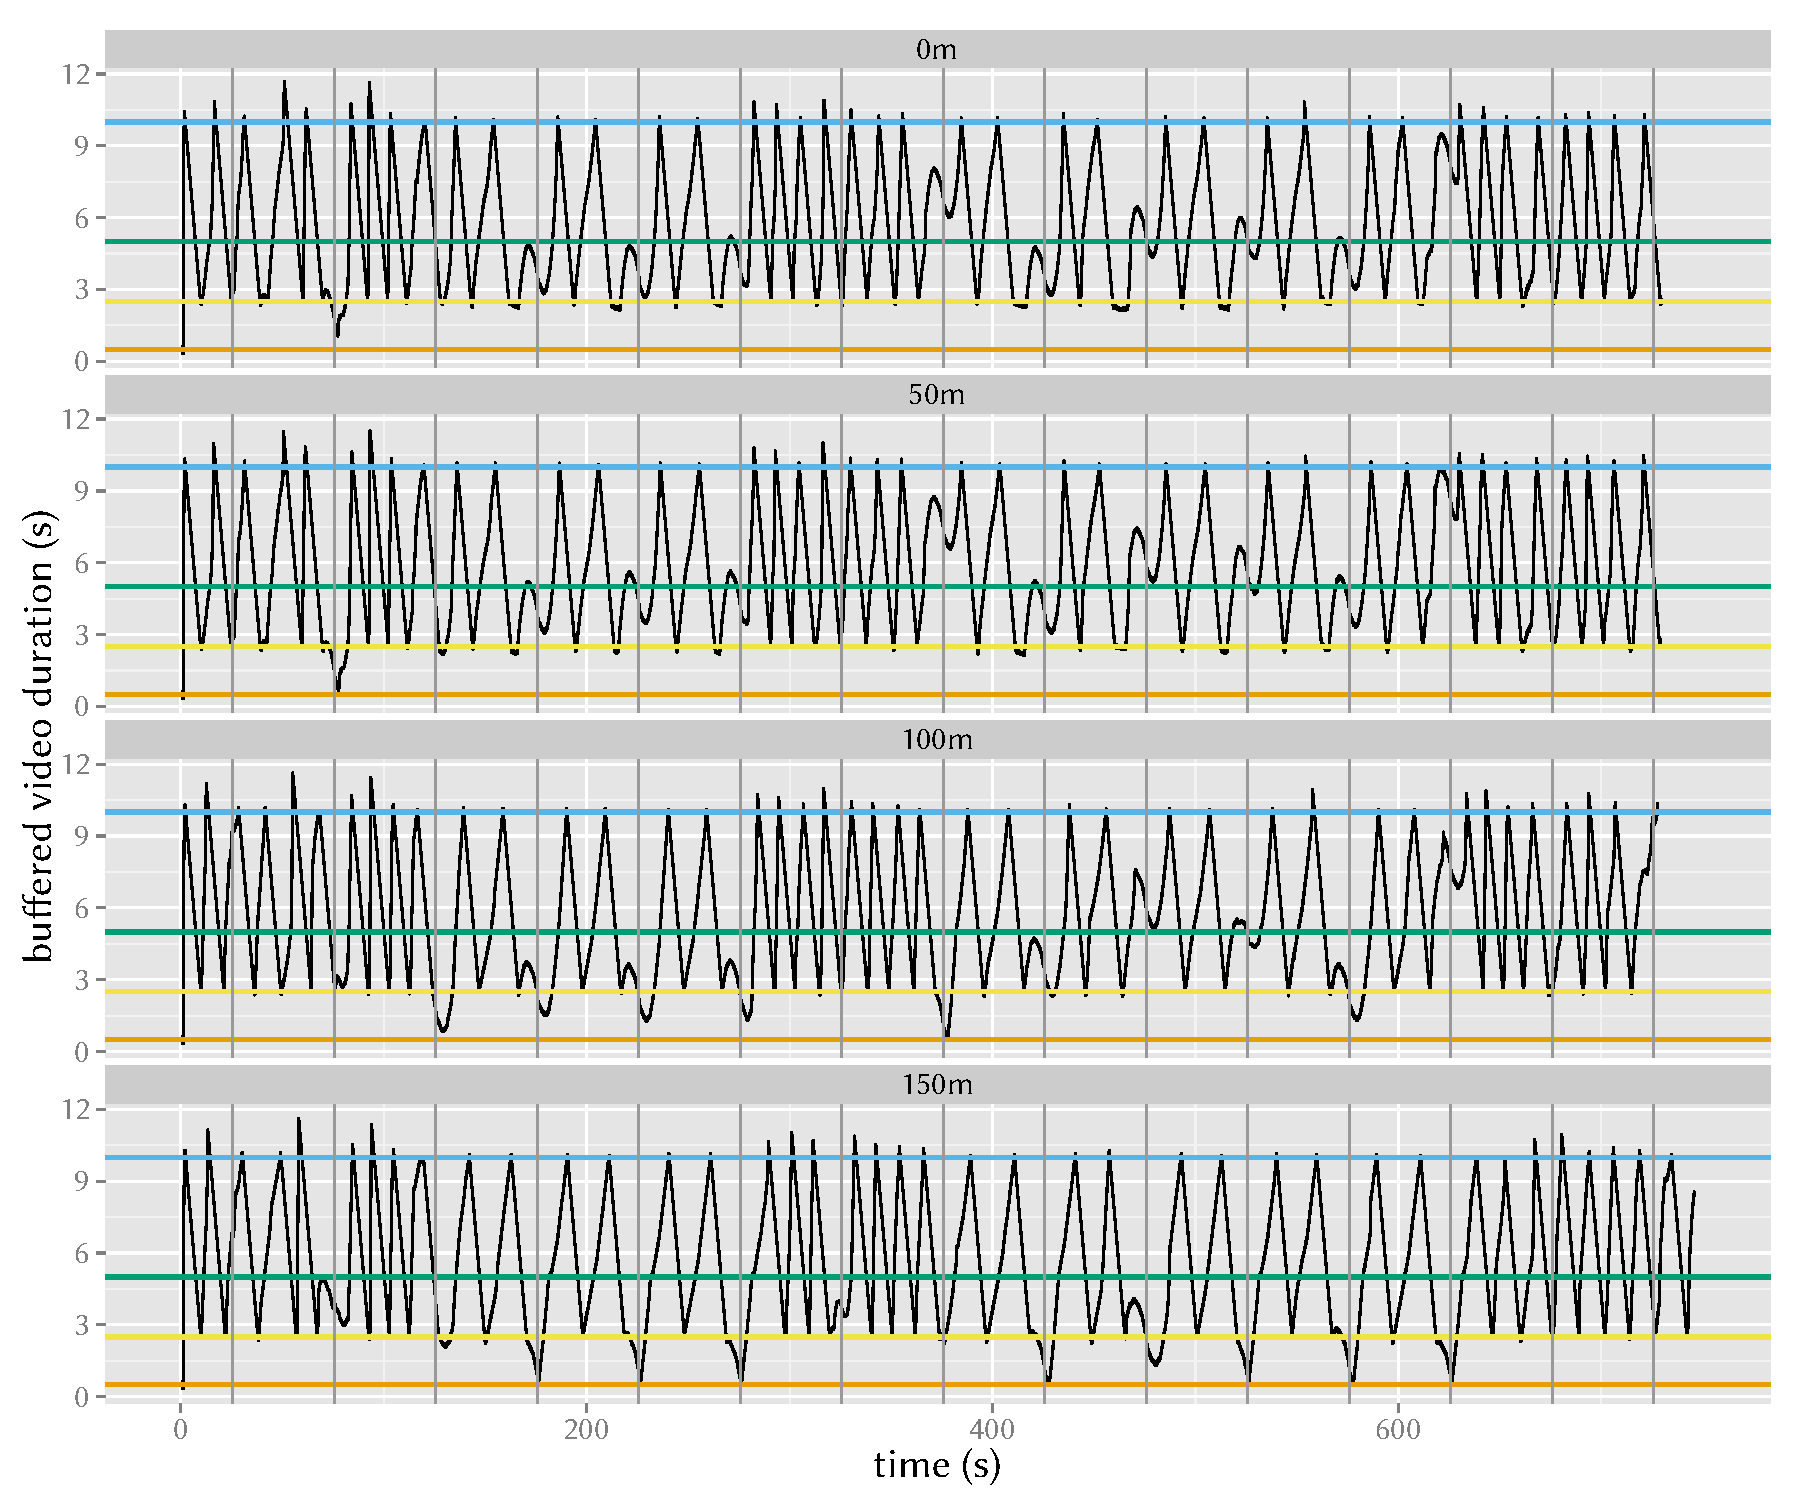
\includegraphics[height=6cm]{../../chapters/06-mobilestreamingmeasurements/images/R-ltesim-plotbuffer-mobility-facets.pdf}
		\caption{Playback buffer time series of the simulated mobility experiments with increasing distance between device and eNBs.}
	\end{figure}

\end{frame}


%%%%%%%%%%%%%%%%%%%%%%%%%%%%%%%%%%%%%%%%%%%%%%%%%%%%%%%%%%%%%%%%%%%%%%%%%%%%%%%%
\section{Conclusions}
%%%

\begin{frame}
	\frametitle{Conclusion}

	\begin{itemize}
		\item Investigated tunnel properties in core network dataset

		\begin{itemize}
			\item Non-stationary Poisson arrivals
			\item Tunnel duration with general distribution
		\end{itemize}

		\item Erlang loss models for tunnel load at a mobile core network's GGSN
		\begin{itemize}
			\item Monolithic GGSN representing today's makeup
			\item Virtualized GGSN proposal with improved scalability and efficiency
		\end{itemize}

		\item Simulative evaluation of the model

		\item Enable mobile network dimensioning based on tunnel blocking rate instead of only user traffic volume


	\end{itemize}

\end{frame}

%%%%%%%%%%%%%%%%%%%%%%%%%%%%%%%%%%%%%%%%%%%%%%%%%%%%%%%%%%%%%%%%%%%%%%%%%%%%%%%%
\section*{}
%%
\begin{frame}
	\frametitle{Thanks!}

	\centering
		\Large Questions?
\end{frame}




%%%%%%%%%%%%%%%%%%%%%%%%%%%%%%%%%%%%%%%%%%%%%%%%%%%%%%%%%%%%%%%%%%%%%%%%%%%%%%%%
\section{References}
\begin{frame}[t,allowframebreaks]
	\frametitle{References}
	\printbibliography
\end{frame}





%%%%%%%%%%%%%%%%%%%%%%%%%%%%%%%%%%%%%%%%%%%%%%%%%%%%%%%%%%%%%%%%%%%%%%%%%%%%%%%%
\appendix
\newcounter{finalframe}
\setcounter{finalframe}{\value{framenumber}}

\begin{frame}
\end{frame}


\begin{frame}
\begin{figure}
	\begin{columns}[T]
	\column{.5\textwidth}
		\centering
		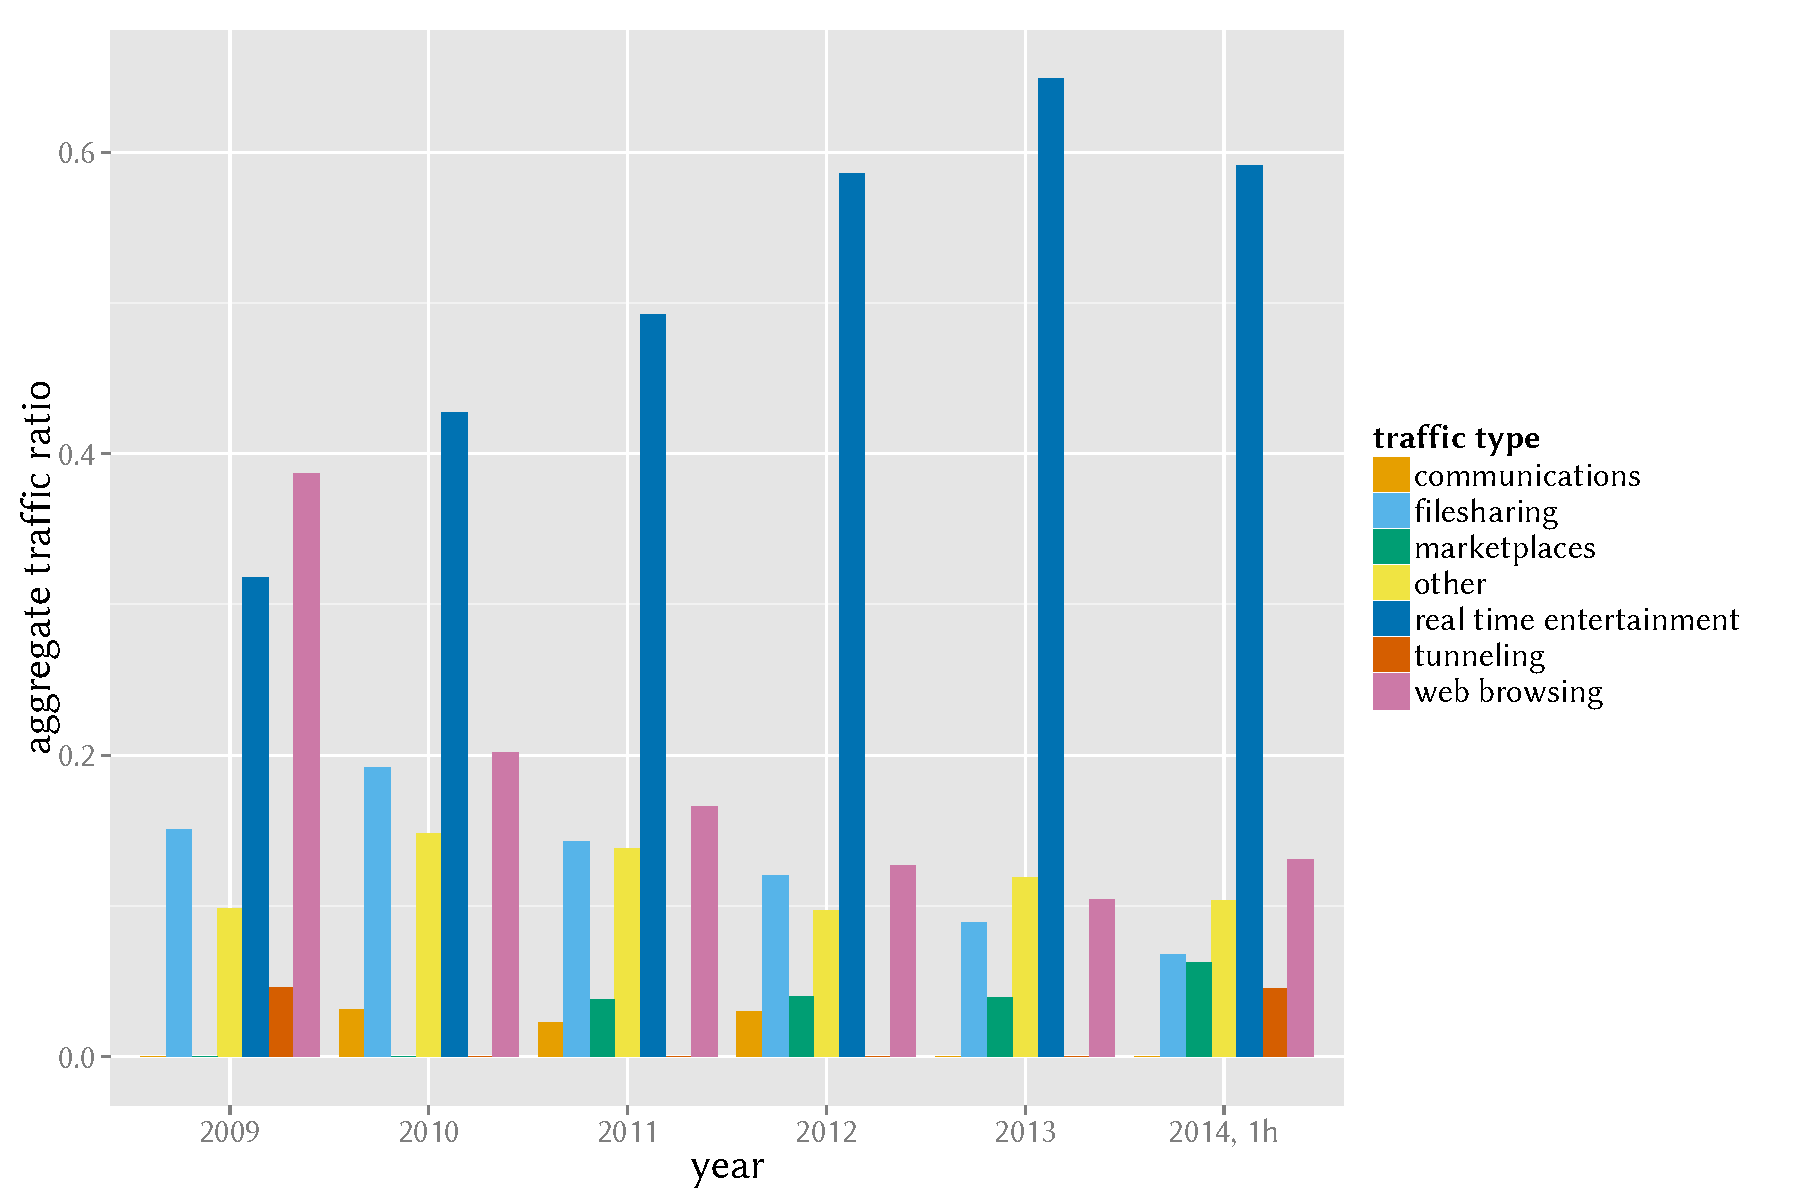
\includegraphics[width=0.9\columnwidth]{../../chapters/01-intro/images/r-netvine-phenomena-fixed.pdf}
		\caption{Traffic composition of North American peak fixed access aggregate traffic (data source:~\cite{sandvine_internetphenomena}).}
	\column{.5\textwidth}
		\begin{figure}
			\centering
			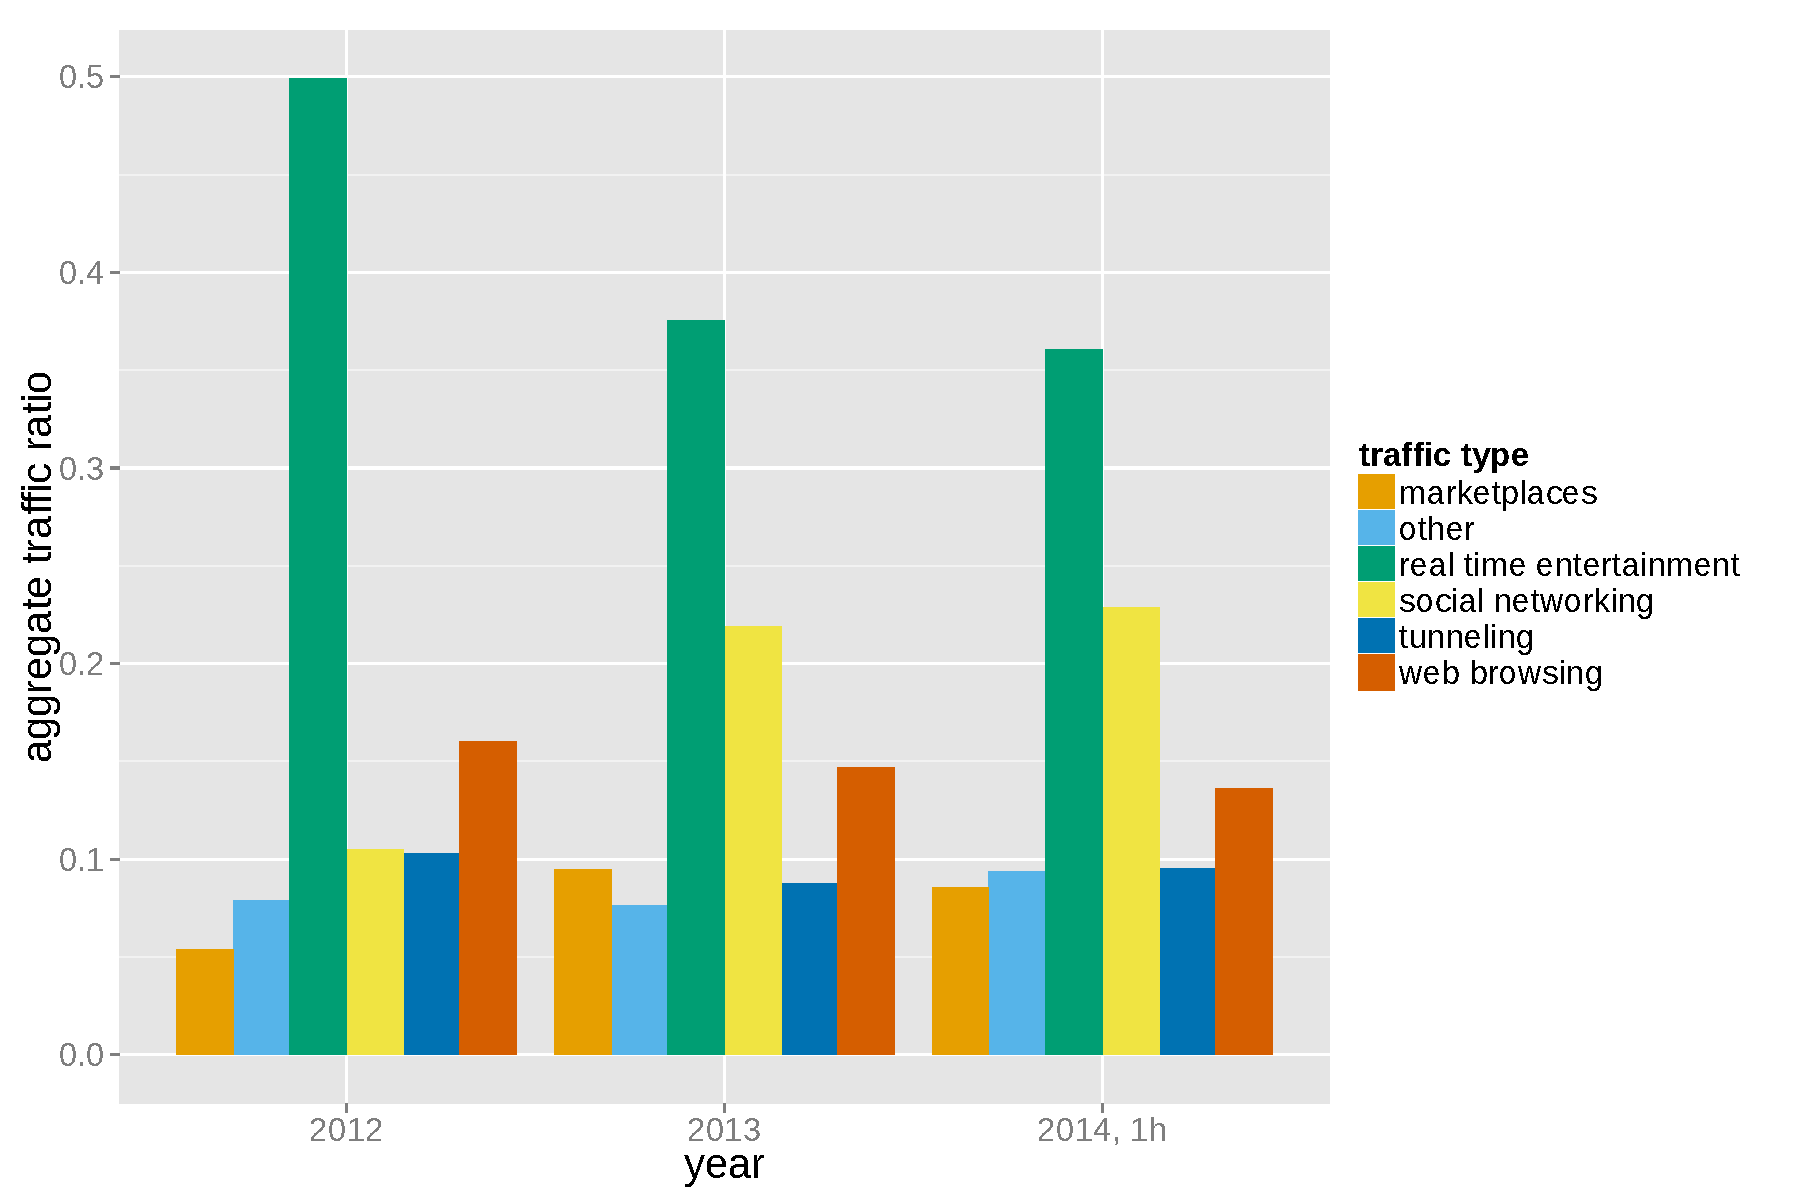
\includegraphics[width=0.9\columnwidth]{../../chapters/01-intro/images/r-netvine-phenomena-mobile.pdf}
			\caption{Traffic composition of North American peak mobile access aggregate traffic (data source:~\cite{sandvine_internetphenomena}).}
		\end{figure}
	\end{columns}

\end{figure}
\end{frame}

\begin{frame}
	\begin{figure}
		\centering
		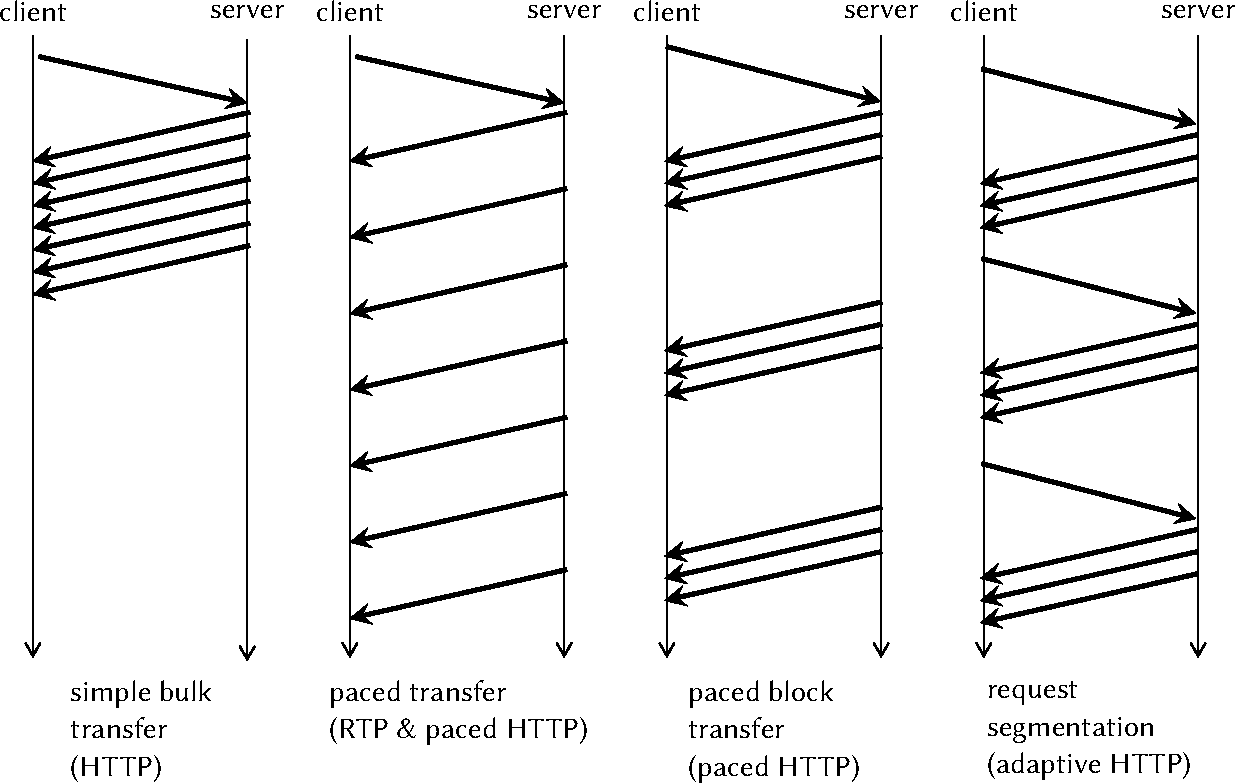
\includegraphics[height=6cm]{../../chapters/03-streaming/images/streaming-transfer-modes.pdf}
		\caption{Comparison of several possible streaming transmission modes depicting the timing of the sent packets (source:~\cite{ma2011mobile}).}
	\end{figure}
\end{frame}


\begin{frame}
	\frametitle{Protocol Classification Matrix}
{
\scriptsize
\begin{tabu}{X[0.8]XX[1.2]XXXX[0.85]} 
	\toprule
	\textbf{Protocol} & \textbf{Vertical Location of Control} & \textbf{Horizontal Location of Control} & \textbf{Reliable Transport} & \textbf{Video Type} & \textbf{Adaptivity} & \textbf{Multicast} \\ 
	\midrule
	RTP & out-of-band, application layer protocol & server-side and limited intermediary (translators and mixers) & unreliable (UDP) & low delay live streaming & server-side adaptation (transcoding) & using IGMP\\
	simple HTTP & in-band, streaming application & client-side & reliable (TCP) & stored, not live & none & emulated through CDN\\
	adaptive HTTP (e.g. DASH) & in-band, streaming application & client-side & reliable (TCP) & stored and near-live & client-side with file segmentation & emulated through CDN\\
	\bottomrule
\end{tabu}
}
\end{frame}


\begin{frame}
	\frametitle{Further Playback Strategies}

	\begin{columns}[T]
		\column{0.5\textwidth}
		\begin{figure}
			\centering
			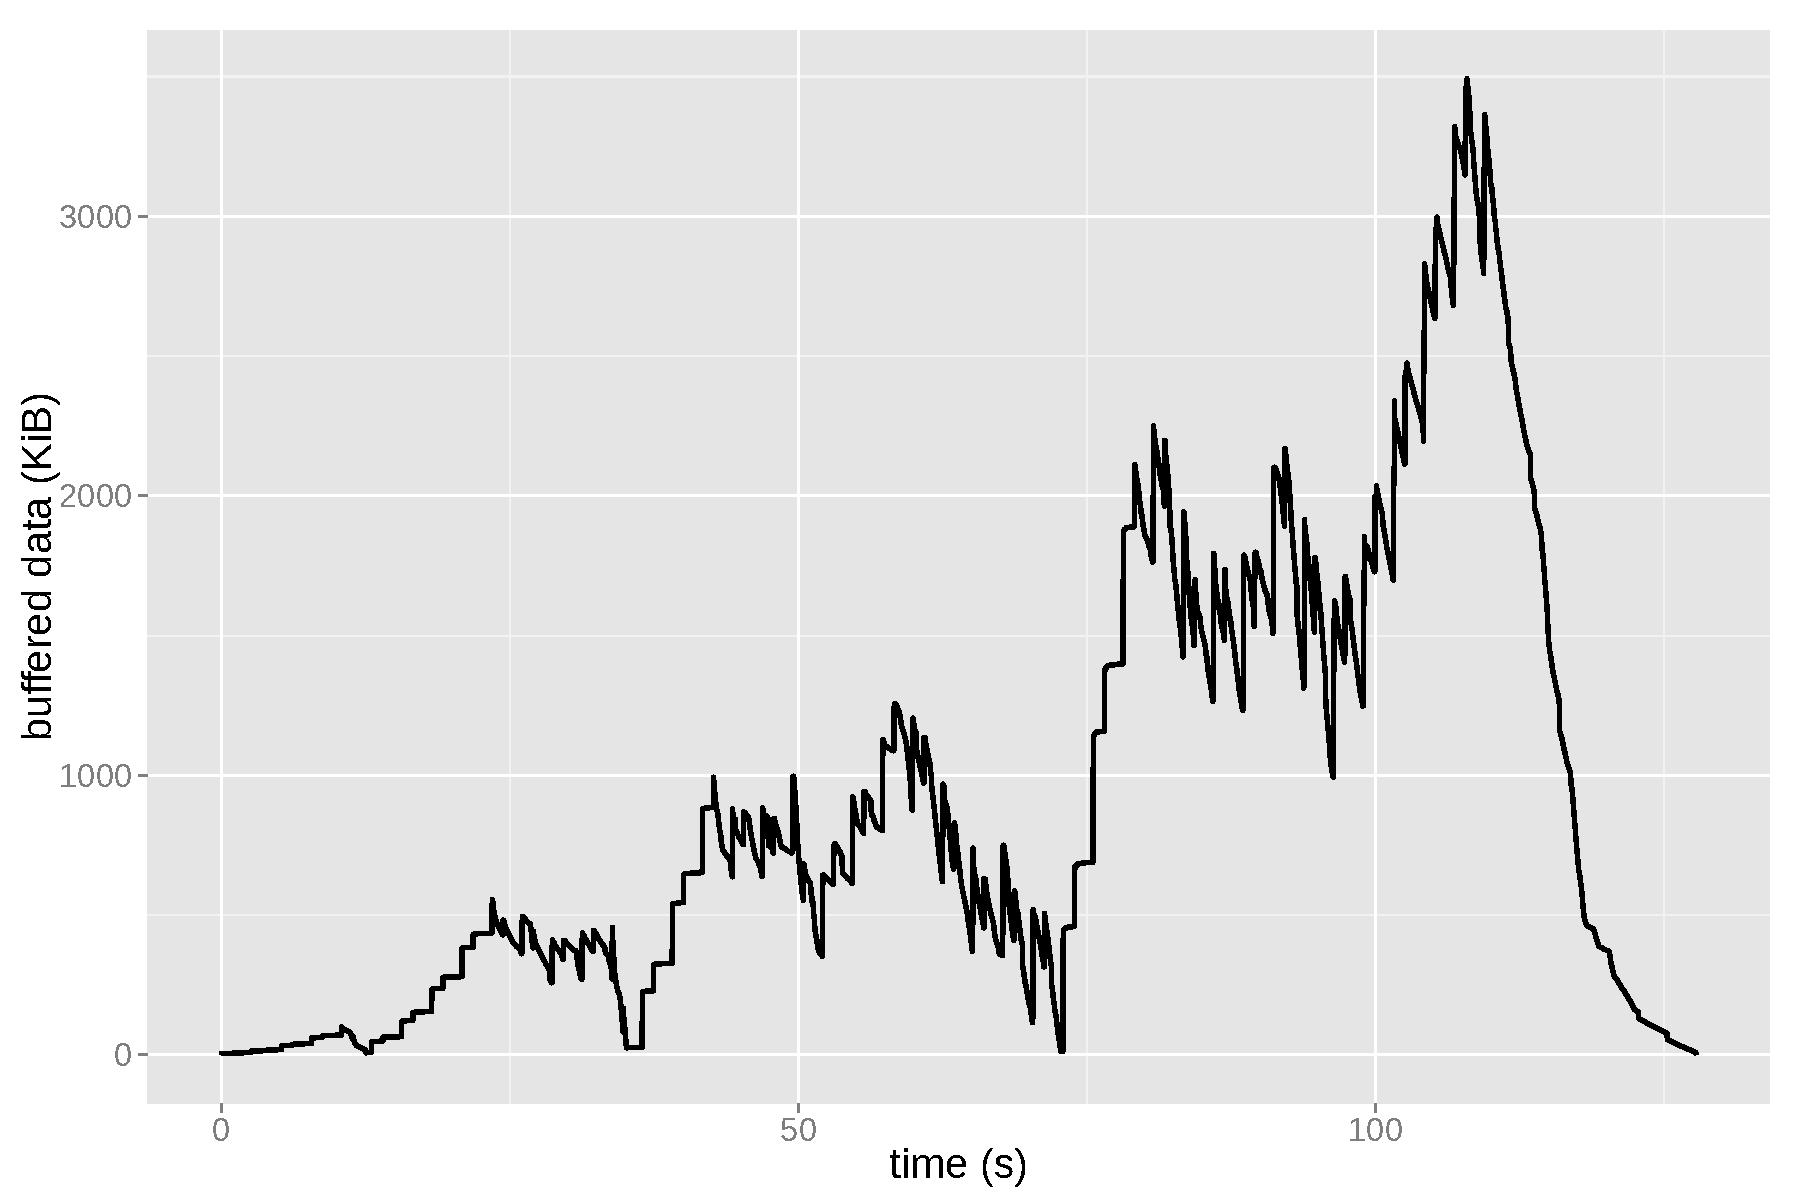
\includegraphics[width=1.0\columnwidth]{../../chapters/03-streaming/images/R-bufferlevel-flash.pdf}
			\caption{Sample buffer fill level for a \SI{5}{\second} buffered video duration threshold strategy with an additional \SI{2}{\second} initial threshold; \SI{34}{\second} total stalling.}
		\end{figure}

		\column{0.5\textwidth}
		\begin{figure}
			\centering
			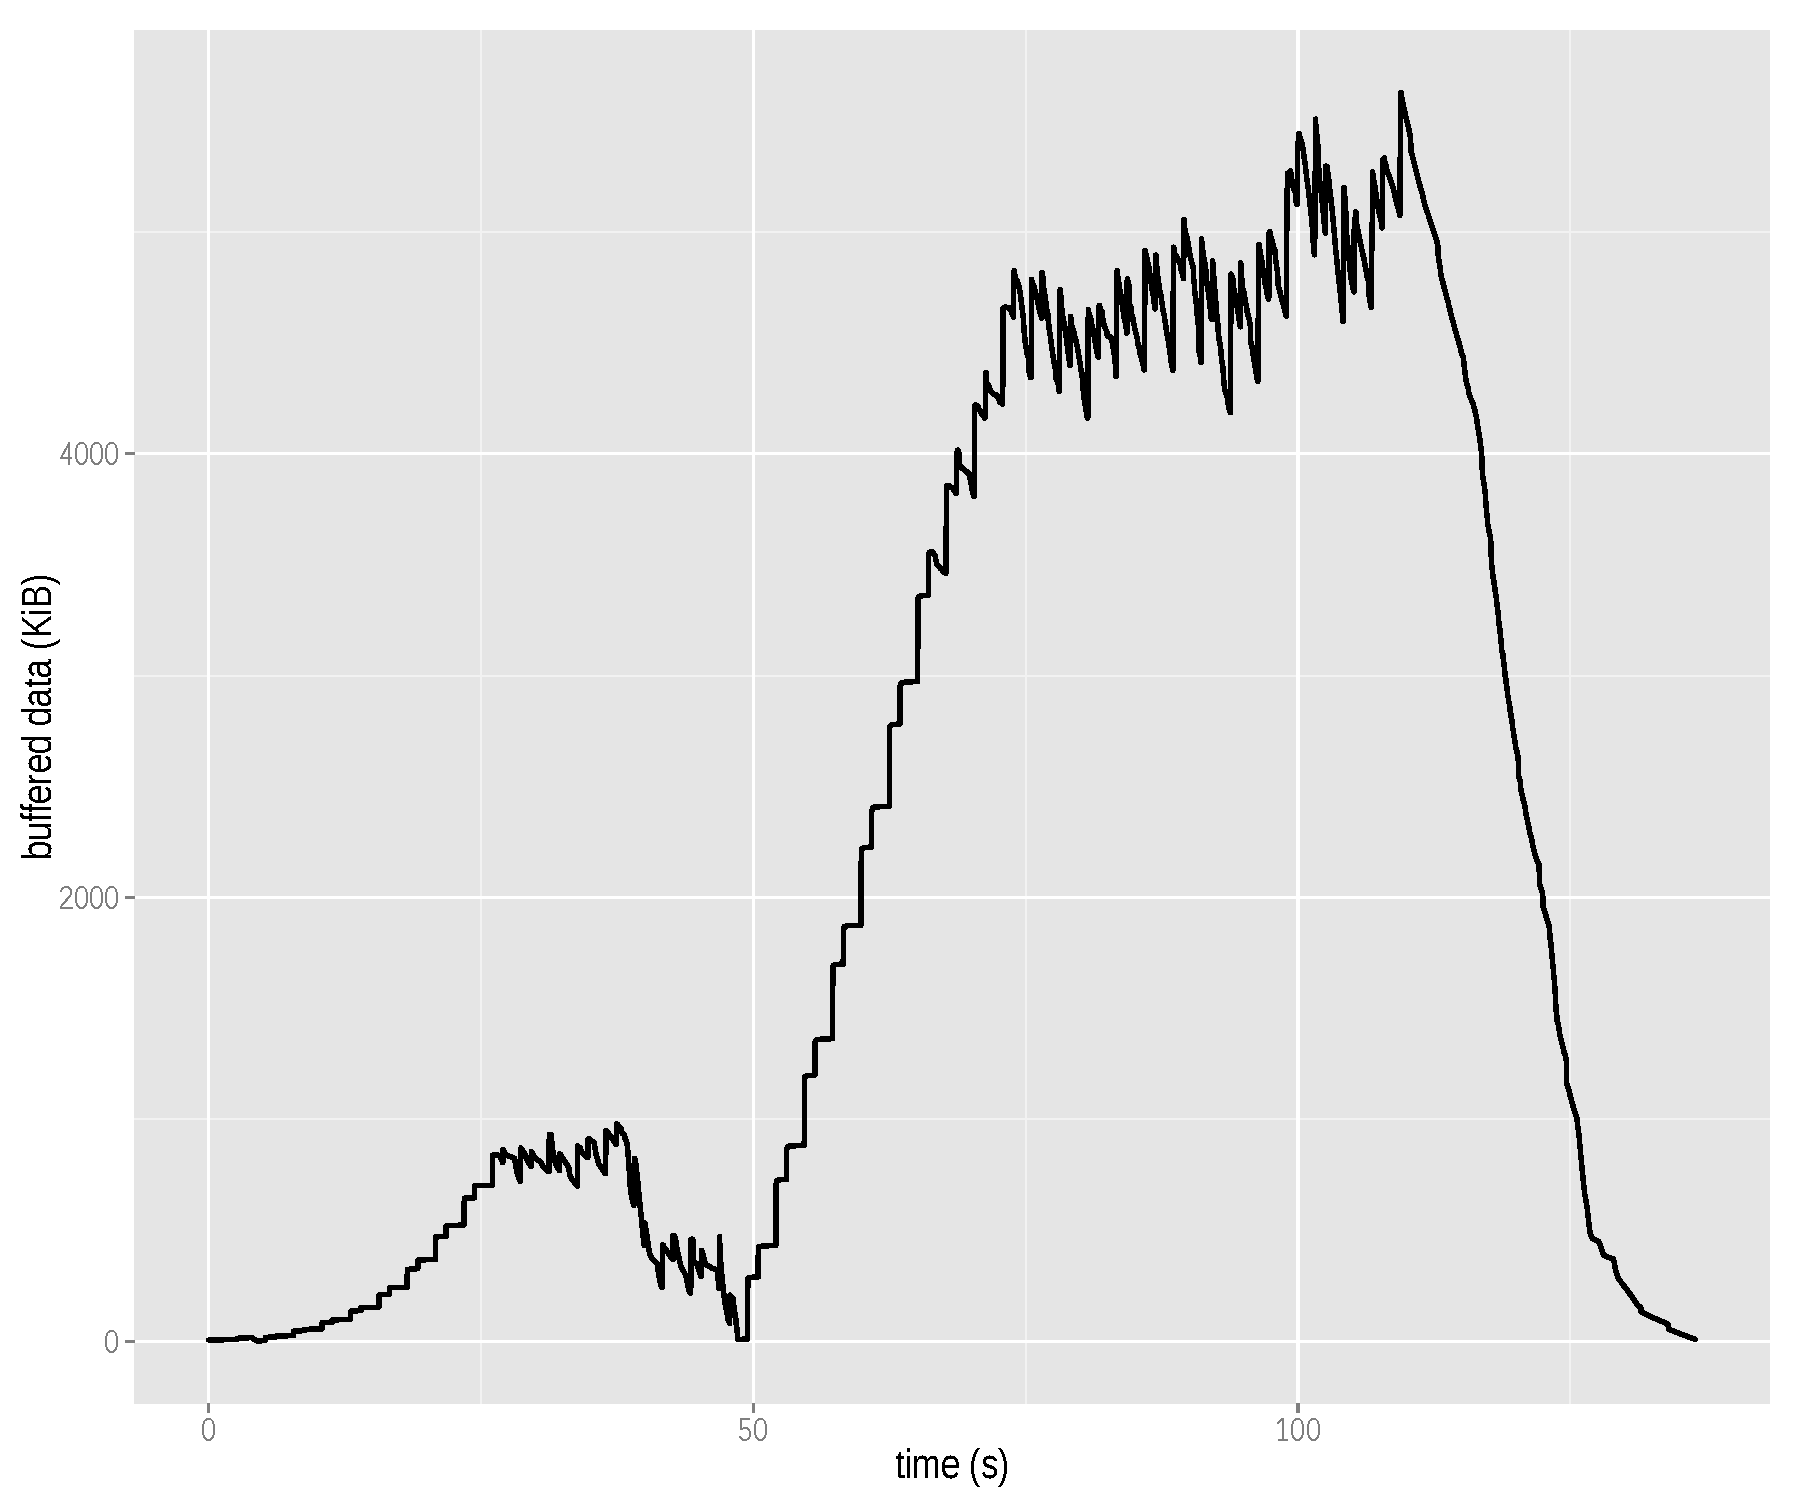
\includegraphics[width=1.0\columnwidth]{../../chapters/03-streaming/images/R-bufferlevel-firefox.pdf}
			\caption{Sample buffer fill level for the Firefox 4 strategy, \SI{44}{\second} total stalling.}
		\end{figure}
	\end{columns}
\end{frame}

\begin{frame}
	\frametitle{Firefox 4 Playback Strategy}

	\begin{algorithmic}
		\IF {$s_{MA} > v_{MA}$} 
			\STATE $c \gets ( b_b=20s \lor b_T=20s )$
		\ELSE
			\STATE $c \gets ( b_b=30s \lor b_T=30s )$
		\ENDIF
	\end{algorithmic}

	To estimate the current and future rates, the moving average of the transmission rate $s_{MA}$ and the video bitrate $v_{MA}$ are calculated. The condition $c$ Firefox uses to start and resume the playback process is given in the algorithm, with the buffered video duration $b_b$, and the duration spent buffering $b_T$.
\end{frame}

\begin{frame}
	\frametitle{Adaptive Streaming Measurement Framework}

	\begin{figure}
		\centering
		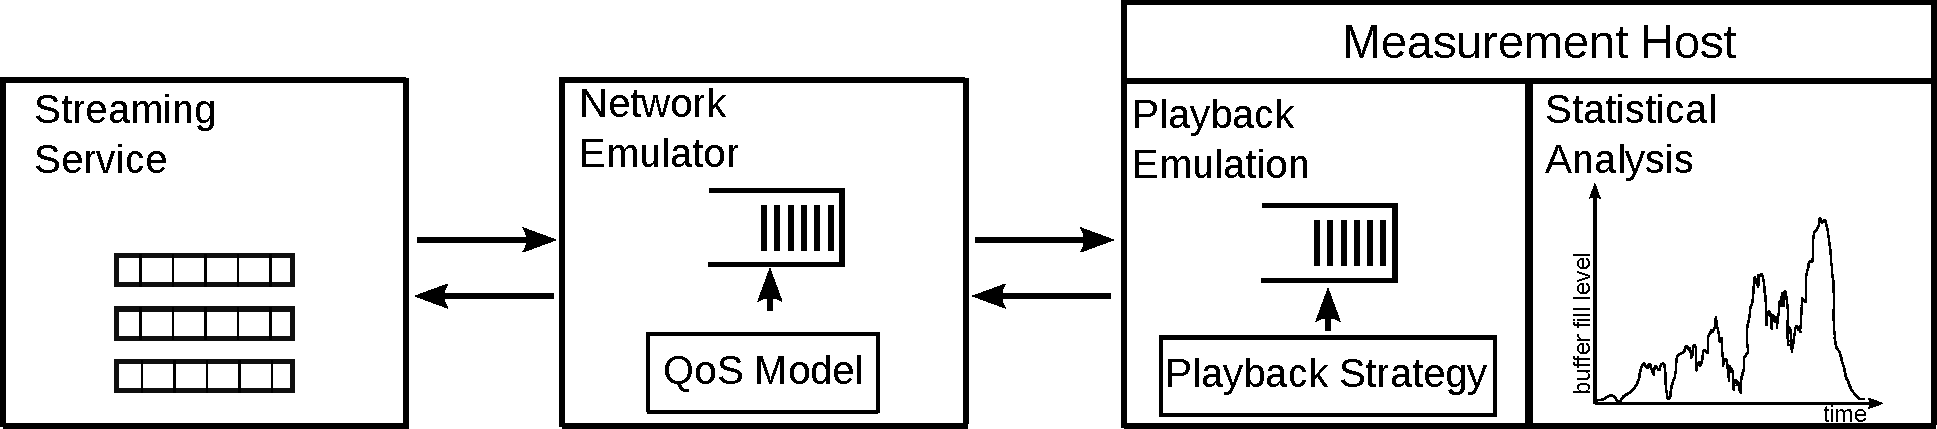
\includegraphics[height=2.5cm]{../../chapters/03-streaming/images/feedback-measurement-model.pdf}
		\caption{Overview of the measurement framework for adaptive streaming playback strategies.}
	\end{figure}
\end{frame}


\begin{frame}
	\frametitle{Latency Measurement Series}

	\begin{columns}[T]
		\column{0.5\textwidth}
		\begin{figure}
		\centering
		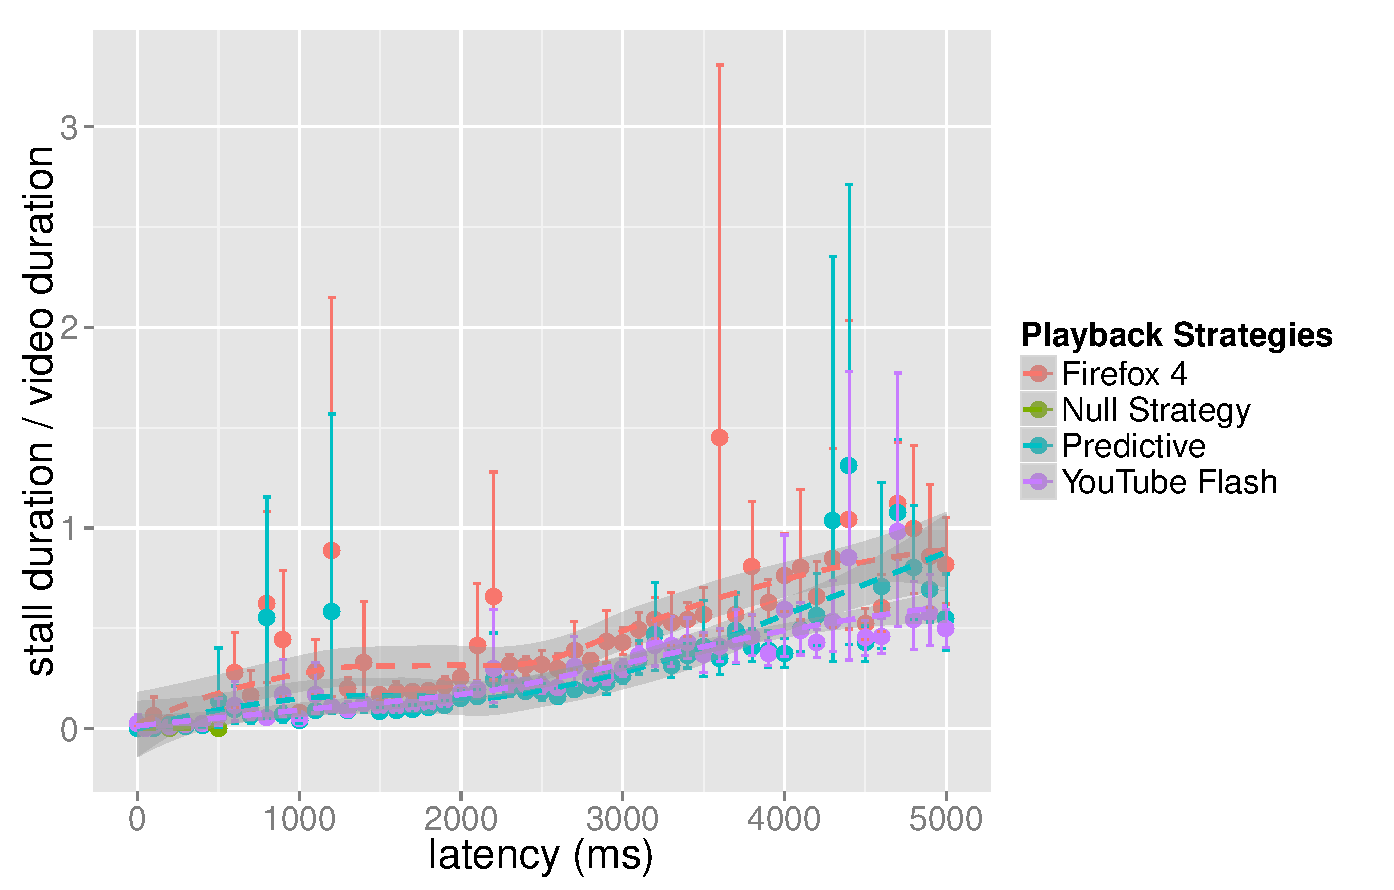
\includegraphics[width=1.0\columnwidth]{../../chapters/03-streaming/images/R-playbackemulation-stallduration-latency.pdf}
		\caption{Stalling duration in relation to transmission latency with a local polynomial least-squares fit.}
		\end{figure}

		\column{0.5\textwidth}
		\begin{figure}
		\centering
		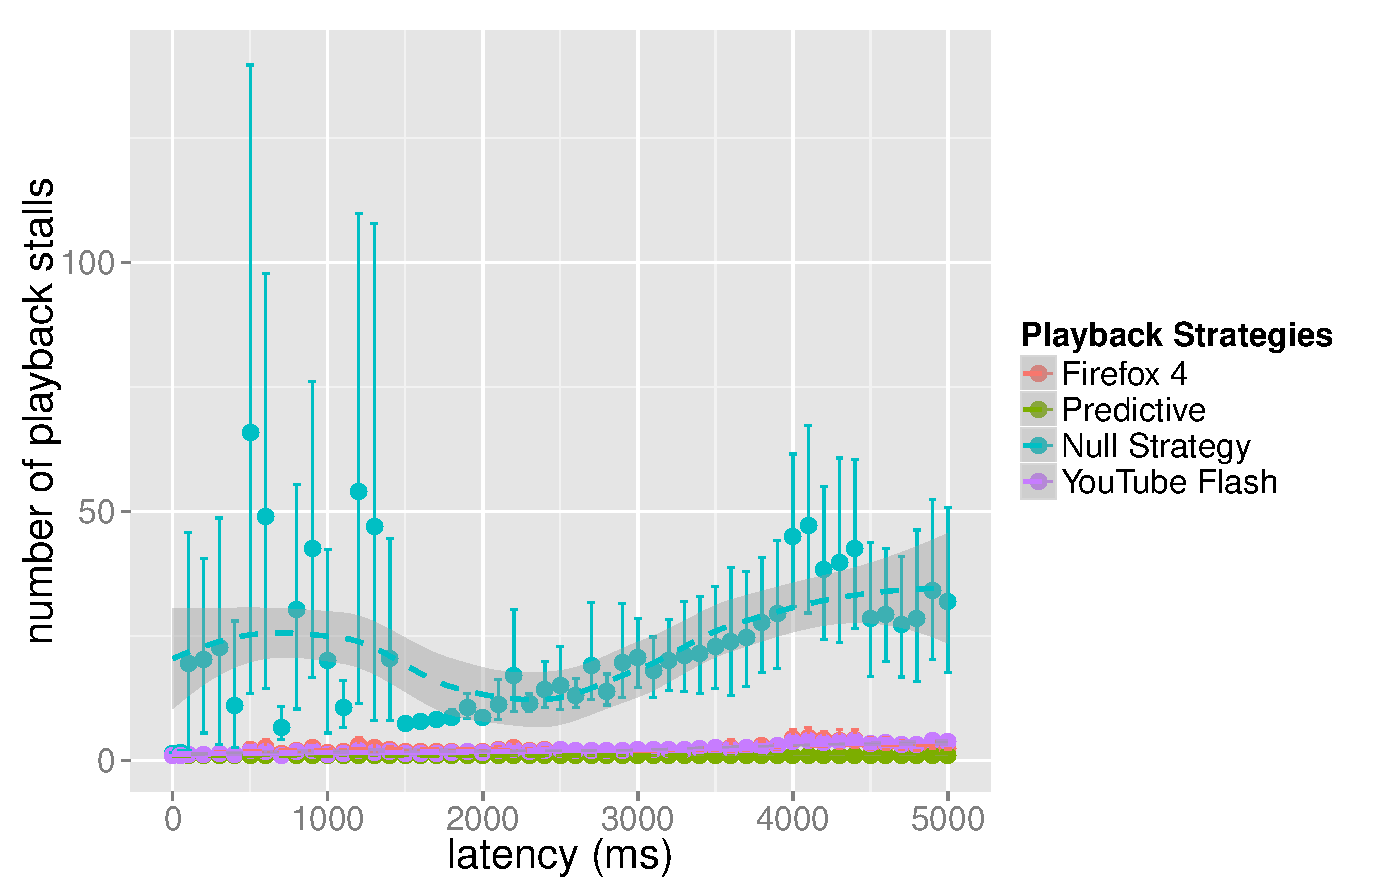
\includegraphics[width=1.0\columnwidth]{../../chapters/03-streaming/images/R-playbackemulation-stallnumber-latency.pdf}
		\caption{Number of stalls in relation to transmission latency with a local polynomial least-squares fit.}
		\end{figure}
	\end{columns}
\end{frame}

\begin{frame}
	\frametitle{Loss Measurement Series}

	\begin{columns}[T]
		\column{0.5\textwidth}
		\begin{figure}
		\centering
		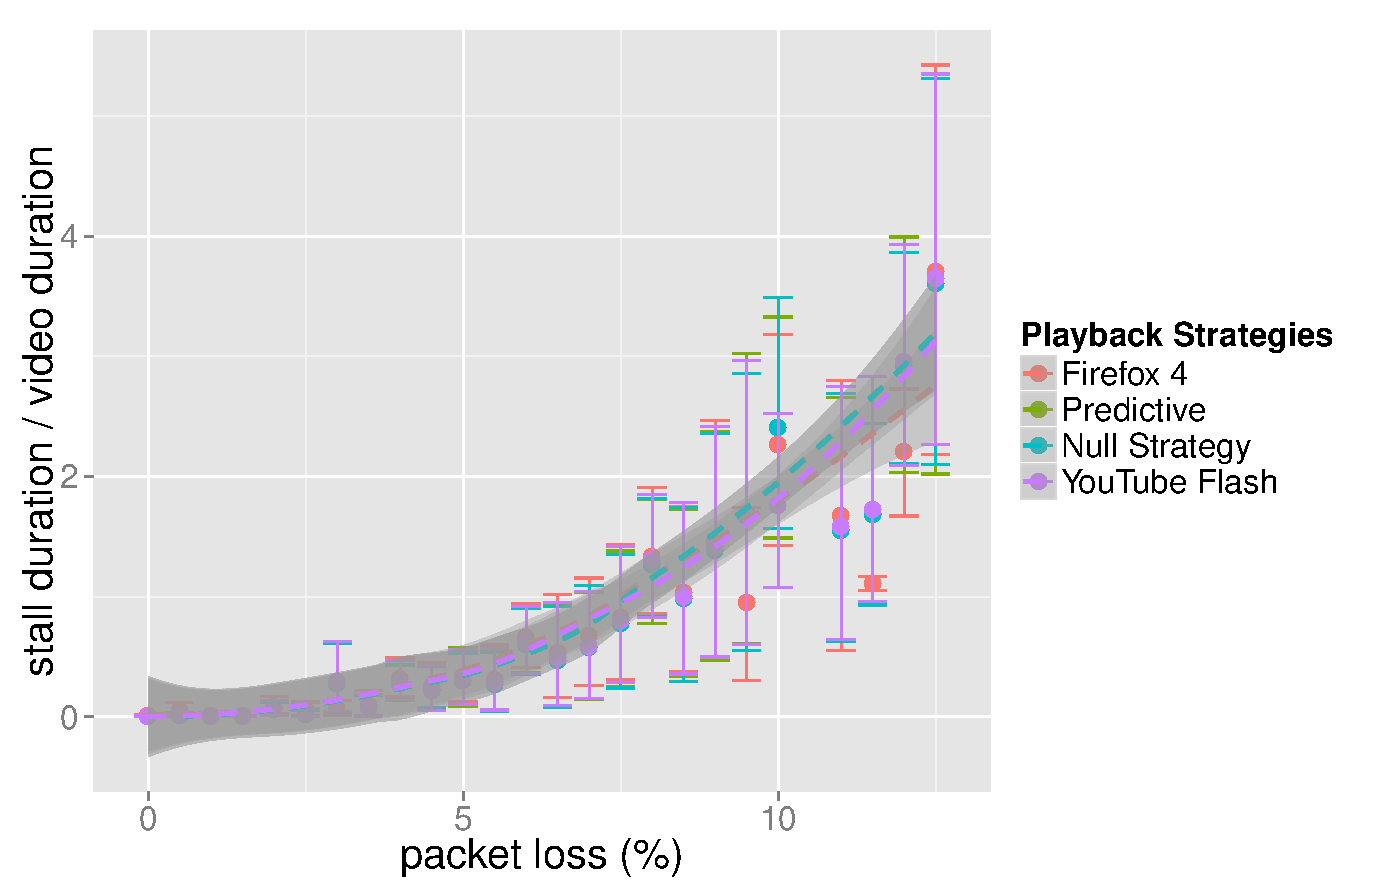
\includegraphics[width=1.0\columnwidth]{../../chapters/03-streaming/images/R-playbackemulation-stallduration-loss.pdf}
		\caption{Stalling duration in relation to the packet loss with a local polynomial least-squares fit.}
		\end{figure}

		\column{0.5\textwidth}
		\begin{figure}
			\centering
			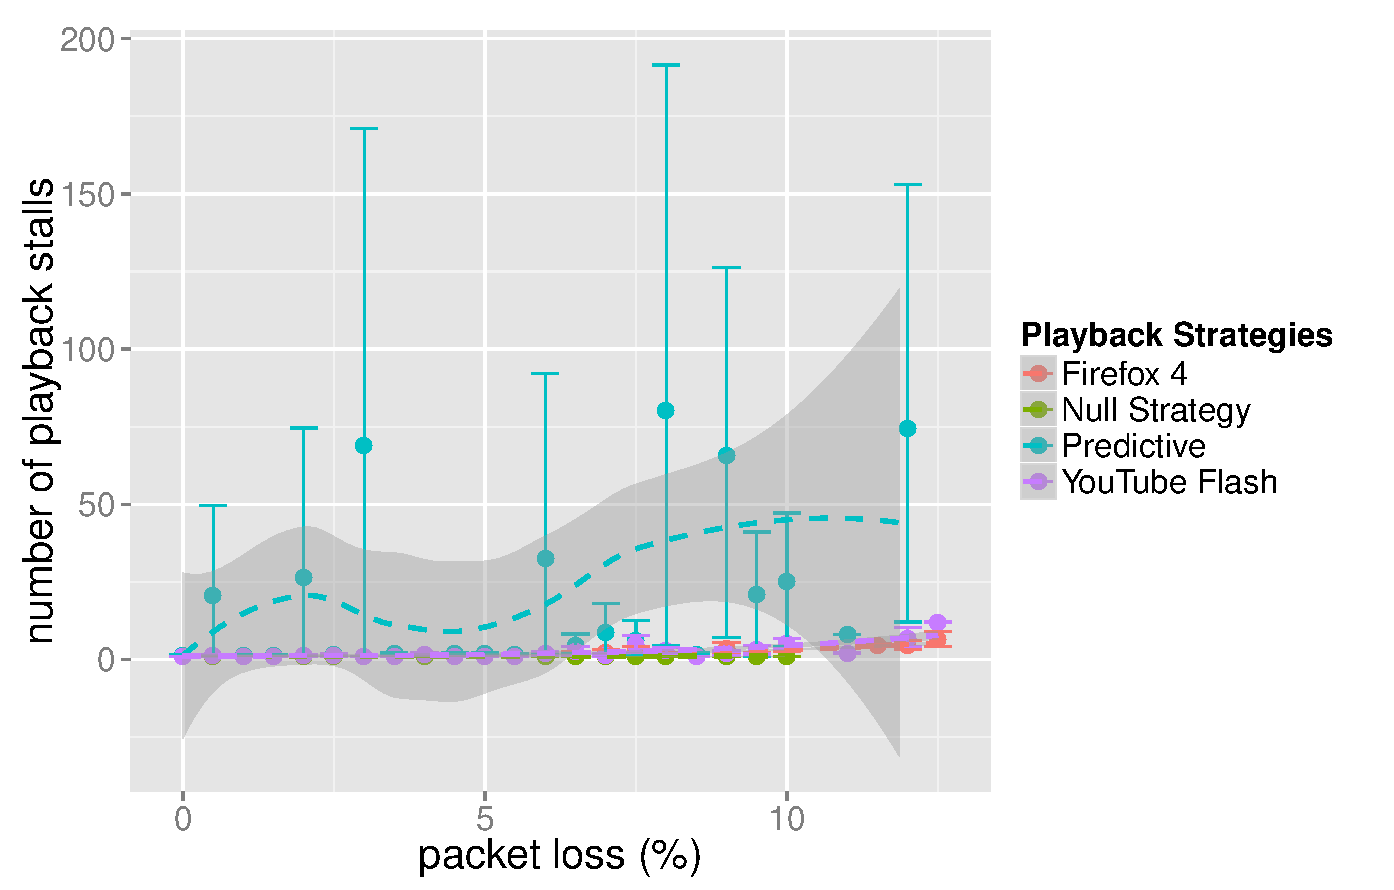
\includegraphics[width=1.0\columnwidth]{../../chapters/03-streaming/images/R-playbackemulation-stallnumber-loss.pdf}
			\caption{Number of playback stalls in relation to packet loss with local polynomial least-squares fit.}
		\end{figure}
	\end{columns}
\end{frame}

\begin{frame}
	\frametitle{Loss Measurement Series QoE}

	\begin{figure}
		\centering
		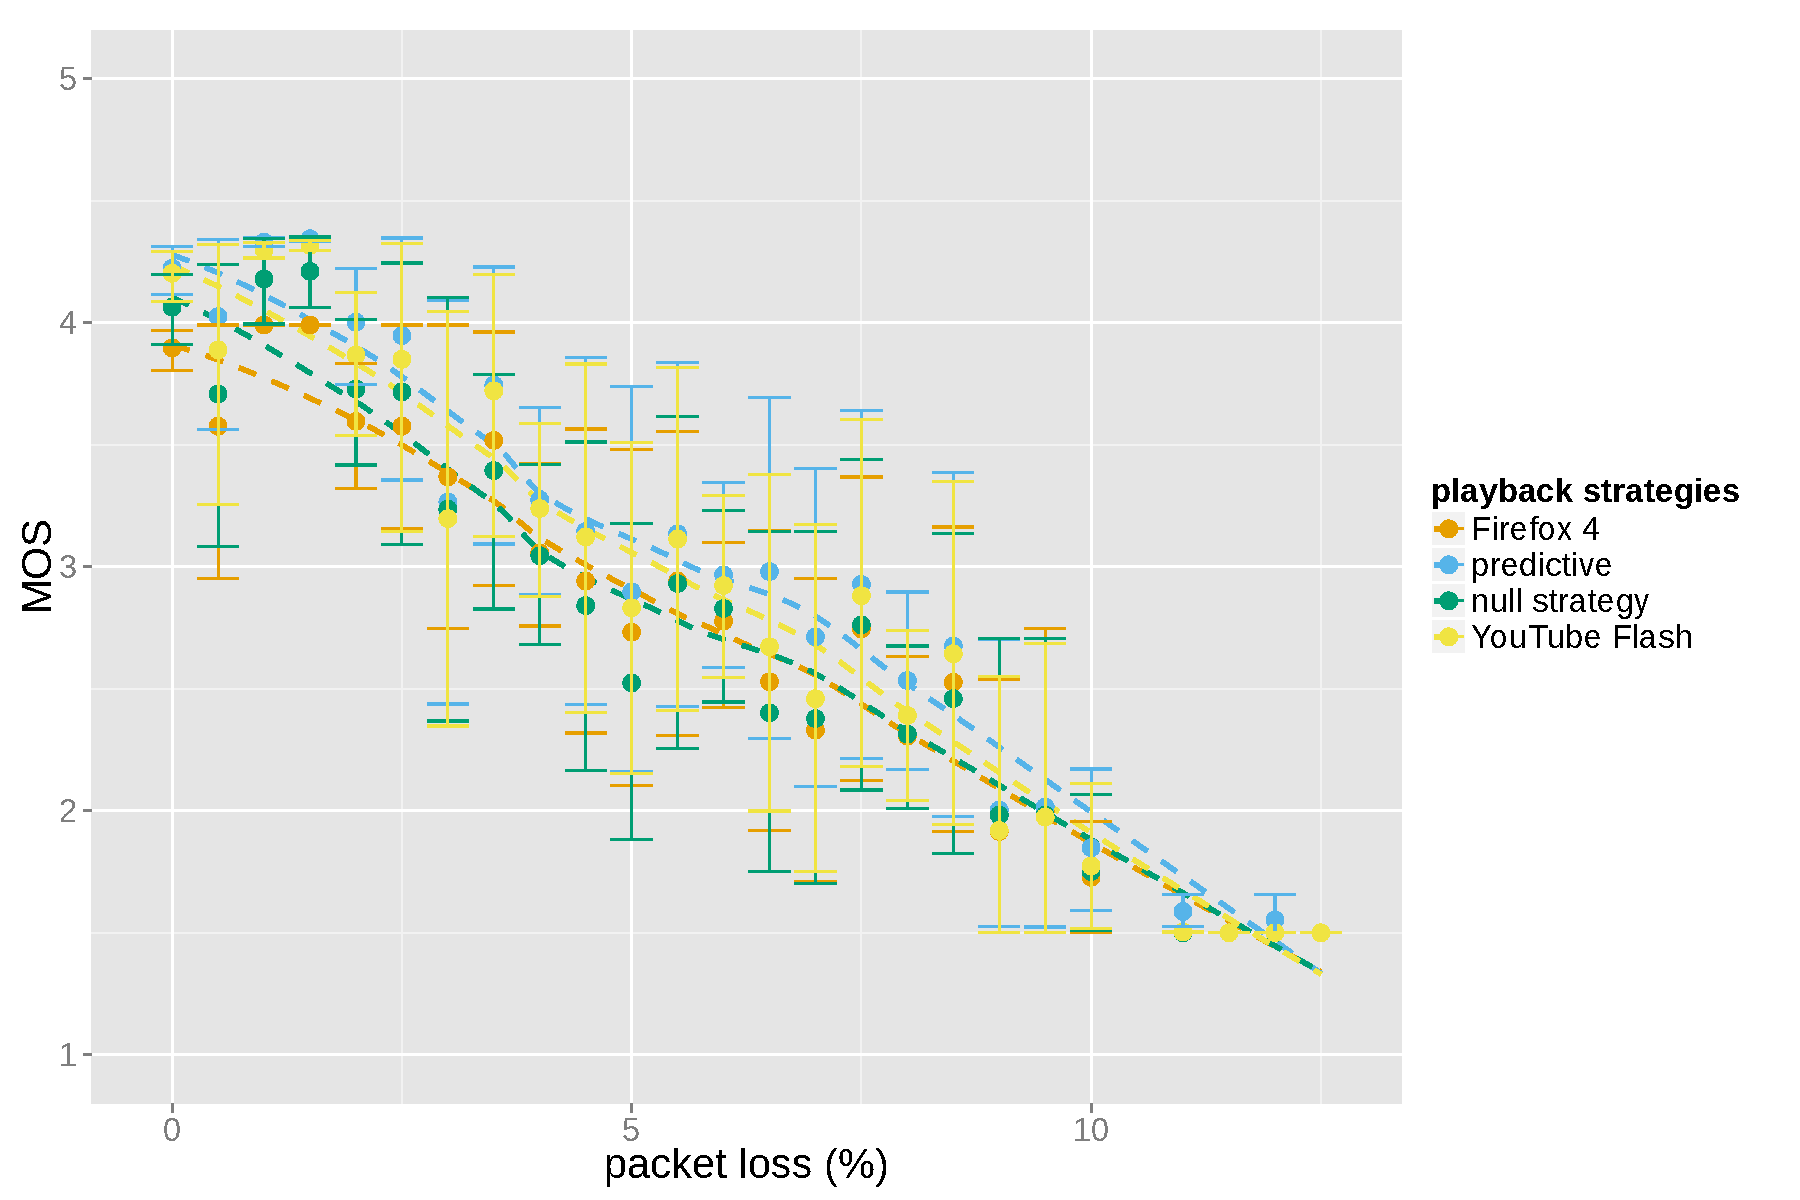
\includegraphics[height=6cm]{../../chapters/03-streaming/images/R-playbackemulation-qoe-loss.pdf}
		\caption{Calculated MOS for the loss measurement series.}
	\end{figure}
\end{frame}







\begin{frame}
	\begin{figure}
		\centering
		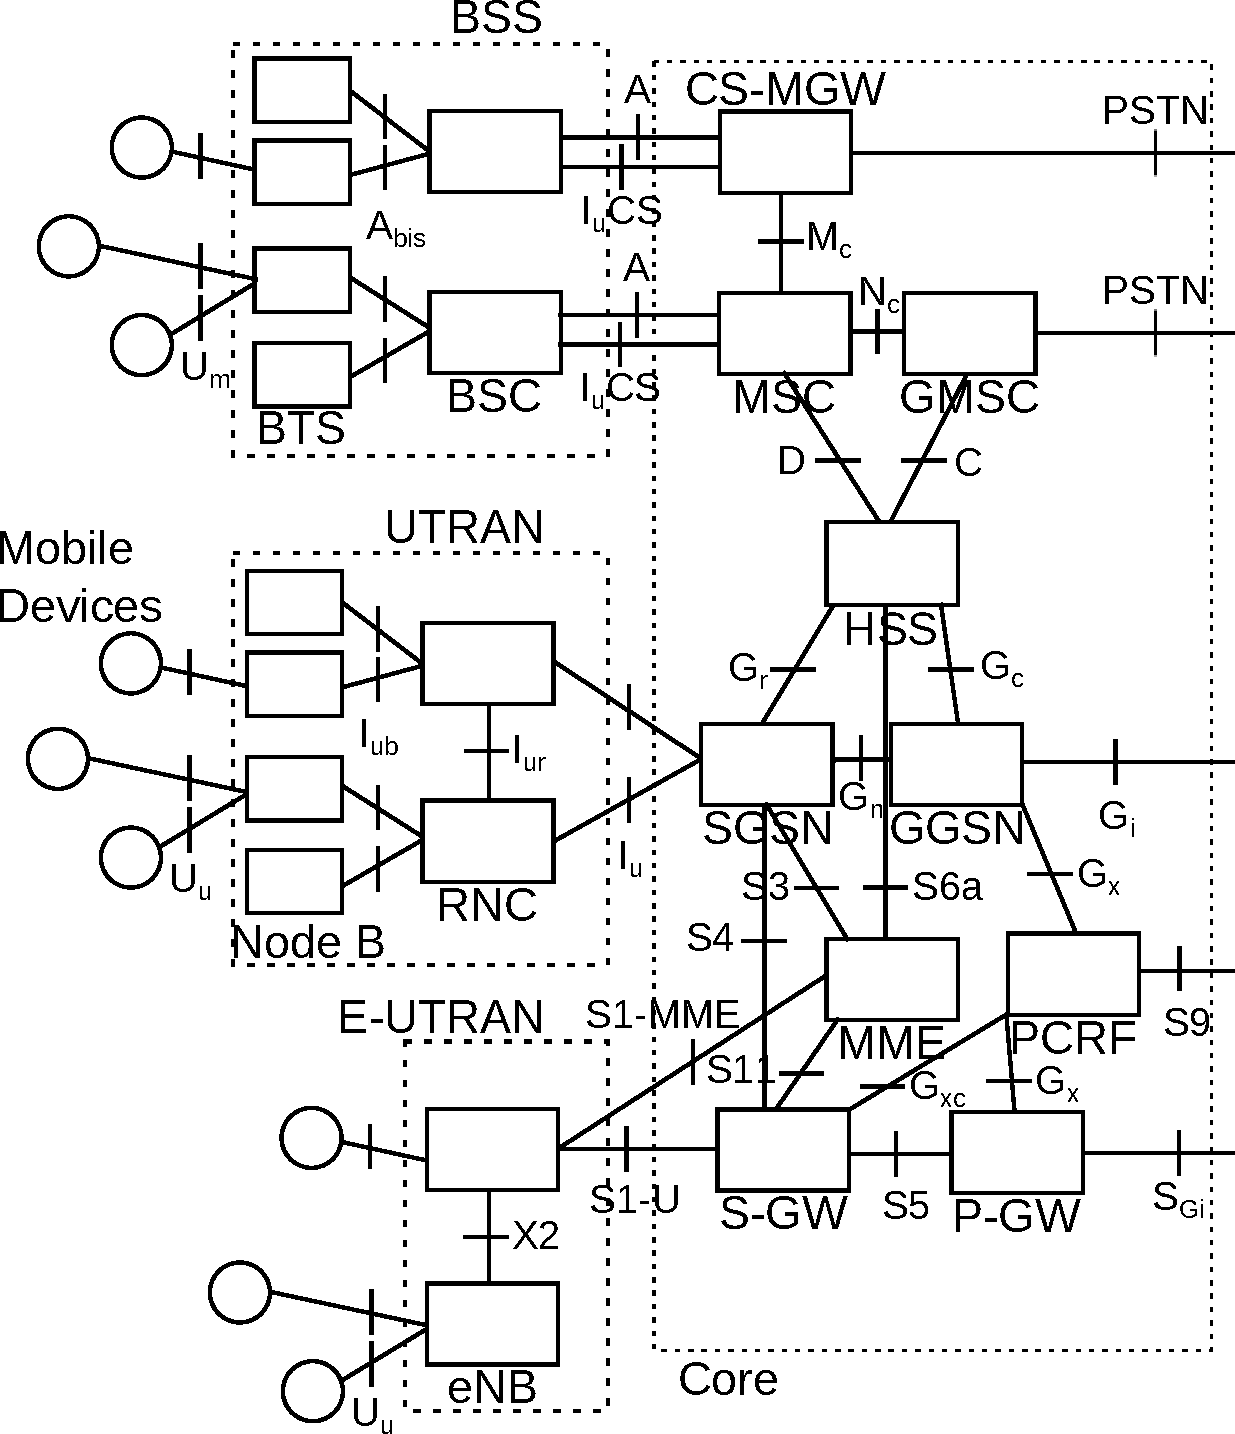
\includegraphics[height=7cm]{../../chapters/04-mobilenets/images/3gpp-physical-arch.pdf}
		\caption{Overview of a combined CS/PS GSM/UMTS/LTE architecture.}
	\end{figure}
\end{frame}


\begin{frame}
	\begin{figure}
		\centering
		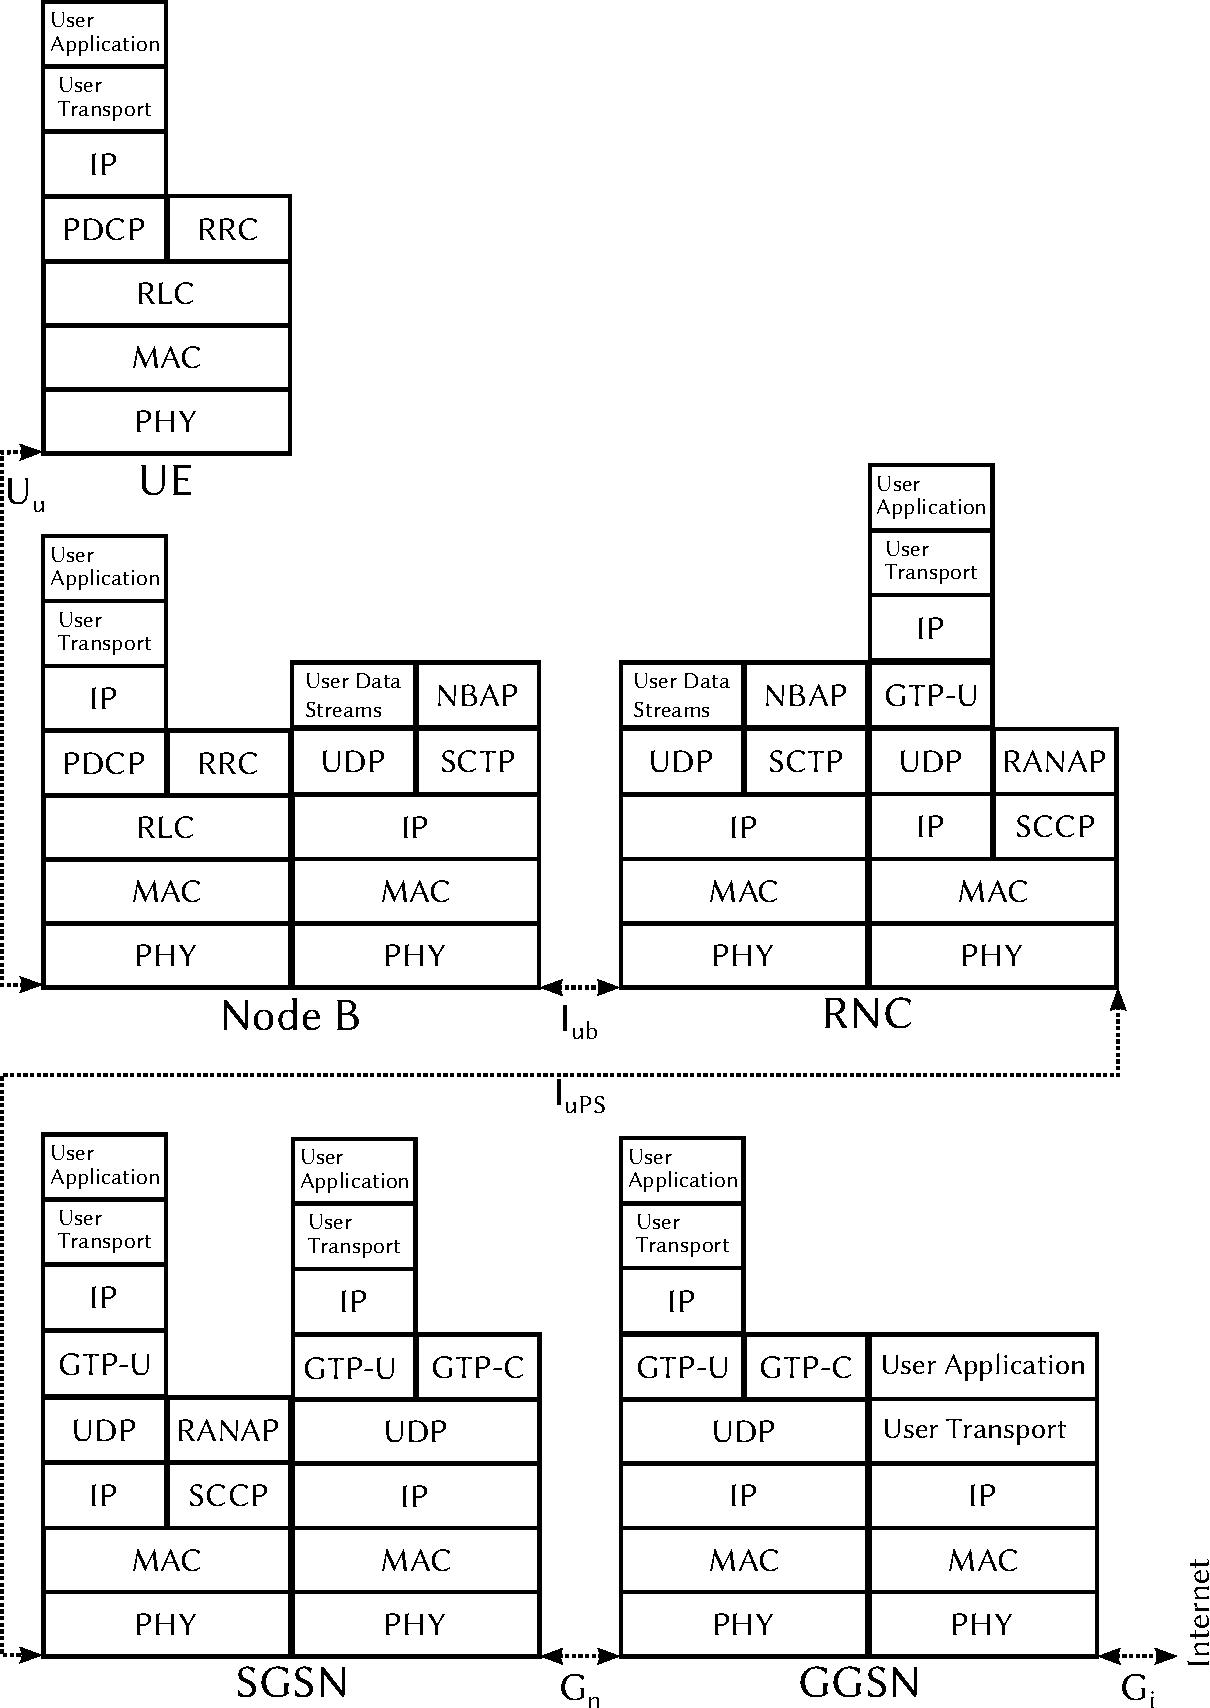
\includegraphics[height=7cm]{../../chapters/04-mobilenets/images/umts-userpath-stack.pdf}
		\caption{Simplified control plane and user plane IP-based protocol stacks on the user traffic path through the mobile network.}
	\end{figure}
\end{frame}


\begin{frame}
	\begin{figure}
		\centering
		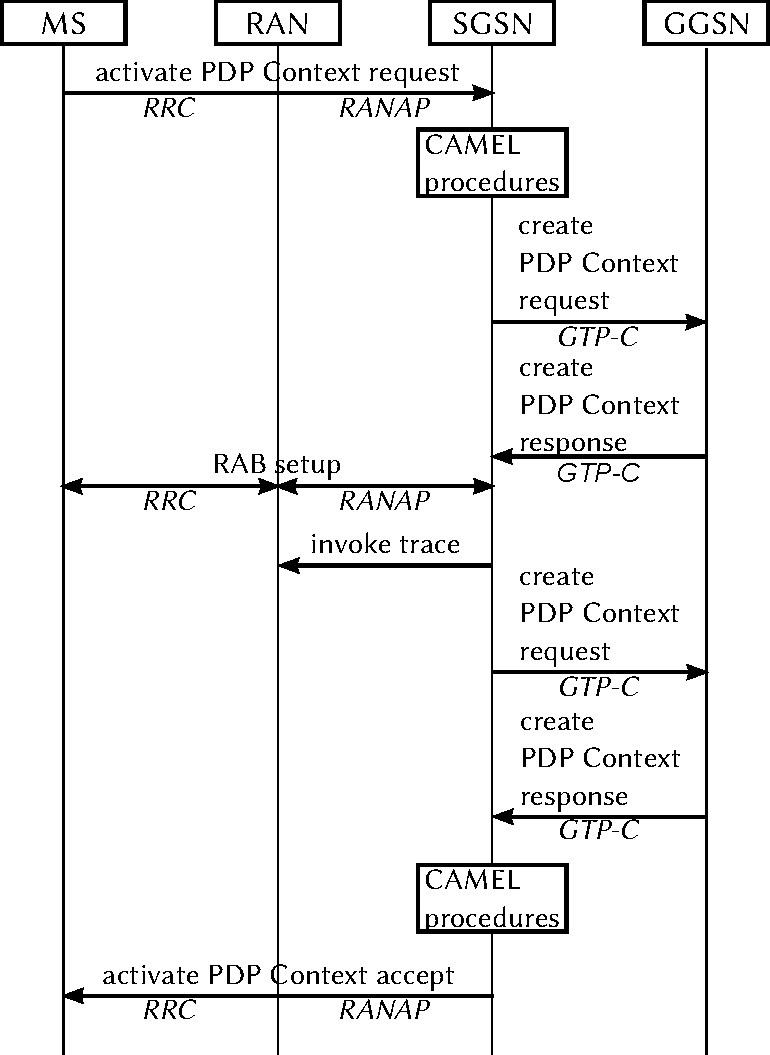
\includegraphics[height=7cm]{../../chapters/04-mobilenets/images/pdp-context-activation-procedure.pdf}
		\caption{PDP Context activation procedure signaling interaction diagram for UMTS, including involved signaling protocols.}
	\end{figure}
\end{frame}

\begin{frame}
	\begin{figure}
		\scriptsize
		\begin{tabu}{X[1]|X[1]|X[1]|X[1]|X[1]|X[1]|X[1]|X[1]|X[1]|}
		\multicolumn{1}{c}{} & \multicolumn{8}{c}{\textbf{Bits}} \\
		\textbf{Octets} & \textbf{8} & \textbf{7} & \textbf{6} & \textbf{5} & \textbf{4} & \textbf{3} & \textbf{2} & \textbf{1} \\ 
		\cline{2-9} \textbf{1} & \multicolumn{3}{c|}{Version}  & 1 & 0 & E & S & PN \\ 
		\cline{2-9} \textbf{2} & \multicolumn{8}{c|}{Message Type}  \\ 
		\cline{2-9} \textbf{3} & \multicolumn{8}{c|}{\multirow{2}{*}{Length}}  \\ 
					\textbf{4} & \multicolumn{8}{c|}{}  \\ 
		\cline{2-9} \textbf{5} & \multicolumn{8}{c|}{\multirow{4}{*}{Tunnel Endpoint Identifier}} \\ 
					\textbf{6} & \multicolumn{8}{c|}{} \\ 
					\textbf{7} & \multicolumn{8}{c|}{} \\ 
					\textbf{8} & \multicolumn{8}{c|}{} \\ 
		\cline{2-9} \textbf{9} & \multicolumn{8}{c|}{\multirow{2}{*}{Sequence Number}} \\
					\textbf{10} & \multicolumn{8}{c|}{} \\
		\cline{2-9}	\textbf{11} & \multicolumn{8}{c|}{N-PDU} \\
		\cline{2-9} \textbf{12} & \multicolumn{8}{c|}{Next Extension Header Type} \\
		\cline{2-9}
		\end{tabu} 
		\caption{General \SI{12}{\byte} GTP header format.}
	\end{figure}
\end{frame}

\begin{frame}
	\begin{table}
	\tiny
	\caption{All IE in a Create PDP Context request and size thereof for IPv4 network and user traffic only. The denoted sizes exclude the first message type byte.}
		\begin{tabu} to 0.49\textwidth{X[2.5]X[1.2]X[0.7]}
			\toprule
			\textbf{IE} & \textbf{Presence} & \textbf{Size}\\
			\midrule
			IMSI & cond. & \SI{8}{\byte} \\ 
			RAI & opt. & \SI{6}{\byte} \\
			Recovery & opt. & \SI{1}{\byte} \\
			Selection mode	& cond. & \SI{1}{\byte} \\
			TEID Data I & mand. & \SI{4}{\byte} \\
			TEID Control Plane & cond. & \SI{4}{\byte} \\
			NSAPI & mand. & \SI{1}{\byte} \\
			Linked NSAPI & cond. & \SI{1}{\byte} \\
			Charging Characteristics & cond. & \SI{2}{\byte} \\
			Trace Reference & opt. & \SI{2}{\byte} \\
			Trace Type & opt. & \SI{2}{\byte} \\
			End User Address & cond. & \SI{8}{\byte} \\
			APN & cond. & max \SI{102}{\byte} \\ 
			PCO & opt. & max \SI{255}{\byte} \\ 
			SGSN signaling address & mand.  & \SI{6}{\byte} \\
			SGSN user traffic address & mand. & \SI{6}{\byte} \\ 
			MSISDN & cond. & max \SI{17}{\byte} \\ 
			QoS Profile & mand. & max \SI{257}{\byte} \\
			\bottomrule
		\end{tabu}%
		\raisebox{0.63mm}{\begin{tabu} to 0.49\textwidth{X[2.5]X[1.2]X[0.7]}
			\toprule
			\textbf{IE} & \textbf{Presence} & \textbf{Size} \\
			\midrule
			TFT & cond. & max \SI{257}{\byte} \\ 
			Trigger Id & opt. & var. \\ 
			OMC Identity & opt. & var. \\ 
			Common Flags & opt. & \SI{3}{\byte} \\
			APN Restriction & opt. & \SI{3}{\byte} \\
			RAT & opt. & \SI{3}{\byte} \\
			User Location Information & opt. & \SI{10}{\byte} \\
			MS Time Zone & opt. & \SI{4}{\byte} \\
			IMEI (SV) & cond. & \SI{10}{\byte} \\
			CAMEL Charging Information Container & opt. & var. \\
			Additional Trace Info & opt. & \SI{11}{\byte} \\
			Correlation-ID & opt. & \SI{3}{\byte} \\
			Evolved Allocation Retention Priority I & opt. & \SI{3}{\byte} \\
			Extended Common Flags & opt. & \SI{3}{\byte} \\ 
			User CSG Information & opt. & \SI{10}{\byte} \\
			APN-AMBR & opt.  & \SI{11}{\byte} \\
			Signaling Priority Indication & opt. & \SI{3}{\byte} \\ 
			Private Extension & opt. & var. \\
			\bottomrule
		\end{tabu}}
	\end{table}
\end{frame}

\begin{frame}
	\begin{columns}[T]
		\column{0.5\textwidth}
		\begin{figure}
			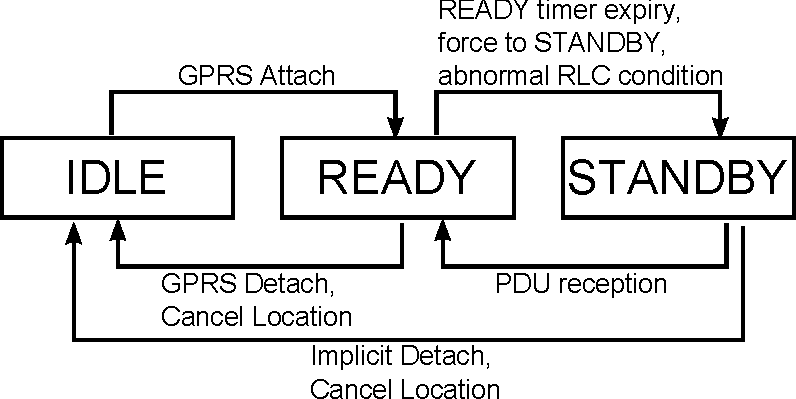
\includegraphics[width=\columnwidth]{../../chapters/04-mobilenets/images/mm-2g-state-model.pdf}
			\caption{SGSN MM state machines for 2G radio access as defined in \cite[Section~6.1]{3gpp.23.060}.}
		\end{figure}

		\column{0.5\textwidth}
		\begin{figure}
			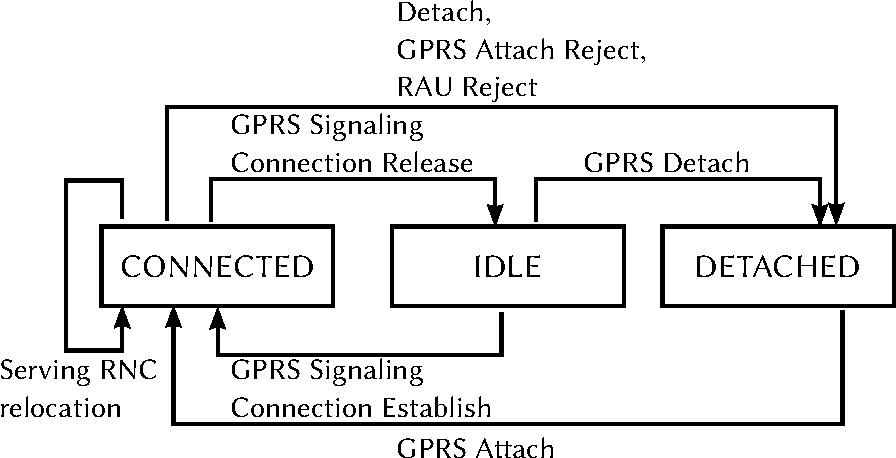
\includegraphics[width=\columnwidth]{../../chapters/04-mobilenets/images/mm-3g-state-model.pdf}
			\caption{SGSN MM state machines for 3G radio access as defined in \cite[Section~6.1]{3gpp.23.060}.}
		\end{figure}
	\end{columns}
\end{frame}

\begin{frame}
	\begin{columns}[T]
		\column{0.5\textwidth}
		\begin{figure}
			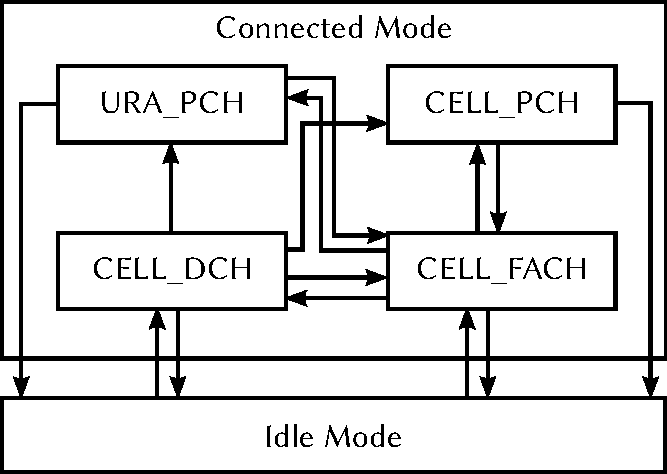
\includegraphics[width=\columnwidth]{../../chapters/04-mobilenets/images/rrc-state-model.pdf}
			\caption{RRC State Model as per \cite[Section~7.1]{3gpp.25.331}.}
		\end{figure}

		\column{0.5\textwidth}
		\begin{figure}
			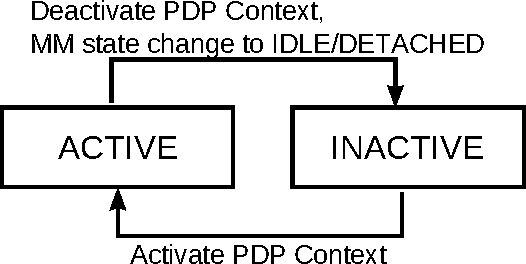
\includegraphics[width=\columnwidth]{../../chapters/04-mobilenets/images/pdp-state-model.pdf}
			\caption{PDP State Model defined in \cite[Section~9]{3gpp.23.060}.}
		\end{figure}
	\end{columns}
\end{frame}

\begin{frame}
	\begin{table}
		\caption{Relative TAC statistics.}
		\scriptsize
		\begin{tabu}{XX[r]}
			\toprule
			\textbf{Type} & \textbf{Relative number of devices with an entry in the TAC dataset}\\ 
			\midrule
			Total number of flows & \SI{99.72}{\percent} \\
			Ratio of total traffic & \SI{99.97}{\percent} \\
			Total number of tunnels & \SI{87.57}{\percent} \\
			Total number of GTP signaling messages & \SI{90.95}{\percent} \\
			Number of distinct UEs & \SI{80.93}{\percent} \\ 
			\bottomrule
		\end{tabu}
	\end{table}
\end{frame}

\begin{frame}
	\begin{table}
	\scriptsize
	\caption{Relative device-discriminated traffic statistics extracted from the dataset.}
		\begin{tabu}{X[1.4]X[r]X[r]X[r]X[1.2,r]X[r]}
		\toprule
		& \textbf{Flows} & \textbf{Traffic} & \textbf{Tunnels} & \textbf{GTP message pairs} & \textbf{Devices}\\ 
		\midrule
		\multicolumn{2}{c}{\textbf{By device type}}       &             &             &             &           \\
		% In TAC DB      & $99.72\%$   & $99.97\%$   & $87.57\%$   & $90.95\%$   & $80.93\%$ \\
		Smartphones      & $20.58\%$   & $12.81\%$   & $60.31\%$   & $75.99\%$   & $37.97\%$ \\
		Regular phones   & $0.26\%$    & $0.37\%$    & $5.40\%$    & $0.94\%$    & $9.25\%$  \\
		3G dongles & $66.55\%$   & $75.12\%$   & $12.71\%$   & $9.53\%$    & $25.10\%$ \\
		\midrule
		\multicolumn{2}{c}{\textbf{By OS}}       &             &             &             &           \\
		Android          & $10.82\%$   & $6.48\%$    & $14.33\%$   & $43.33\%$   & $14.01\%$ \\
		iOS              & $7.22\%$    & $4.47\%$    & $18.91\%$   & $20.35\%$   & $7.94\%$  \\
		Symbian          & $1.02\%$    & $1.09\%$    & $21.17\%$   & $4.51\%$    & $12.97\%$ \\
		Blackberry OS    & $0.07\%$    & $0.10\%$    & $2.17\%$    & $2.60\%$    & $1.48\%$  \\
		\bottomrule
		\end{tabu}
	\end{table}
\end{frame}

\begin{frame}
	\begin{columns}[T]
		\column{0.5\textwidth}
		\begin{figure}
			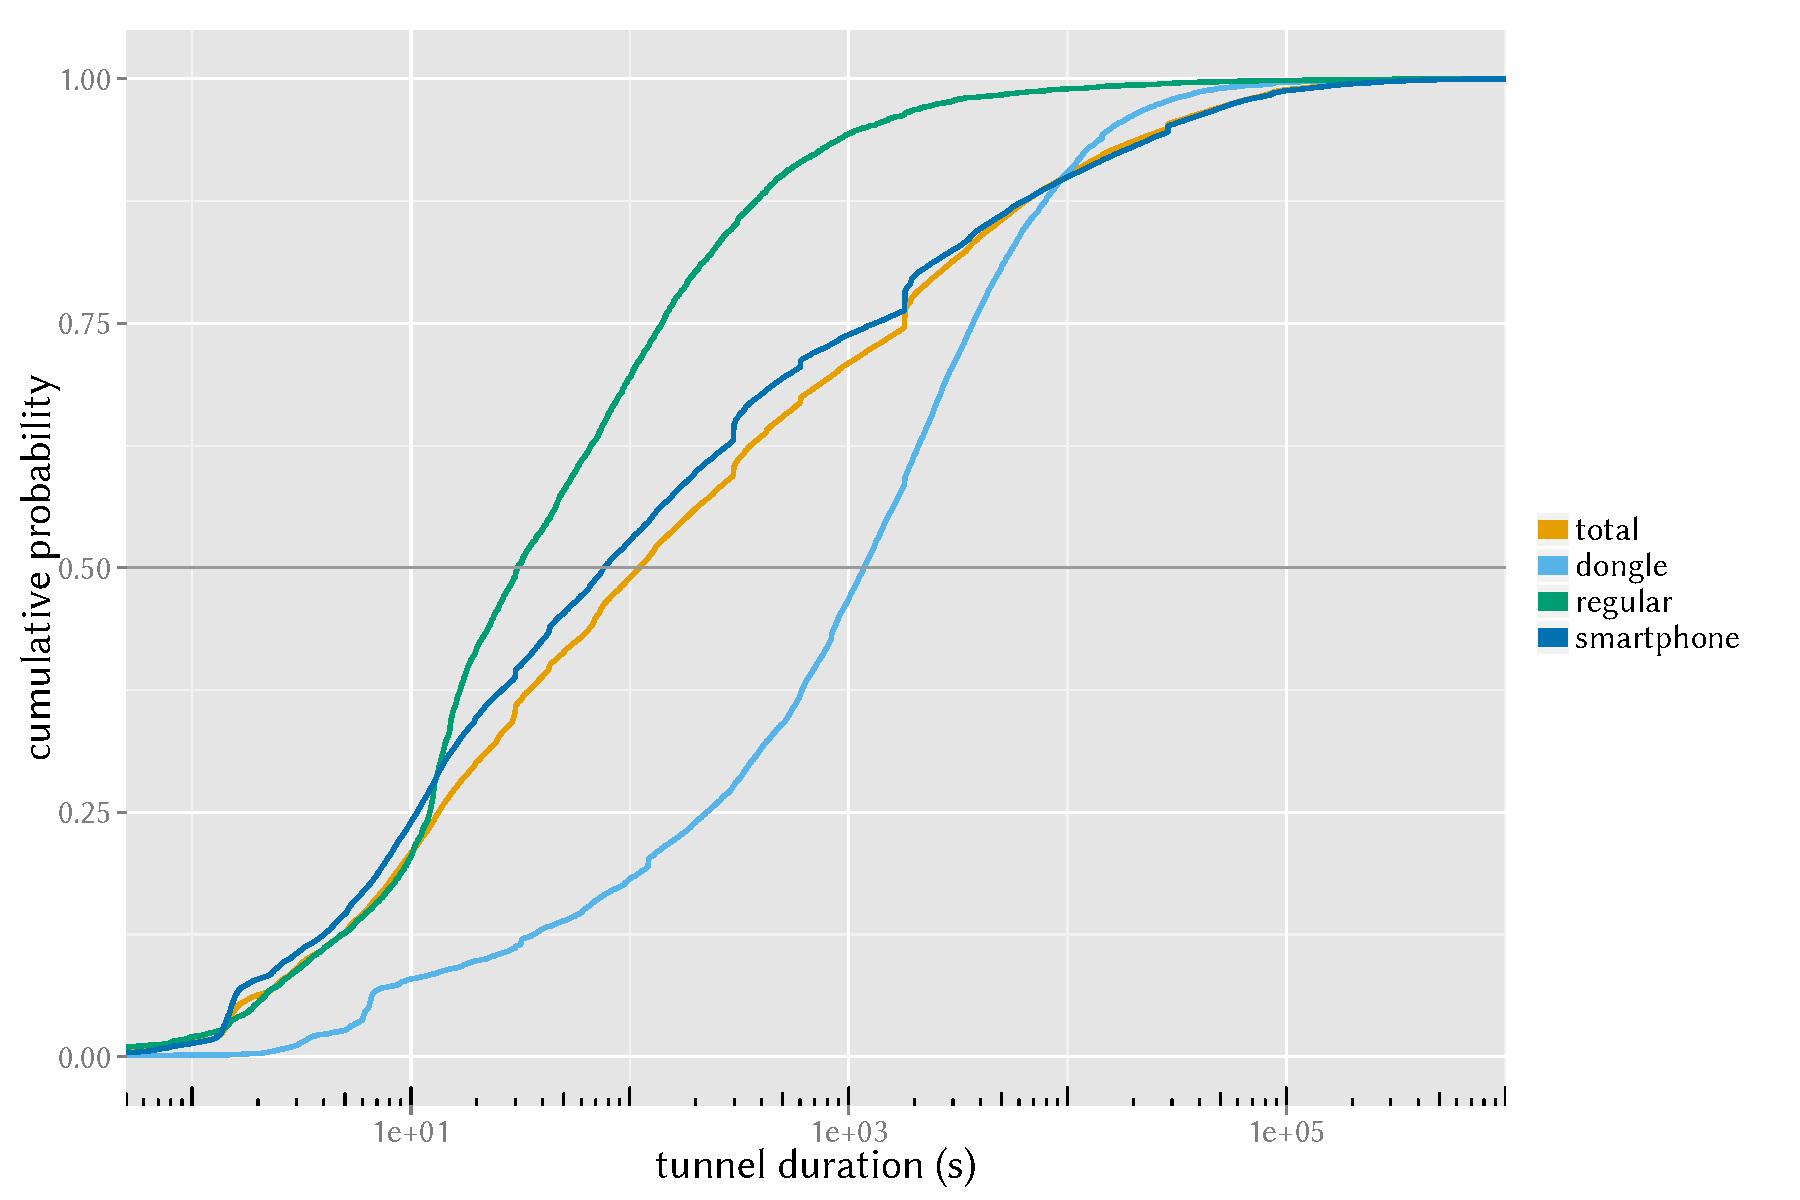
\includegraphics[width=\columnwidth]{../../chapters/041-mobilenetsmeasuring/images/R-tunnel-duration-device-type.pdf}
			\caption{Tunnel duration distribution, separated for 3G dongles, smartphones and regular phones with medians at \SI{115}{\second} (total), \SI{31}{\second} (regular), \SI{82}{\second} (smartphone), and \SI{1207}{\second} (dongle).}
		\end{figure}

		\column{0.5\textwidth}
		\begin{figure}
			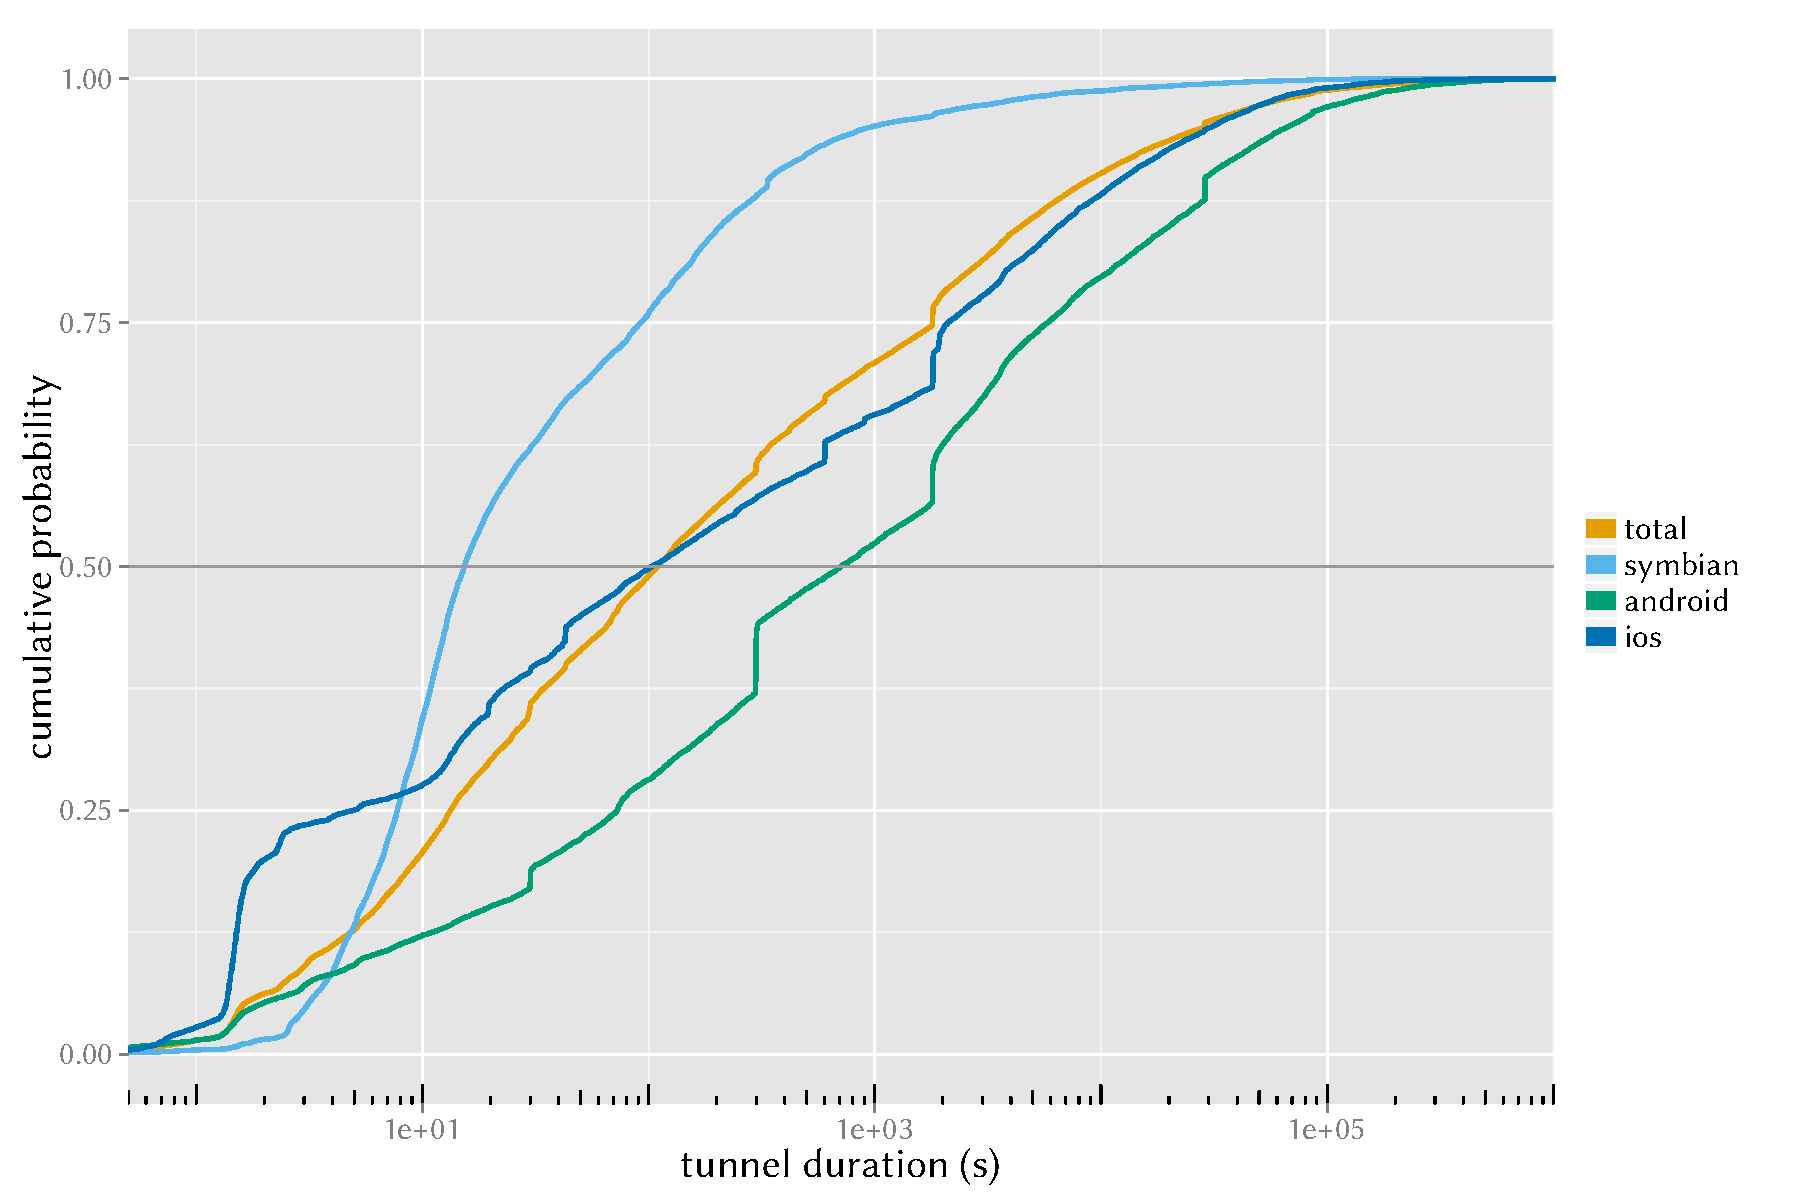
\includegraphics[width=\columnwidth]{../../chapters/041-mobilenetsmeasuring/images/R-tunnel-duration-operating-system.pdf}
			\caption{Tunnel duration CDF, separated for select OSs; Medians at \SI{115}{\second} (total), \SI{15.5}{\second} (symbian), \SI{104}{\second} (iOS), and \SI{765}{\second} (android).}
		\end{figure}
	\end{columns}
\end{frame}

\begin{frame}
	\begin{columns}[T]
		\column{0.5\textwidth}
		\begin{figure}
			\centering
			\includegraphics[width=\columnwidth]{../../chapters/041-mobilenetsmeasuring/images/R-duration-qq-category-comparison.pdf}
			\caption{Q-Q Plots of the tunnel duration distributions in comparison to device classification categories.}
		\end{figure}

		\column{0.5\textwidth}
		\begin{figure}
			\includegraphics[width=\columnwidth]{../../chapters/041-mobilenetsmeasuring/images/R-duration-classification-density.pdf}
			\caption{Logscale density plot of the tunnel duration with all classifications.}
		\end{figure}
	\end{columns}
\end{frame}

\begin{frame}
	\begin{figure}
		\centering
			\includegraphics[width=1.0\columnwidth]{../../chapters/041-mobilenetsmeasuring/images/R-create-frequency.pdf}
		\caption{Density plot of tunnel arrival rate.}
	\end{figure}
\end{frame}

\begin{frame}
	\frametitle{ECDF of the tunnel IAT in seconds by time of day}
	\begin{columns}
		\column{0.5\textwidth}
		\begin{figure}
			\includegraphics[width=0.7\columnwidth]{../../chapters/041-mobilenetsmeasuring/images/R-IAT-successful-2h-ecdfs.pdf}
			\vspace{-4mm}
			\caption{All tunnel requests.}
		\end{figure}
		\vspace{-10mm}
		\begin{figure}
			\includegraphics[width=0.7\columnwidth]{../../chapters/041-mobilenetsmeasuring/images/R-IAT-fromflows-gprs-ecdfs-2h.pdf}
			\vspace{-4mm}
			\caption{Tunnels with GPRS data flows.}
		\end{figure}

		\column{0.5\textwidth}
		\begin{figure}
			\includegraphics[width=0.7\columnwidth]{../../chapters/041-mobilenetsmeasuring/images/R-IAT-fromflows-ecdfs-2h.pdf}
			\vspace{-4mm}
			\caption{Only tunnels with data flows.}
		\end{figure}
		\vspace{-10mm}
		\begin{figure}
			\includegraphics[width=0.7\columnwidth]{../../chapters/041-mobilenetsmeasuring/images/R-IAT-fromflows-umts-ecdfs-2h.pdf}
			\vspace{-4mm}
			\caption{Tunnels with UMTS data flows.}
		\end{figure}
	\end{columns}
\end{frame}

\begin{frame}
	\begin{figure}
		\centering
		\includegraphics[height=7cm]{../../chapters/041-mobilenetsmeasuring/images/R-update-time-cdfs.pdf}
		\caption{ECDFs of the time in seconds it takes a GGSN to process a GTP update event, separately plotted for four time slots each day.}
	\end{figure}
\end{frame}

\begin{frame}
	\begin{figure}[htb]
		\centering
		\includegraphics[height=7cm]{../../chapters/041-mobilenetsmeasuring/images/R-IAT-ecdfs.pdf}
		\caption{Sampled inter-arrival time CDF and fitted theoretical distributions.}
	\end{figure}
\end{frame}

\begin{frame}
	\frametitle{Exponential Arrival Process Fits}

	\begin{center}
		\includegraphics[height=7cm]{../../chapters/041-mobilenetsmeasuring/images/R-duration-fit-cdf-facets.pdf}
	\end{center}
\end{frame}

\begin{frame}
	\frametitle{Serving Time Rational Functions Fit}

	\begin{center}
		\includegraphics[height=7cm]{../../chapters/041-mobilenetsmeasuring/images/R-IAT-active-fit-cdf-facets.pdf}
	\end{center}
\end{frame}


\begin{frame}
	\begin{table}
	\tiny
	\caption{Parameters for the exponentially distributed inter-arrival times and corresponding Pearson correlation coefficients.}
		\centering
		\begin{tabu}{X[0.9,l]X[r]X[r]} 
		\toprule
		\textbf{Time of Day} & $\mathbf{\lambda}$ & $\mathbf{R_{arrival}}$\\ 
		\midrule
		0h-5h   & $10.67477$ & $0.995$ \\
		6h-11h  & $24.53298$ & $0.992$ \\
		12h-17h & $29.2504$  & $0.993$ \\
		18h-23h & $23.49983$ & $0.986$ \\
		\bottomrule
		\end{tabu}
	\end{table}

	\begin{table}
	\tiny
	\caption{Inverse rational functions fitted to the ECDFs of the tunnel duration by time of day and correlation coefficients of the fit.}
		\centering
		\begin{tabu}{X[1.1,l]X[4.5,r]X[r]} 
		\toprule
		\textbf{Time of Day} & \textbf{Inverse Serving Time CDF Representation} & $\mathbf{R_{dur}}$\\ 
		\midrule
		0h-5h & $0.919208 - 60.6136y - 3498.78y^3 - \frac{110.707y + 2289.94y^3}{y - 1.00469}$ &  $0.999$ \\
		6h-11h & $1 + 117.484y - 368.643y^2 - \frac{1720.13y^4}{y - 1.0041}$ & $0.999$ \\
		12h-17h & $0.952566 + 69.4907y + \frac{81146.1y^3 + 1.08572\times10^6y^5}{805 - 802.01y}$ & $0.999$ \\
		18h-23h & $0.911924 + 82.0562y - \frac{2936.93y^4}{1.94468y - 1.9532}$ & $0.999$ \\
		\bottomrule
		\end{tabu}
	\end{table}
\end{frame}


\begin{frame}
	\frametitle{Queuing Models}
	\begin{center}
		\includegraphics[height=2cm]{../../chapters/041-mobilenetsmeasuring/images/GGn-model.pdf}
	\end{center}

	Described by Kendall's Notation $A/S/c/q$
	\begin{itemize}
	\item Distribution of the arrival process $A$
		% \begin{itemize}
		% 	\item Poisson arrivals, memoryless
		% 	\item Markov chain model
		% \end{itemize}
	\item Distribution of the serving time $S$
	\item Number of Servers $c$
	\item Queue Length $q$
	\begin{itemize}
		\item $q=\infty$ no loss will occur
		\item $0$ loss/blocking system, no queue
	\end{itemize}
	\item Evaluate
		\begin{itemize}
			\item Average queue length and server occupation
			\item Blocking probability
		\end{itemize}
	\end{itemize}
\end{frame}

\begin{frame}
	\begin{figure}
		\includegraphics[height=1cm]{../../chapters/041-mobilenetsmeasuring/images/markovchain.pdf}
		\caption{$M/M/c/\infty$ Markov chain model.}
	\end{figure}
\end{frame}

\begin{frame}
	\begin{columns}
		\column{0.5\textwidth}
		\begin{figure}
			\includegraphics[width=\columnwidth]{../../chapters/041-mobilenetsmeasuring/images/R-monolithic-blocking.pdf}
			\caption{Impact of the number of supported parallel tunnels on the blocking probability for the traditional GGSN model.}
		\end{figure}

		\column{0.5\textwidth}
		\begin{figure}
			\includegraphics[width=\columnwidth]{../../chapters/041-mobilenetsmeasuring/images/R-monolithic-tunnelusage.pdf}
			\caption{Mean number of tunnels concurrently served by the GGSN for incrementally increasing capacity.}
		\end{figure}
	\end{columns}
\end{frame}

\begin{frame}
	\begin{figure}
		\includegraphics[height=7cm]{../../chapters/041-mobilenetsmeasuring/images/R-virtualized-tunnelusage.pdf}
		\caption{Comparison of the mean tunnel capacity usage of the individual virtual instance configurations.}
	\end{figure}
\end{frame}

\begin{frame}
	\begin{figure}
		\includegraphics[height=7cm]{../../chapters/041-mobilenetsmeasuring/images/R-virtualized-mean-instanceusage.pdf}
		\caption{Mean instance usage of various virtualization configurations. A higher number of total instances results in a finer granularity of scaling and energy efficiency as more instances can be kept shut down.}
	\end{figure}
\end{frame}

\begin{frame}
	\frametitle{}
	\begin{figure}
		\includegraphics[height=7cm]{../../chapters/041-mobilenetsmeasuring/images/compare-maxinstances-block.pdf}
		\caption{Influence of start up and shut down time on blocking probability with regard to different numbers of instances.}
	\end{figure}
\end{frame}

\begin{frame}
	\begin{figure}
		\includegraphics[height=7cm]{../../chapters/041-mobilenetsmeasuring/images/R-virtualized-startstop-blocking-barchart.pdf}
		\caption{Influence of the boot and shutdown time on the blocking probability.}
	\end{figure}
\end{frame}

\begin{frame}
	\frametitle{Scaling Up or Out with a Virtualized GGSN}
	
	\begin{center}
		\includegraphics[height=7cm]{../../chapters/041-mobilenetsmeasuring/images/R-virtualized-instanceuse-barplot.pdf}
	\end{center}
\end{frame}

\begin{frame}
	\begin{figure}
		\centering
		\includegraphics[height=6cm]{../../chapters/041-mobilenetsmeasuring/images/R-virtualized-startstop-tunnelusage-blocking-comparison.pdf}
		\caption{Trade-off between blocking probability and mean resource utilization with regard to maximum number of instances, instance tunnel capacity, and start and stop time.}
	\end{figure}
\end{frame}

\begin{frame}
	\begin{table}
	\caption{Effect sizes of the simulation parameters based on a one-way ANOVA.}
		\scriptsize
		\centering
		\begin{tabu}{X[2.5,l]X[1.0,r]X[0.6,r]X[0.6,r]X[0.6r]}
		\toprule
		& $\mathbf{F-ratio}$ & $\mathbf{p-value}$ & $\mathbf{\eta^2}$ & $\mathbf{{\omega}^2}$\\ 
		\midrule
		\multicolumn{2}{c}{\textbf{Blocking probability}} & & & \\ 
		Individual instance tunnel capacity & $104$ & $<0.001$ & $0.468$ & $0.463$\\ %F(12, 1417)=
		Number of instances & $9.29$ & $<0.001$ & $0.056$ & $0.050$\\ %F(9,1420)=
		Start/stop duration & $0.21$ & $0.931$ & $<0.001$ & $0.002$\\ %F(4,1425)=
		Total tunnel capacity & $317257$ & $<0.001$ & $0.999$ & $0.999$ \\ %F(12,1417=
		\midrule
		\multicolumn{2}{c}{\textbf{Mean number of tunnels}}& & & \\ 
		Individual instance tunnel capacity & $105.7$ & $<0.001$ & $0.472$ & $0.467$\\ %F(12,1417)=
		Number of instances & $9.39$ & $<0.001$ & $0.056$ & $0.050$\\ %F(9,1420)=
		Start/stop duration & $0.25$ & $0.912$ & $<0.001$ & $0.002$\\ %F(4,1425)=
		Total tunnel capacity & $365753$ & $<0.001$ & $0.999$ & $0.999$ \\ %F(12,1417)=
		\bottomrule
		\end{tabu}
	\end{table}
\end{frame}





\begin{frame}
	\begin{figure}
		\includegraphics[height=5cm]{../../chapters/05-mobilestreaming/images/layer-timescales.pdf}
		\caption{Approximate discernible time scales the networking stack protocols operate on in each layer.}
	\end{figure}
\end{frame}

\begin{frame}
	\frametitle{TCP Changes in the Linux Kernel}
		\tiny
		\begin{tabu}{X[1.4]X[0.4]X[0.4]X[0.7]}
		\toprule
		\textbf{Change} & \textbf{Related Work} & \textbf{Kernel} & \textbf{Date} \\
		\midrule
		BIC as default congestion avoidance algorithm (from Reno) & & 2.6.8 & August 2004 \\
		CUBIC as default congestion avoidance algorithm & \cite{ha2008cubic} & 2.6.19 & November 2006 \\
		New TCP Slow Start: HyStart & \cite{Ha20112092} & 2.6.29 & March 2009 \\
		Multipath TCP & \cite{rfc6824} & external & 2011 \\
		TCP User Timeout & \cite{rfc5482} & 2.6.37 & January 2011 \\
		Initial Receive Window \SI{10}{MSS} & \cite{rfc6928} & 2.6.38 & March 2011 \\
		Initial Congestion Window \SI{10}{MSS} & \cite{rfc6928} & 2.6.39 & May 2011 \\
		\SI{1}{\second} initial RTO (from \SI{3}{\second}) & \cite{rfc6298} & 3.1 & October 2011 \\
		Changes to sstresh and CWND bevahior & \cite{rfc5681} & 3.1 & October 2011 \\ % details: https://git.kernel.org/cgit/linux/kernel/git/torvalds/linux.git/commit/?id=9ad7c049f0f79c418e293b1b68cf10d68f54fcdb
		TCP Proportional Rate Reduction & \cite{rfc6937} & 3.2 & January 2012 \\
		Byte queue limits and TCP buffer limits &  & 3.3 & March 2012 \\ % https://lwn.net/Articles/454390/
		CoDel AQM & \cite{nichols2014codel} & 3.5 & July 2012 \\
		TCP Early Retransmit & \cite{rfc5827} & 3.5 & July 2012 \\
		TCP small queues & & 3.6 & September 2012 \\ %http://lwn.net/Articles/507065/
		TCP Fast Open (client side) & \cite{cheng2014tcptfo} & 3.6 & September 2012 \\
		TCP Fast Open (server side) & & 3.7 & December 2012 \\
		TCP tail loss probe & & 3.10 & June 2013 \\ % http://tools.ietf.org/html/draft-dukkipati-tcpm-tcp-loss-probe-01
		TCP Forward RTO-Recovery & \cite{rfc5682} & 3.10 & June 2013 \\
		Low latency network polling & & 3.11 & September 2013 \\ %http://lwn.net/Articles/551284/ and http://www.linuxplumbersconf.org/2012/wp-content/uploads/2012/09/2012-lpc-Low-Latency-Sockets-slides-brandeburg.pdf
		Improved RTO calculation and handling of reordering & & 3.12 & November 2013 \\ % https://git.kernel.org/cgit/linux/kernel/git/torvalds/linux.git/commit/?id=0f7cc9a3c2bd89b15720dbf358e9b9e62af27126 and https://git.kernel.org/cgit/linux/kernel/git/torvalds/linux.git/commit/?id=ed08495c31bb991de636d2488abaa50b39f2ff4a
		TCP Fast Open enabled by default & & 3.13 & January 2014 \\
		TCP auto corking & & 3.14 & March 2014 \\ % https://git.kernel.org/cgit/linux/kernel/git/torvalds/linux.git/commit/?id=f54b311142a92ea2e42598e347b84e1655caf8e3
		PIE AQM & & 3.14 & March 2014 \\ % http://tools.ietf.org/html/draft-pan-aqm-pie-01 and https://git.kernel.org/cgit/linux/kernel/git/torvalds/linux.git/commit/?id=d4b36210c2e6ecef0ce52fb6c18c51144f5c2d88
		TCP Fast Open over IPv6 & & 3.16 & 2014 \\
		LISP & \cite{rfc6830} & 3.16 & 2014 \\
		\bottomrule
		\end{tabu}
\end{frame}





\begin{frame}
	\frametitle{Sensorium}
	\begin{columns}
		\column{0.5\textwidth}
		\begin{figure}
			\includegraphics[width=0.6\columnwidth]{../../chapters/06-mobilestreamingmeasurements/images/sensorium.png}
		\end{figure}

		\column{0.5\textwidth}
		\begin{figure}
			\includegraphics[width=0.6\columnwidth]{../../chapters/06-mobilestreamingmeasurements/images/sensorium-settings.png}
		\end{figure}
	\end{columns}
\end{frame}

\begin{frame}
	\begin{figure}
		\includegraphics[height=6cm]{../../chapters/06-mobilestreamingmeasurements/images/o3gm.png}
		\caption{The O3GM web page, displaying a 3G coverage measurements layer with data collected by Sensorium on top of the OpenStreetMap base layer.}
	\end{figure}
\end{frame}



\begin{frame}
	\begin{figure}
		\centering
		\includegraphics[height=2cm]{../../chapters/06-mobilestreamingmeasurements/images/streaming-hybrid.pdf}
		\caption{Future testbed iteration: hybrid of ns-3 LTE simulation and actual or emulated streaming client and server bridged to it.}
	\end{figure}
\end{frame}

\begin{frame}
	\begin{columns}
		\column{0.5\textwidth}
		\begin{figure}
			\includegraphics[width=\columnwidth]{../../chapters/06-mobilestreamingmeasurements/images/R-ltesim-bwseries-stallduration.pdf}
			\caption{Relative stalling duration of the simulated reliable streaming player under limited Internet bandwidth.}
		\end{figure}

		\column{0.5\textwidth}
		\begin{figure}
			\includegraphics[width=\columnwidth]{../../chapters/06-mobilestreamingmeasurements/images/R-ltesim-bwseries-numstalls.pdf}
			\caption{Number of stalling events of the simulated reliable streaming player under limited Internet bandwidth.}
		\end{figure}
	\end{columns}
\end{frame}

\begin{frame}
	\begin{columns}
		\column{0.5\textwidth}
		\begin{figure}
			\includegraphics[width=\columnwidth]{../../chapters/06-mobilestreamingmeasurements/images/R-ltesim-latencyseries-stallduration.pdf}
			\caption{Relative stalling duration of the simulated reliable streaming player under increased Internet latency.}
		\end{figure}

		\column{0.5\textwidth}
		\begin{figure}
			\includegraphics[width=\columnwidth]{../../chapters/06-mobilestreamingmeasurements/images/R-ltesim-latencyseries-numstalls.pdf}
			\caption{Number of stalling events of the simulated reliable streaming player under increased Internet latency.}
		\end{figure}
	\end{columns}
\end{frame}


\setcounter{framenumber}{\value{finalframe}}

\end{document}


